\documentclass[11pt,a4paper]{ipmu}

% Packages
\usepackage{natbib}     % For bibliography
\usepackage{caption}    % Better control of figure captions
\usepackage{subcaption} % Subfigures
\usepackage{aas_macros}
\usepackage{rotating}   % For rotating figures
\usepackage{booktabs}
\usepackage{enumitem}
\usepackage{comment}

% Set Thesis Metadata
\setThesisTitle{Effects of Replicated N-body Simulation Boxes \\in Simulating Weak Lensing Observables}
\setThesisJapaneseTitle{弱重力レンズ統計量の模擬データ生成における\\有限体積のN体シミュレーションの影響の研究}
\setThesisAuthorEnglish{Akira Tokiwa}
\setThesisAuthorJapanese{常盤 晟}

\begin{document}

% Create Title Page
\makethesistitle

% Create Abstract Page
% \begin{abstractpage}
%     We investigate the influence of super-sample covariance on the covariance and correlation matrices of the power spectrum and higher-order statistics using two distinct simulation approaches: BIGBOX and TILED. Leveraging 11 realizations of state-of-the-art BIGBOX simulations from the HalfDome project, each containing $6144^3$ particles within a 3750 Mpc/h volume, and 20 TILED realizations composed of smaller $1024^3$-particle boxes within 625 Mpc/h, we analyze the convergence field under the Born approximation. Uniformly covering the full sky with $10^\circ \times 10^\circ$ patches extracted via a Fibonacci grid, we employ a comprehensive suite of higher-order statistics, including bispectrum, probability distribution function, peak and minima counts, and Minkowski functionals, and the angular power spectrum to probe the non-Gaussian features of the convergence maps.

Our comparative analysis reveals that mean statistical measures between BIGBOX and TILED simulations agree within 1\% across all statistics, redshifts, and multipoles, validating the simulations' reliability in capturing the underlying cosmological model. However, variance ratios exhibit significant differences of 10-30\%, particularly at high multipoles and redshifts, attributable to super-sample covariance arising from large-scale modes present in BIGBOX but absent in TILED. Shape noise impacts statistical measures, especially the angular power spectrum and peak/minima counts, yet super-sample covariance remains the dominant effect. Additionally, Gaussian smoothing affects small-scale features without substantially variating the covariance and correlation structures, while box replication artifacts introduce systematic biases by underestimating mean angular power spectra and distorting higher-order statistics.

These findings underscore the critical role of super-sample covariance in high-precision cosmological analyses, particularly for upcoming weak lensing surveys such as LSST, Euclid, and Roman. Accurate variance modeling necessitates the inclusion of large-scale modes in simulations, while maintaining robustness against shape noise and smoothing operations. Addressing systematic challenges like box replication artifacts is essential to prevent biases in the interpretation of higher-order statistics. Future work will focus on mitigating replication artifacts, incorporating diverse cosmological models and baryonic effects, and integrating these insights into survey design and data analysis pipelines to enhance the precision of cosmological parameter inference. Our study advances simulation techniques and observational strategies, reinforcing weak lensing as a pivotal tool for probing the Universe's fundamental properties with unprecedented accuracy.
% \end{abstractpage}

\tableofcontents  % Generates the table of contents
\listoffigures    % Optional: List of figures
\listoftables     % Optional: List of tables

% \chapter{Introduction}
% \input{introduction}

%chapter{Cosmology (Finished)}
%\input{background/cosmology}

%\chapter{CMB Power Spectrum (Omit)}
%\input{background/history}

\chapter{Weak Lensing}
Weak gravitational lensing (WL), also known as cosmic shear, refers to the subtle distortions in the images of distant source caused by the gravitational fields of intervening mass distributions. Unlike strong lensing, which produces noticeable effects such as multiple images or arcs, weak lensing induces small, coherent distortions that require statistical analysis to detect and interpret. For the standard approach to lensing, we refer to \citet{1992grle.book.....S}, \citet{2001PhR...340..291B} and \citet{2010CQGra..27w3001B}.

\section{Lens Equation}
\subsection{Derivation}
To derive the lens equation, we consider a perturbed FLRW metric, which incorporates gravitational potential perturbations. The metric is expressed as
\begin{equation}
    ds^2 = -\left(1 + \frac{2\Phi}{c^2}\right)c^2 dt^2 + a^2(t) \left(1 - \frac{2\Psi}{c^2}\right) \left[ d\chi^2 + f_K^2(\chi) \, \omega_{ab} \, dx^a dx^b \right] \quad (a, b = 2, 3),
    \label{eq:perturbed_metric}
\end{equation}
where the angular part of the metric is defined by
\begin{equation}
    \omega_{ab} \, dx^a dx^b := d\theta^2 + \sin^2 \theta \, d\phi^2.
    \label{eq:angular_metric}
\end{equation}
In this context, \( \Phi \) and \( \Psi \) represent the scalar gravitational potentials, and \( f_K(\chi) \) encodes the spatial curvature as previously defined in Eq.~\eqref{eq:fk_definition}.

The trajectory of light within this spacetime is governed by the geodesic equation, which is given by
\begin{equation}
    \frac{d^2 x^\mu}{d\lambda^2} + \Gamma^\mu_{\alpha \beta} \frac{dx^\alpha}{d\lambda} \frac{dx^\beta}{d\lambda} = 0,
    \label{eq:geodesic_equation}
\end{equation}
where \( \lambda \) is an affine parameter and \( \Gamma^\mu_{\alpha \beta} \) are the Christoffel symbols corresponding to the metric in Equation~\eqref{eq:perturbed_metric}.
To facilitate the derivation, we reparametrize the geodesic equation by substituting the affine parameter \( \lambda \) with the comoving radial distance \( \chi \). Applying the chain rule, the geodesic equation transforms to
\begin{equation}
    \frac{d^2 x^\mu}{d\chi^2} + \Gamma^\mu_{\alpha \beta} \frac{dx^\alpha}{d\chi} \frac{dx^\beta}{d\chi} - \frac{d^2 \lambda}{d\chi^2} \left( \frac{d\lambda}{d\chi} \right)^{-1} \frac{dx^\mu}{d\chi} = 0.
    \label{eq:geodesic_reparametrized}
\end{equation}
Setting \( \mu = 1 \) (where \( x^1 = \chi \)) in Equation~\eqref{eq:geodesic_reparametrized} and simplifying, we obtain
\begin{equation}
    \frac{d^2 x^\mu}{d\chi^2} + \left( \Gamma^\mu_{\alpha \beta} - \Gamma^1_{\alpha \beta} \right) \frac{dx^\alpha}{d\chi} \frac{dx^\beta}{d\chi} = 0.
    \label{eq:geodesic_mu1}
\end{equation}
The evaluation of Equation~\eqref{eq:geodesic_mu1} requires the computation of the Christoffel symbols. Additionally, the derivative \( c \, dt / d\chi \) is derived from the null condition
\begin{equation}
    g_{\mu \nu} \frac{dx^\mu}{d\chi} \frac{dx^\nu}{d\chi} = 0,
    \label{eq:null_condition}
\end{equation}
yielding
\begin{equation}
    \frac{c \, dt}{d\chi} = -a(t) \left[ 1 - \frac{\Phi}{c^2} - \frac{\Psi}{c^2} + \frac{f_K^2(\chi)}{2} \omega_{ab} \frac{dx^a}{d\chi} \frac{dx^b}{d\chi} \right],
    \label{eq:dt_dchi}
\end{equation}
valid to first order in \( \Phi \) and second order in \( dx^a / d\chi \). Notably, for the evaluation of Equation~\eqref{eq:geodesic_mu1}, only the zeroth-order term \( c \, dt / d\chi = -a(t) \) is required. However, the inclusion of perturbative terms in Equation~\eqref{eq:dt_dchi} is essential for subsequent derivations of the lens equation.

Focusing on the angular components (\( \mu = a \)) of Equation~\eqref{eq:geodesic_mu1}, we derive the following differential equation:
\begin{equation}
    \frac{d^2 x^a}{d\chi^2} + 2 \frac{f_K'(\chi)}{f_K(\chi)} \frac{dx^a}{d\chi} + \omega^{ab} \frac{\Phi_b + \Psi_b}{c^2 f_K^2(\chi)} = 0,
    \label{eq:geodesic_angular}
\end{equation}
where \( \Phi_b \) and \( \Psi_b \) denote the derivatives of the gravitational potentials with respect to the angular coordinates \( x^a \).
Integrating Equation~\eqref{eq:geodesic_angular} twice with respect to \( \chi \), we obtain
\begin{eqnarray}
    x^a(\chi_s) - x^a(0) &=& -\frac{1}{c^2} \int_0^{\chi_s} d\chi' \int_0^{\chi'} d\chi \, \omega_{ab} \left[ \Phi_b(\chi, \theta(\chi)) + \Psi_b(\chi, \theta(\chi)) \right] \nonumber \\
    &=& -\frac{1}{c^2} \int_0^{\chi_s} d\chi \, \omega_{ab} \left[ \Phi_b(\chi, \theta(\chi)) + \Psi_b(\chi, \theta(\chi)) \right] \int_{\chi}^{\chi_s} d\chi' \frac{1}{f_K^2(\chi')} \nonumber \\
    &=& -\frac{1}{c^2} \int_0^{\chi_s} d\chi \, \omega_{ab} \left[ \Phi_b(\chi, \theta(\chi)) + \Psi_b(\chi, \theta(\chi)) \right] \frac{f_K(\chi_s - \chi)}{f_K(\chi_s)f_K(\chi)},
    \label{eq:xa_integrated}
\end{eqnarray}
where \( \chi_s \) denotes the comoving radial distance to the source, and \( x^a(0) \) is the angular position at the observer's location.
Defining $(\nabla_\theta)^a = \omega^{ab} \partial_b$, the angular position of the source galaxy $\boldsymbol{\beta}$ is related to the observed angular position $\boldsymbol{\theta}$ by
\begin{equation}
    \boldsymbol{\theta}(\chi_s) = \boldsymbol{\theta}(0) - \frac{1}{c^2} \int_0^{\chi_s} d\chi \, \nabla_\theta \left[ \Phi\left(\chi, \boldsymbol{\theta}(\chi)\right) + \Psi\left(\chi, \boldsymbol{\theta}(\chi)\right) \right] \frac{f_K(\chi_s - \chi)}{f_K(\chi_s)f_K(\chi)}.
    \label{eq:lens_equation}
\end{equation}
Applying the Born approximation \citep{1926ZPhy...38..803B}, and assume that $\Phi = \Psi$, we can simplify the lens equation to:
\begin{equation}
    \boldsymbol{\theta}(\chi_s) = \boldsymbol{\theta}(0) - \frac{2}{c^2} \int_0^{\chi_s} d\chi \, \nabla_\theta \left[ \Phi\left(\chi, \boldsymbol{\theta}(0)\right) \right]\frac{f_K(\chi_s - \chi)}{f_K(\chi_s)f_K(\chi)}.
    \label{eq:lens_equation_born}
\end{equation}
This final expression constitutes the lens equation, encapsulating the deflection of light due to the gravitational potentials \( \Phi \) and \( \Psi \) along the line of sight. 

\subsection{Lensing Matrix}
\begin{figure}[ht]
    \centering
    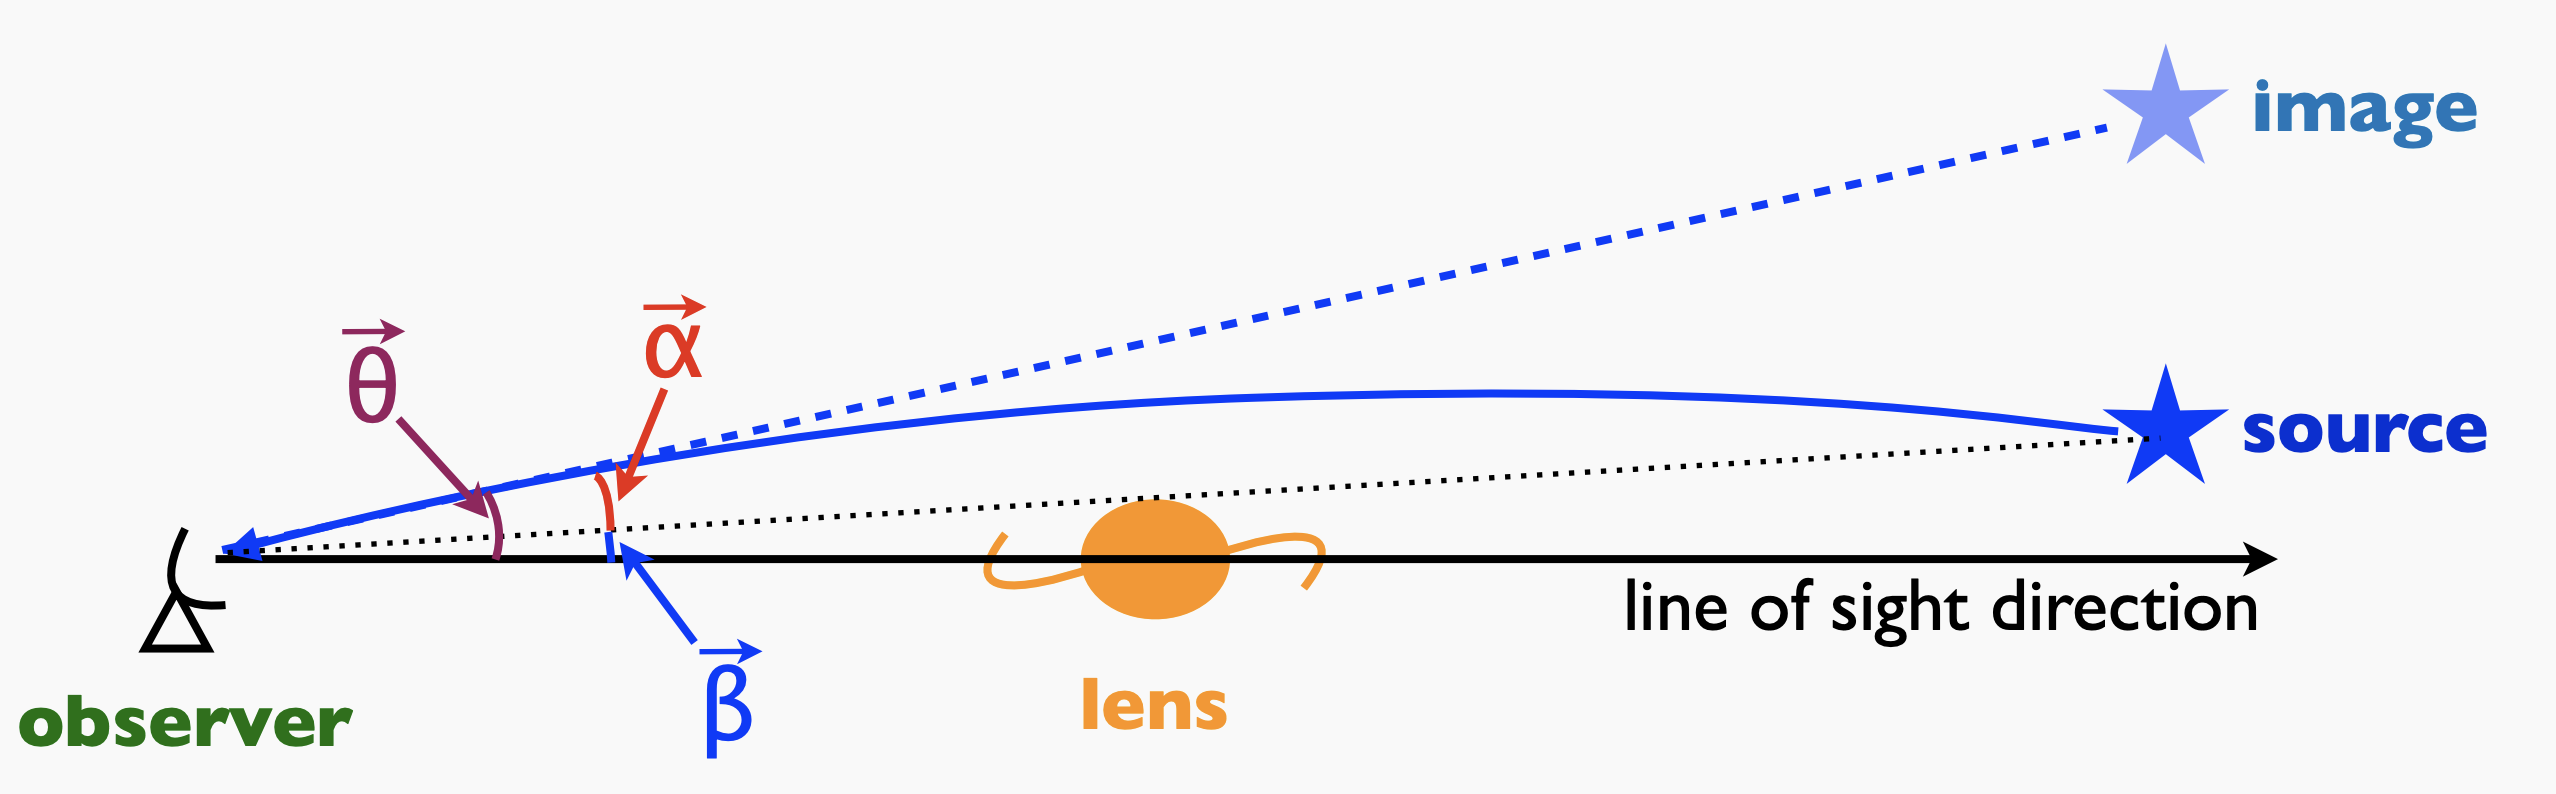
\includegraphics[width=\textwidth]{figures/Lens_overview_Oguri.png}
    \caption{Schematic representation of the lensing geometry. The source is located at $\boldsymbol{\beta}$, while the observed image is at $\boldsymbol{\theta}$. The deflection angle $\boldsymbol{\alpha}$ is the difference between the observed and true angular positions.}
    \label{fig:lens_geometry}
\end{figure}
Redefining the notation in Eq.~\eqref{eq:lens_equation_born} and considering the angular position of the source $\boldsymbol{\beta} = \boldsymbol{\theta}(\chi_s)$ and the observed angular position $\boldsymbol{\theta} = \boldsymbol{\theta}(0)$ (see Fig.~\ref{fig:lens_geometry}), we can express the lens equation as \citep{2001PhR...340..291B, 2009A&A...499...31H, 2015RPPh...78h6901K}:
\begin{equation}
    \boldsymbol{\beta} = \boldsymbol{\theta} - \boldsymbol{\alpha}(\boldsymbol{\theta}),
    \label{eq:lens_equation_vector}
\end{equation}
where the deflection angle \( \boldsymbol{\alpha}(\boldsymbol{\theta}) \) is defined by:
\begin{equation}
    \boldsymbol{\alpha}(\boldsymbol{\theta}) = \nabla_{\boldsymbol{\theta}} \psi(\boldsymbol{\theta}), \quad \psi(\boldsymbol{\theta}) = \frac{2}{c^2} \int_0^{\chi_s} d\chi \, \frac{f_K(\chi_s - \chi)}{f_K(\chi_s)f_K(\chi)} \Phi\left(f_K(\chi) \boldsymbol{\theta}, \chi\right).
    \label{eq:deflection_angle}
\end{equation}
The mapping between the source plane and the image plane can be described by the Jacobian matrix $\mathcal{A}$, which relates infinitesimal displacements in the source position to displacements in the image position:
\begin{equation}
\label{eq:jacobian_matrix}
    \mathcal{A} := \frac{\partial \boldsymbol{\beta}}{\partial \boldsymbol{\theta}} = 
    \begin{pmatrix}
        1 - \kappa - \gamma_1 & -\gamma_2 \\
        -\gamma_2 & 1 - \kappa + \gamma_1
    \end{pmatrix}
    = \left(1 - \kappa \right) 
    \begin{pmatrix}
        1 & 0 \\
        0 & 1
    \end{pmatrix}
    - |\gamma|
    \begin{pmatrix}
        \cos{2\phi} & \sin{2\phi} \\
        \sin{2\phi} & -\cos{2\phi}
    \end{pmatrix},
\end{equation}
where $\kappa$ is the convergence and $\gamma = \gamma_1 + i\gamma_2 = |\gamma| e^{2i\phi}$ is the shear.
The quantities $\kappa$ and $\gamma$ will be discussed in detail in the subsequent sections.
Figure~\ref{fig:distortion} illustrates the effects of gravitational lensing on the shapes of background sources through the lensing matrix $\mathcal{A}$. The panels demonstrate how the combined effects of convergence and shear components in the Jacobian matrix $\mathcal{A}$ lead to complex distortions of background sources.
\begin{figure}[ht]
    \centering
    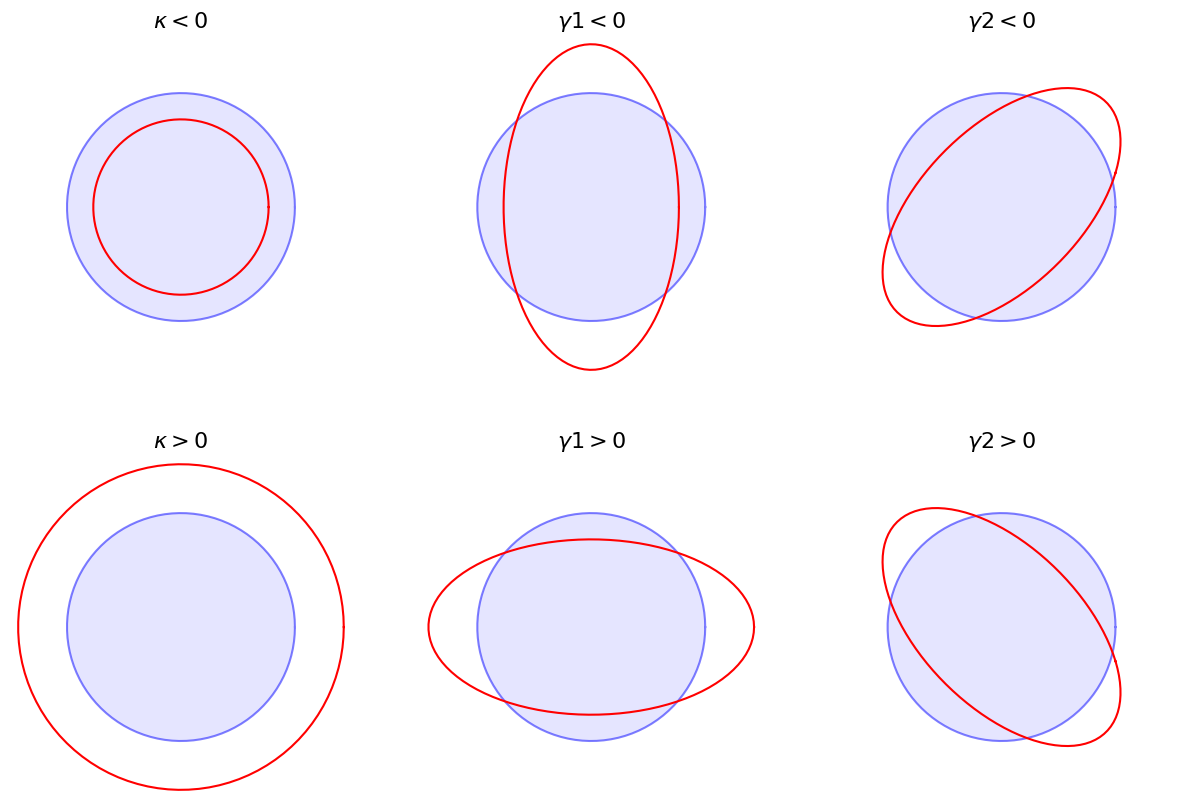
\includegraphics[width=0.8\textwidth]{figures/distortion.png}
    \caption{Illustration of the distortion of background sources due to gravitational lensing. The left panel depict the effect of the convergence $\kappa$ and the middle and right panels show the components of the shear $\gamma = \gamma_1 + i\gamma_2$ on circular background sources. Positive and negative values of $\kappa$ cause isotropic magnification or demagnification, while $\gamma_1$ and $\gamma_2$ introduce anisotropic distortions, stretching the sources along or at an angle to the principal axes.}
    \label{fig:distortion}
\end{figure}

\section{Convergence}
\subsection{Definition}
From the lensing matrix in Eq.~\eqref{eq:jacobian_matrix}, the convergence $\kappa$ is defined as:
\begin{equation}
    \label{eq:convergence}
        \kappa(\boldsymbol{\theta}) := \frac{1}{2} \left( \frac{\partial^2 \psi}{\partial \theta_1^2} + \frac{\partial^2 \psi}{\partial \theta_2^2} \right) = \frac{1}{2} \nabla_{\boldsymbol{\theta}}^2 \psi(\boldsymbol{\theta})
\end{equation}
with $\theta_1$ and $\theta_2$ representing the angular coordinates on the sky.
In Fourier space, the convergence field could be expressed as:
\begin{equation}
    \label{eq:fourier_convergence}
    \tilde{\kappa}(\boldsymbol{\ell}) = \int d^2\theta \, e^{-i\boldsymbol{\ell} \cdot \boldsymbol{\theta}} \kappa(\boldsymbol{\theta}) = \frac{1}{2} \ell^2 \tilde{\psi}(\boldsymbol{\ell}),
\end{equation}
where $\tilde{(\quad)}$ denotes the Fourier transform of the corresponding quantity and $\ell = |\boldsymbol{\ell}|$ is the Fourier counterpart to the angular position $\boldsymbol{\theta}$.
\subsection{Convergence from Density Contrast}
In a flat universe, the Poisson equation in comoving coordinates is expressed as
\begin{align}
\label{eq:poisson_flat}
    \nabla_{\mathbf{x}}^2 \Phi(\mathbf{x}, \chi) &= 4\pi G a^2(\chi) \bar{\rho}_m(\chi) \delta(\mathbf{x}, \chi) \nonumber\\ 
    &= 4\pi G a^2(\chi) \left[ \frac{3 H_0^2 \Omega_m}{8 \pi G} a^{-3}(\chi) \right] \delta(\mathbf{x}, \chi) \nonumber \\ 
    &= \frac{3}{2} \Omega_m H_0^2 a^{-1}(\chi) \delta(\mathbf{x}, \chi),
\end{align}
where we utilized Eq.~\eqref{eq:friedmann_rewritten} and Eq.~\eqref{eq:critical_density}.
Substituting the expression for $\Phi$ from Eq.~\eqref{eq:poisson_flat} into the lensing potential (Eq.~\eqref{eq:deflection_angle}) and subsequently into the convergence (Eq.~\eqref{eq:convergence}), we derive:
\begin{eqnarray}
    \label{eq:convergence_integral}
    \kappa(\boldsymbol{\theta}) 
    &=& \frac{1}{2} \nabla_{\boldsymbol{\theta}}^2 \psi(\boldsymbol{\theta}) \nonumber \\
    &=& \frac{1}{c^2} \int_0^{\chi_s} \mathrm{d}\chi \, \frac{f_K(\chi_s - \chi)}{f_K(\chi_s) f_K(\chi)} \nabla_{\boldsymbol{\theta}}^2 \Phi\left(f_K(\chi) \boldsymbol{\theta}, \chi\right) \nonumber \\
    &=& \frac{1}{c^2} \int_0^{\chi_s} \mathrm{d}\chi \, \frac{f_K(\chi_s - \chi)}{f_K(\chi_s) f_K(\chi)} \left[ \frac{1}{f_K^2(\chi)} \nabla_{\mathbf{x}}^2 \Phi\left(\mathbf{x}, \chi\right) \right] \nonumber \\
    &=& \int_0^{\chi_s} \mathrm{d}\chi \, \frac{3 \Omega_m H_0^2}{2 c^2} \, \frac{f_K(\chi_s - \chi) f_K(\chi)}{f_K(\chi_s)} \frac{a^{-1}(\chi)}{f_K^3(\chi)} \delta\left(\mathbf{x}, \chi\right) \nonumber \\
    &=& \int_0^{\chi_s} \mathrm{d}\chi \, W(\chi, \chi_s) \, \delta\left(\mathbf{x}, \chi\right),
\end{eqnarray}
where the lensing efficiency function $W(\chi, \chi_s)$ is defined by:
\begin{equation}
    \label{eq:lensing_efficiency}
    W(\chi, \chi_s) := \frac{3 \Omega_m H_0^2}{2 c^2} \frac{f_K(\chi) f_K(\chi_s - \chi)}{f_K(\chi_s)} \frac{a^{-1}(\chi)}{f_K^2(\chi)}.
\end{equation}
In a flat universe ($f_K(\chi) = \chi$), this simplifies to:
\begin{equation}
    \label{eq:lensing_efficiency_flat}
    W(\chi, \chi_s) = \frac{3 \Omega_m H_0^2}{2 c^2} a^{-1}(\chi) \frac{\chi (\chi_s - \chi)}{\chi_s}.
\end{equation}

\section{Shear}
The shear $\gamma$ encapsulates the anisotropic stretching of galaxy images induced by gravitational lensing. Unlike convergence, which affects the size and brightness of images isotropically, shear induces distortions that alter the shapes of background galaxies coherently. 
\subsection{Definition}
The shear components $\gamma_1$ and $\gamma_2$ describe distortions along different axes and are related to the lensing potential $\psi$ by:
\begin{equation}
    \label{eq:physical_shear}
    \gamma_1 := \frac{1}{2} \left( \frac{\partial^2 \psi}{\partial \theta_1^2} - \frac{\partial^2 \psi}{\partial \theta_2^2} \right), \quad \gamma_2 := \frac{\partial^2 \psi}{\partial \theta_1 \partial \theta_2}.
\end{equation}
In Fourier space, the shear field can be expressed as:
\begin{equation}
    \label{eq:fourier_shear}
    \tilde{\gamma_1}(\boldsymbol{\ell}) = \tfrac{1}{2} \left( \ell_1^2 - \ell_2^2 \right) \tilde{\psi}(\boldsymbol{\ell}) \quad
    \tilde{\gamma_2}(\boldsymbol{\ell}) = \ell_1 \ell_2 \tilde{\psi}(\boldsymbol{\ell}) ,
\end{equation}
where $\tilde{\gamma_1}(\boldsymbol{\ell})$ and $\tilde{\gamma_2}(\boldsymbol{\ell})$ are the Fourier transforms of $\gamma_1(\boldsymbol{\theta})$ and $\gamma_2(\boldsymbol{\theta})$, respectively. 
Similar as Eq.~\eqref{eq:jacobian_matrix}, the shear field can be expressed in complex form as:
\begin{equation}
    \label{eq:fourier_shear1}
    \tilde{\gamma}(\boldsymbol{\ell}) := \tilde{\gamma}_1 + i\tilde{\gamma}_2 = |\tilde{\gamma}(\boldsymbol{\ell})|e^{2i\phi_\ell}, \quad \tan (2\phi_\ell) = \tilde{\gamma}_2 / \tilde{\gamma}_1.
\end{equation}
Therefore, the shear field in Fourier space is directly related to the convergence field combining Eq.\eqref{eq:fourier_convergence} and Eq.\eqref{eq:fourier_shear}:
\begin{equation}
    \tilde{\kappa}(\boldsymbol{\ell}) = \frac{\ell_1^2 - \ell_2^2 + 2i\ell_1\ell_2}{\ell^2} \tilde{\gamma}(\boldsymbol{\ell}).
\end{equation}
\subsection{E-mode and B-mode}
The shear field can be decomposed into two distinct modes: the \textbf{E-mode} (gradient component) and the \textbf{B-mode} (curl component). 
By rotating the complex shear field to align with the principal axes of the shear $\tilde{\gamma}_{EB} = e^{-2i\phi_l} \tilde{\gamma}$, we can express the shear field in terms of the E-mode and B-mode components:
\begin{equation}
    \begin{pmatrix}
        \tilde{\gamma}_E \\
        \tilde{\gamma}_B
        \end{pmatrix}
        :=
        \begin{pmatrix}
        \cos 2\phi_l & \sin 2\phi_l \\
        -\sin 2\phi_l & \cos 2\phi_l
        \end{pmatrix}
        \begin{pmatrix}
        \tilde{\gamma}_1 \\
        \tilde{\gamma}_2
    \end{pmatrix}
    \label{eq:EB_decomposition}
\end{equation}
where $\tilde{\gamma}_E$ and $\tilde{\gamma}_B$ are the E-mode and B-mode components of the shear, respectively. The E-mode represents the gradient component of the shear field, while the B-mode describes the curl component.

For standard gravitational lensing by density fluctuations, the B-mode component $\tilde{\gamma}_B(\boldsymbol{\ell})$ is expected to vanish in the absence of systematics or additional physical effects. This implies that all the shear signal is contained within the E-mode.such that:
\begin{equation}
    \tilde{\gamma}_E(\boldsymbol{\ell}) = \tilde{\kappa}(\boldsymbol{\ell}), \quad \tilde{\gamma}_B(\boldsymbol{\ell}) = 0.
    \label{eq:EB_decomposition_standard}
\end{equation}

\begin{comment}
\section{Reduced Shear}
In practical weak lensing observations, the directly measurable quantity is not the shear $\gamma$ but the \textbf{reduced shear} $g$, defined as:
\begin{equation}
    g := \frac{\gamma}{1 - \kappa}.
    \label{eq:reduced_shear}
\end{equation}
This relation arises because the observed ellipticity of background galaxies is influenced by both shear and convergence. The reduced shear accounts for the fact that convergence alters the intrinsic size and brightness of galaxies, thereby affecting the observed shear.

\subsection{Ellipticity and Reduced Shear}
Here I discuss a simple way to measure galaxy shapes using second moments \( Q_{ab} \) of their surface brightness distributions \( I(\theta) \). For each galaxy, \( Q_{ab} \) is defined as:
\begin{equation}
    Q_{ab} := \frac{\int d\theta I(\theta) \theta_a \theta_b}{\int d\theta I(\theta)},
    \label{eq:second_moments}
\end{equation}
adopting the origin of \( \theta \) to the center of the galaxy. I define complex ellipticity \( \epsilon \) of a galaxy as:
\begin{equation}
    \epsilon := \frac{Q_{11} - Q_{22} + 2i Q_{12}}{Q_{11} + Q_{22}}.
    \label{eq:complex_ellipticity}
\end{equation}
Using the matrix \( A \) Eq.~\eqref{eq:jacobian_matrix}, the corresponding second moments in the source plane \( Q^{(s)}_{ab} \) are given by
\begin{equation}
    Q^{(s)}_{ab} := \frac{\int d\beta I(\beta) \beta_a \beta_b}{\int d\beta I(\beta)} \approx A_{ac} A_{bd} Q_{cd},
    \label{eq:second_moments_source}
\end{equation}
where the conservation of the surface brightness distribution due to gravitational lensing \( I^{(s)}(\beta) = I(\theta) \) is adopted, and adopting \( \int d\beta \approx \int d\theta | \det A | \approx |\det A| \int d\theta \) given that the size of each galaxy is sufficiently small. Each component of \( Q^{(s)}_{ab} \) could be calculated as:
\begin{eqnarray}
    Q_{11}^{(s)} &=& A_{11}^2 Q_{11} + A_{12}^2 Q_{22} + 2A_{11}A_{12}Q_{12} \nonumber \\
    &=& (1 - \kappa - \gamma_1)^2 Q_{11} + \gamma_2^2 Q_{22} + 2(1 - \kappa - \gamma_1)\gamma_2 Q_{12} 
    \label{eq:Q11_source}
\end{eqnarray}
\begin{eqnarray}
    Q_{22}^{(s)} &=& A_{21}^2 Q_{11} + A_{22}^2 Q_{22} + 2A_{21}A_{22}Q_{12} \nonumber \\
    &=& \gamma_2^2 Q_{11} + (1 - \kappa + \gamma_1)^2 Q_{22} + 2\gamma_2(1 - \kappa + \gamma_1) Q_{12} 
    \label{eq:Q22_source}
\end{eqnarray}
\begin{eqnarray}
    Q_{12}^{(s)} &=& A_{11}A_{21}Q_{11} + A_{12}A_{22}Q_{22} + (A_{11}A_{22} + A_{12}A_{21})Q_{12} \nonumber \\
    &=& -(1 - \kappa - \gamma_1)\gamma_2 Q_{11} - \gamma_2(1 - \kappa + \gamma_1) Q_{22} + \left[(1 - \kappa - \gamma_1)(1 - \kappa + \gamma_1)+ \gamma_2^2\right]Q_{12} \nonumber \\
    &=& (1 - \kappa - \gamma_1)\gamma_2 Q_{11} - \gamma_2(1 - \kappa + \gamma_1) Q_{22} + \left[(1 - \kappa)^2 - \gamma_1^2+ \gamma_2^2\right]Q_{12}
    \label{eq:Q12_source}
\end{eqnarray}
By a straightforward calculation, it is shown that
\begin{equation}
    \epsilon^{s} = \frac{(1 - \kappa)^2\epsilon - 2 (1 - \kappa)\gamma + \gamma^2 \epsilon^*}{(1 - \kappa)^2 + |\gamma|^2 - 2(1 - \kappa)\mathcal{\text{Re}}(\gamma)}.
    \label{eq:reduced_shear_ellipticity}
\end{equation}
Using the definition of the reduced shear \( g = \gamma / (1 - \kappa) \), the above equation can be rewritten as:
\begin{equation}
    \epsilon^{s}  = \frac{\epsilon - 2g + g^2 \epsilon^*}{1 + |g|^2 - \mathcal{\text{Re}}(g \epsilon^*)}.
    \label{eq:reduced_shear_ellipticity_g}
\end{equation}
This indicate that the weak lensing observes the reduced shear \( g \) instead of the shear \( \gamma \) to measure the galaxy shapes.

\section{Magnification}
\textbf{Magnification} $\mu$ quantifies the change in the apparent size and brightness of background sources due to lensing. It is related to convergence and shear through the determinant of the lensing Jacobian matrix $\mathcal{A}$:
\begin{equation}
    \mu := \frac{1}{\det(\mathcal{A})} = \frac{1}{(1 - \kappa)^2 - |\gamma|^2}.
    \label{eq:magnification}
\end{equation}
Under the weak lensing approximation ($\kappa, |\gamma| \ll 1$), the magnification simplifies to:
\begin{equation}
    \mu \approx 1 + 2\kappa.
    \label{eq:magnification_weak}
\end{equation}
\subsection{Magnification Bias}
\textbf{Magnification bias} arises from the interplay between magnification and the intrinsic properties of the background source population. Specifically, it refers to the change in the observed number density of background sources due to lensing-induced magnification.
The effect of magnification bias on the observed number density $n_{\text{obs}}$ of background sources is given by \citep{2001PhR...340..291B}:
\begin{equation}
    n_{\text{obs}}(>F, z) = \frac{1}{\mu(\theta, z)} n_0\left(>\frac{F}{\mu(\theta, z)}, z\right),
    \label{eq:magnification_bias}
\end{equation}
where $n(>F, z)$ denotes the number density of sources with flux greater than $F$ at redshift $z$.

Under the weak lensing approximation, the change in the observed number density due to magnification bias can be expressed as:
\begin{equation}
    \frac{\Delta n_{\text{obs}}}{n_{\text{obs}}} = 2 (\alpha - 1) \kappa,
    \label{eq:magnification_bias_weak}
\end{equation}
where $\alpha$ is the logarithmic slope of the source number counts.
It indicates that the observed number density of background sources is enhanced (suppressed) in regions of positive (negative) convergence.
\end{comment}

\chapter{Power Spectrum}
The power spectrum constitutes a fundamental second-order statistical measure that characterizes the distribution of fluctuations across varying spatial scales. 
In this chapter, we provide an overview of the power spectrum, focusing on its definition, properties, and cosmological applications following \citet{2000PhRvD..62d3007H} and \citet{2017MNRAS.472.2126K}.

\section{Overview of Power Spectrum}
Power Spectrum is defined as the Fourier transform of the two-point correlation function, $\xi(\mathbf{x})$, which quantifies the statistical correlation between density fluctuations at two distinct spatial positions. Formally, the two-point correlation function is expressed as:
\begin{equation}
    \xi(\mathbf{x}) := \langle \delta(\mathbf{x}') \delta(\mathbf{x}' + \mathbf{x}) \rangle,
    \label{eq:correlation}
\end{equation}
where $\delta(\mathbf{x})$ represents the density fluctuation at position $\mathbf{x}$, and the angular brackets $\langle \cdot \rangle$ denote the ensemble average over all realizations of the density field.

Subsequently, the correlation of these fluctuations in Fourier space is considered. By taking the Fourier transform of the two-point correlation function, we obtain:
\begin{equation}
    \begin{split}
        \langle \tilde{\delta}(\mathbf{k}) \tilde{\delta}(\mathbf{k}') \rangle &= \int \mathrm{d}\mathbf{x}\, e^{-i\mathbf{k} \cdot \mathbf{x}} \int \mathrm{d}\mathbf{x}'\, e^{-i\mathbf{k}' \cdot \mathbf{x}'} \langle \delta(\mathbf{x}) \delta(\mathbf{x}') \rangle \\
        &= (2\pi)^3 \delta^{(3)}(\mathbf{k} + \mathbf{k}') \int \mathrm{d}\mathbf{x}\, e^{-i\mathbf{k} \cdot \mathbf{x}} \xi(\mathbf{x}),
    \end{split}
    \label{eq:power_spectrum_definition}
\end{equation}
where $\tilde{\delta}(\mathbf{k})$ denotes the Fourier transform of the density fluctuation field $\delta(\mathbf{x})$, and $\delta^{(3)}$ represents the three-dimensional Dirac delta function.

From this formulation, the power spectrum $P(k)$ is defined as:
\begin{equation}
    \langle \tilde{\delta}(\mathbf{k}) \tilde{\delta}(\mathbf{k}') \rangle := (2\pi)^3 \delta^{(3)}(\mathbf{k} + \mathbf{k}') P(k), \quad \text{where} \quad P(k) := \int \mathrm{d}\mathbf{x}\, e^{-i\mathbf{k} \cdot \mathbf{x}} \xi(\mathbf{x}).
    \label{eq:power_spectrum}
\end{equation}
Here, $P(k)$ encapsulates the amplitude of density fluctuations as a function of the wavenumber $k$.

This formalism can be naturally extended to two-dimensional (2D) analyses by substituting the three-dimensional wavenumber vector $\mathbf{k}$ with a two-dimensional counterpart, $\boldsymbol{\ell}$, and correspondingly replacing the three-dimensional power spectrum with the two-dimensional power spectrum, $C(\boldsymbol{\ell})$. The two-dimensional correlation function is defined analogously:
\begin{equation}
    \omega(\boldsymbol{\theta}) := \langle \delta(\boldsymbol{\theta}') \delta(\boldsymbol{\theta}' + \boldsymbol{\theta}) \rangle,
    \label{eq:2D_correlation}
\end{equation}
where $\boldsymbol{\theta}$ denotes the angular separation vector in the 2D plane.

Consequently, the two-dimensional power spectrum is expressed as:
\begin{equation}
    \langle \tilde{\delta}(\boldsymbol{\ell}) \tilde{\delta}(\boldsymbol{\ell}') \rangle := (2\pi)^2 \delta^{(2)}(\boldsymbol{\ell} + \boldsymbol{\ell}') C(\boldsymbol{\ell}),
    \label{eq:2D_power_spectrum}
\end{equation}
where $\delta^{(2)}$ is the two-dimensional Dirac delta function, and $C(\boldsymbol{\ell})$ is defined by the Fourier transform of the 2D correlation function:
\begin{equation}
    C(\boldsymbol{\ell}) = \int \mathrm{d}^2\boldsymbol{\theta}\, e^{-i\boldsymbol{\ell} \cdot \boldsymbol{\theta}} \omega(\boldsymbol{\theta}) = 2\pi \int \theta\, \mathrm{d}\theta\, J_0(\ell \theta) \omega(\theta).
    \label{eq:2D_power_spectrum_definition}
\end{equation}
In the final equality, the integral has been converted to polar coordinates, where $J_0$ denotes the zeroth-order Bessel function of the first kind, and $\ell = |\boldsymbol{\ell}|$ is the magnitude of the 2D wavenumber vector. 

\section{Two-Point Correlation Function}
The real-space shear two-point correlation function is one of the most basic observables for cosmic shear. The shear can be decomposed into a tangential $\gamma_+$ and a cross-component $\gamma_\times$ with respect to a reference point $\boldsymbol{\theta}$:
\begin{equation}
    \begin{split}
        \gamma_+(\boldsymbol{\theta}, \boldsymbol{\theta}') &= -\Re[\gamma(\boldsymbol{\theta}') e^{-2i\phi}], \\
        \gamma_\times(\boldsymbol{\theta}, \boldsymbol{\theta}') &= -\Im[\gamma(\boldsymbol{\theta}') e^{-2i\phi}],
    \end{split}
    \label{eq:shear_decomposition}
\end{equation}
where $\Re$ and $\Im$ denote the real and imaginary parts, respectively, and $\phi$ is the polar angle between $\boldsymbol{\theta}$ and $\boldsymbol{\theta}'$.
Following \citet{2015RPPh...78h6901K}, the two-point correlators $\langle \gamma_+ \gamma_+\rangle, \langle \gamma_\times \gamma_\times \rangle$ can be combined into the two components of the shear 2PCF:
\begin{equation}
    \begin{split}
        \xi_+(\theta) &= \langle \gamma \gamma^* \rangle (\boldsymbol{\theta}) = \langle \gamma_+ \gamma_+ \rangle (\boldsymbol{\theta}) + \langle \gamma_\times \gamma_\times \rangle (\boldsymbol{\theta}), \\
        \xi_\times(\theta) &= \Re \left[ \langle \gamma \gamma \rangle (\boldsymbol{\theta}) e^{-4i\phi} \right] = \langle \gamma_+ \gamma_- \rangle (\boldsymbol{\theta}) + \langle \gamma_\times \gamma_\times \rangle (\boldsymbol{\theta})
    \end{split}
    \label{eq:shear_2PCF}
\end{equation}
The main reason for this decomposition is that thay can be estimated from the measured ellipticities of galaxies $\epsilon_i$ as:
\begin{equation}
    \gamma_\pm (\boldsymbol{\theta}) = \frac{\sum_{i, j} w_i w_j \epsilon_{+, i}\epsilon_{+, j} \pm \epsilon_{\times, i}\epsilon_{\times, j}}{\sum_{i, j} w_i w_j},
    \label{eq:shear_estimator}
\end{equation}
where the sun runs over all the galaxy pairs and the weight $w_i$ of the ellipticity of the $i$-th galaxy can inblude the measurement error and the intrinsic ellipticity of the galaxy.
By going to the Fourier space and then back to the real space, the shear 2PCF can be expressed as:
\begin{eqnarray}
    \xi_+(\theta) &=& \frac{1}{2\pi} \int \left[P_\kappa^E(\ell) + P_\kappa^B(\ell)\right] J_0(\ell \theta) \ell \, \mathrm{d}\ell, \\
    \xi_\times(\theta) &=& \frac{1}{2\pi} \int \left[P_\kappa^E(\ell) - P_\kappa^B(\ell)\right] J_4(\ell \theta) \ell \, \mathrm{d}\ell,
\end{eqnarray}
where $P_\kappa^E$ and $P_\kappa^B$ are the E-mode and B-mode power spectra of the convergence field, respectively, and $J_n$ denotes the $n$-th order Bessel function of the first kind.
For the convergence case, the 2PCF can be expressed as:
\begin{equation}
    \xi(\theta) = \frac{1}{2\pi} \int P_\kappa(\ell) J_0(\ell \theta) \ell \, \mathrm{d}\ell.
\end{equation}
which is exactly the same as the shear 2PCF $\xi_+(\theta)$ as $P_\kappa^E(\ell) = P_\kappa(\ell)$.

\section{Power Spectrum}
\subsection{Matter Power Spectrum}
The matter power spectrum, \( P(k) \), is a Fourier transform of the two-point correlation function of the dark matter density field, \( \delta(\mathbf{x}) \).
The matter power spectrum is defined through the relation:
\begin{equation}
    \langle \tilde{\delta}(\mathbf{k}) \tilde{\delta}(\mathbf{k}') \rangle = (2\pi)^3 \delta^{(3)}(\mathbf{k} + \mathbf{k}') P(k),
    \label{eq:matter_power_spectrum}
\end{equation}
\subsection{Convergence Power Spectrum}
However, in the context of weak lensing, the matter power spectrum is the quantity that is not directly observable. Instead, the angular power spectrum of the convergence field, \( C_{\ell}^{\kappa\kappa} \), is the quantity that is directly observable.
The convergence power spectrum, \( P_{\kappa}(\ell) \), quantifies the statistical properties of \( \kappa(\boldsymbol{\theta}) \) in Fourier space and is defined as:
\begin{equation}
    \langle \tilde{\kappa}(\boldsymbol{\ell}) \tilde{\kappa}(\boldsymbol{\ell}') \rangle = (2\pi)^2 \delta^{(2)}(\boldsymbol{\ell} + \boldsymbol{\ell}') P_{\kappa}(\ell),
    \label{eq:convergence_power_spectrum}
\end{equation}
As we have seen in Eq.~\eqref{eq:convergence_integral}, the convergence field \( \kappa(\boldsymbol{\theta}) \) can be expressed as a weighted projection of the matter density contrast along the line of sight:
\begin{equation}
    \kappa(\boldsymbol{\theta}) = \int_0^{\chi_s} d\chi \, W(\chi) \, \delta_m\left(\chi \boldsymbol{\theta}, \chi\right),
\end{equation}
Recognizing the Fourier transform of the density field \( \delta_m\left(\chi \boldsymbol{\theta}, \chi\right) \):
\begin{equation}
    \delta_m\left(\chi \boldsymbol{\theta}, \chi\right) = \int \frac{d^3\mathbf{k}}{(2\pi)^3} \tilde{\delta}(\mathbf{k}) e^{i \mathbf{k} \cdot \mathbf{x}},
\end{equation}
we substitute into the Fourier transform of the convergence field:
\begin{eqnarray}
    \tilde{\kappa}(\boldsymbol{\ell}) &=& \int_0^{\chi_s} d\chi \, W(\chi) \int d\boldsymbol{\theta} \, e^{-i \boldsymbol{\ell} \cdot \boldsymbol{\theta}} \delta\left(\chi \boldsymbol{\theta}, \chi\right) \nonumber \\
    &=& \int_0^{\chi_s} d\chi \, W(\chi) \int d\boldsymbol{\theta} \, e^{-i \boldsymbol{\ell} \cdot \boldsymbol{\theta}} \int \frac{d^3\mathbf{k}}{(2\pi)^3} \tilde{\delta}(\mathbf{k}) e^{i \mathbf{k} \cdot \mathbf{x}} \nonumber \\
    &=& \int_0^{\chi_s} d\chi \, W(\chi) \int d\boldsymbol{\theta} \, e^{-i \boldsymbol{\ell} \cdot \boldsymbol{\theta}} \int \frac{dk_\parallel}{2\pi}\frac{d\mathbf{k}_\perp}{(2\pi)^2} \tilde{\delta}_m(k_\parallel, \mathbf{k}_\perp) e^{i (k_\parallel \chi  + \chi \mathbf{k}_\perp \cdot \boldsymbol{\theta})} \nonumber \\
    &=& \int_0^{\chi_s} d\chi \, \frac{W(\chi)}{\chi^2} \int \frac{dk_\parallel}{2\pi} \tilde{\delta}_m\left(k_\parallel, \frac{\boldsymbol{\ell}}{\chi}\right) e^{i k_\parallel \chi}
    \label{eq:kappa_fourier_final}
\end{eqnarray}
where \( \mathbf{k}_\perp \) is the component of \( \mathbf{k} \) perpendicular to the line of sight, and \( k_\parallel \) is the component along the line of sight.
Then the ensemble average of the Fourier transform of the convergence field is:
\begin{eqnarray}
    \langle \tilde{\kappa}(\boldsymbol{\ell}) \tilde{\kappa}(\boldsymbol{\ell}') \rangle &=& \int_0^{\chi_s} d\chi \, \frac{W(\chi)}{\chi^2} \int_0^{\chi_s} d\chi' \, \frac{W(\chi')}{\chi'^2} \int \frac{dk_\parallel}{2\pi} \int \frac{dk'_\parallel}{2\pi} \langle \tilde{\delta}_m\left(k_\parallel, \frac{\boldsymbol{\ell}}{\chi}\right) \tilde{\delta}_m\left(k'_\parallel, \frac{\boldsymbol{\ell}'}{\chi'}\right) \rangle e^{i k_\parallel \chi} e^{i k'_\parallel \chi'} \nonumber \\
    &=& \int_0^{\chi_s} d\chi \, \frac{W(\chi)}{\chi^2} \int_0^{\chi_s} d\chi' \, \frac{W(\chi')}{\chi'^2} \int \frac{dk_\parallel}{2\pi} e^{i k_\parallel (\chi - \chi')} (2\pi)^2 \delta^{(2)}\left(\frac{\boldsymbol{\ell}}{\chi} + \frac{\boldsymbol{\ell}'}{\chi'}\right) P_m\left(\sqrt{k_\parallel^2 + \frac{\ell^2}{\chi^2}}\right) \nonumber
\end{eqnarray}
Under Limber approximation ($k_\parallel \ll \ell/\chi$; \citealp{1954ApJ...119..655L}), the last integral can be approximated as:
\begin{equation}
    \int \frac{dk_\parallel}{2\pi} e^{i k_\parallel (\chi - \chi')} P_m\left(\sqrt{k_\parallel^2 + \frac{\ell^2}{\chi^2}}\right) \approx P_m\left(\frac{\ell}{\chi}\right) \int \frac{dk_\parallel}{2\pi} e^{i k_\parallel (\chi - \chi')} = P_m\left(\frac{\ell}{\chi}\right) \delta(\chi - \chi')
\end{equation}
Therefore, we obtain the simplified ensemble average of the Fourier transform of the convergence field:
\begin{equation}
    \langle \tilde{\kappa}(\boldsymbol{\ell}) \tilde{\kappa}(\boldsymbol{\ell}') \rangle = (2\pi)^2 \delta^{(2)}(\boldsymbol{\ell} + \boldsymbol{\ell}') \int_0^{\chi_s} d\chi \, \frac{W^2(\chi)}{\chi^2} P_m\left(\frac{\ell}{\chi}; \chi\right)
    \label{eq:kappa_power_spectrum}
\end{equation}
Thereby, substituting this into the definition of the convergence power spectrum (Eq.~\eqref{eq:convergence_power_spectrum}), we get:
\begin{equation}
    C_{\ell}^{\kappa\kappa} = \int_0^{\chi_s} d\chi \, \frac{W^2(\chi)}{\chi^2} P_m\left(\frac{\ell}{\chi}; \chi\right)
    \label{eq:convergence_power_spectrum_final}
\end{equation}

\section{Estimator}
In practice, the power spectrum is estimated from the observed data. The angular power spectrum is estimated by averaging over the $2\ell + 1$ $m$-modes for each $\ell$:
\begin{equation}
    \hat{C}_\ell = \frac{1}{2\ell + 1} \sum_{m=-\ell}^{\ell} |a_{\ell m}|^2.
\end{equation}
where convergence field is expanded in spherical harmonics:
\begin{equation}
    \kappa(\boldsymbol{\theta}) = \sum_{\ell, m} a_{\ell m} Y_{\ell m}(\boldsymbol{\theta}).
    \label{eq:kappa_expansion}
\end{equation}
This estimator provides an unbiased estimate of the true angular power spectrum under the assumption of statistical isotropy.




\chapter{Higher-Order Statistics}
In weak lensing analysis, statistical measures are essential for extracting cosmological information from the convergence field $\kappa(\boldsymbol{\theta})$. The angular power spectrum is a fundamental two-point statistic that quantifies the variance of $\kappa$ across different angular scales, effectively capturing the Gaussian features of the matter distribution. However, due to the non-linear growth of cosmic structures, the matter distribution exhibits significant non-Gaussianity, necessitating the use of higher-order statistics for a more comprehensive description.

This section explores higher-order statistics commonly employed in weak lensing analyses, including the bispectrum, probability density functions (PDFs), peak and minimum counts, and Minkowski functionals. 

\section{Bispectrum}
\label{sec:bispectrum}
The bispectrum is a higher-order statistic that measures the phase correlations between different modes in the convergence field, providing sensitivity to the non-Gaussian features arising from the non-linear evolution of large-scale structures. We will review \citet{2004MNRAS.348..897T} the formalism for the convergence bispectrum.

The bispectrum $B_{\ell_1 \ell_2 \ell_3}$ is defined through the expectation value of the product of three spherical harmonic coefficients  ($a_{\ell m}$;Eq.~\ref{eq:kappa_expansion}): :
\begin{equation}
    \left\langle a_{\ell_1 m_1} a_{\ell_2 m_2} a_{\ell_3 m_3} \right\rangle = \begin{pmatrix} 
            \ell_1 & \ell_2 & \ell_3 \\ 
            m_1 & m_2 & m_3 
        \end{pmatrix} B^\kappa_{\ell_1 \ell_2 \ell_3},
\end{equation}
where the term in parentheses is the Wigner 3j-symbol, which arises due to rotational invariance and enforces the selection rules:
\begin{itemize}
    \item \textbf{Triangle Condition}: $|\ell_i - \ell_j| \leq \ell_k \leq \ell_i + \ell_j$ for all permutations of $(i, j, k)$.
    \item \textbf{Parity Condition}: $\ell_1 + \ell_2 + \ell_3$ must be even.
    \item \textbf{Magnetic Quantum Number Sum}: $m_1 + m_2 + m_3 = 0$.
\end{itemize}
Similar to the angular power spectrum, the convergence bispectrum can be written as ensemble averages of three modes of Fourier transformed $\kappa$:
\begin{equation}
    \langle \tilde{\kappa}(\mathbf{\ell}_1) \tilde{\kappa}(\mathbf{\ell}_2) \tilde{\kappa}(\mathbf{\ell}_3) \rangle = (2\pi)^2 \delta_{D}(\mathbf{\ell}_1 + \mathbf{\ell}_2 + \mathbf{\ell}_3) B^\kappa_{\ell_1 \ell_2 \ell_3},
\end{equation}
The full-sky bispectrum is then approximately related to the flat-sky bispectrum as:
\begin{equation}
    B_{\ell_1 \ell_2 \ell_3}^\kappa \simeq\left(\begin{array}{ccc}
        \ell_1 & \ell_2 & \ell_3 \\
        0 & 0 & 0
        \end{array}\right) \times \sqrt{\frac{\left(2 \ell_1+1\right)\left(2 \ell_2+1\right)\left(2 \ell_3+1\right)}{4 \pi}}  B^\kappa\left(\ell_1, \ell_2, \ell_3\right)
\end{equation}
Accroding to \citet{2004MNRAS.348..897T}, an approximate form of Wigner 3j symbol is given by:
\begin{equation}
    \left(\begin{array}{ccc}
        \ell_1 & \ell_2 & \ell_3 \\
        0 & 0 & 0
        \end{array}\right) \simeq(-1)^L \frac{\mathrm{e}^{3/2}}{\sqrt{2 \pi}}\left(\frac{2}{L+2}\right)^{1 / 4} \times \prod_{i=1}^3\left(L-\ell_i+1\right)^{-1 / 4} \times\left(\frac{L-\ell_i+1 / 2}{L-\ell_i+1}\right)^{L-\ell_i+1 / 4}
\end{equation}
where $L = (\ell_1 + \ell_2 + \ell_3) / 2$. Then the flat-sky lensing bispectrum is expressed in terms of the three-dimensional matter bispectrum as:
\begin{equation}
    B^\kappa_{\ell_1 \ell_2 \ell_3} = \int_0^{\chi_s} \frac{W^3(\chi)}{\chi^4} B_m\left( \frac{\ell_1}{\chi}, \frac{\ell_2}{\chi}, \frac{\ell_3}{\chi}, z(\chi) \right) d\chi.
\end{equation}
where $B_m(k_1, k_2, k_3, z)$ is the matter bispectrum at redshift $z$.


\section{Probability Density Functions}
\label{sec:pdfs}
The Probability Density Function (PDF) of the convergence field, $\kappa$, offers a comprehensive statistical characterization of the field's one-point distribution. It encapsulates all moments and cumulants, thereby capturing both Gaussian and non-Gaussian features inherent in the field.
We adopt the formalism presented in \citet{2021MNRAS.505.2886B} and \citet{2023OJAp....6E...1U} to rigorously describe the PDF of the convergence field.

\subsection{Definition}
The PDF, $P(\kappa)$, is formally defined such that:
\begin{equation}
    P(\kappa) \, d\kappa = \mathrm{Prob}(\kappa \leq \kappa' \leq \kappa + d\kappa),
\end{equation}
which represents the probability of the convergence $\kappa'$ lying within the infinitesimal interval $[\kappa, \kappa + d\kappa]$. 

For a discrete set of measurements $\{\kappa_i\}_{i=1}^{N_{\mathrm{pix}}}$ across $N_{\mathrm{pix}}$ pixels, the PDF can be expressed using the Dirac delta function $\delta_D$:
\begin{equation}
    P(\kappa) = \frac{1}{N_{\mathrm{pix}}} \sum_{i=1}^{N_{\mathrm{pix}}} \delta_D(\kappa - \kappa_i).
    \label{eq:pdf_delta}
\end{equation}
In practice, the exact PDF is approximated by discretizing the convergence values into bins of width $\Delta\kappa$. This leads to a binned estimator of the PDF:
\begin{equation}
    P(\kappa) \approx \frac{1}{N_{\mathrm{pix}}} \sum_{i=1}^{N_{\mathrm{pix}}} \frac{\Theta\left(\left|\kappa_i - \kappa\right| \leq \frac{\Delta\kappa}{2}\right)}{\Delta\kappa},
    \label{eq:pdf_binned}
\end{equation}
where $\Theta(x)$ is the Heaviside step function.
This estimator effectively counts the number of convergence values $\kappa_i$ that fall within each bin centered at $\kappa$, normalizing by the total number of pixels and the bin width.

\subsection{Normalization}
To enable comparisons across different datasets and to facilitate the analysis of statistical properties, the convergence values are often normalized by their standard deviation, $\sigma_\kappa$. The standardized convergence, $\tilde{\kappa}_i$, is defined as:
\begin{equation}
    \tilde{\kappa}_i = \frac{\kappa_i - \langle \kappa \rangle}{\sigma_\kappa},
    \label{eq:kappa_normalized}
\end{equation}
where $\langle \kappa \rangle$ is the mean convergence, typically set to zero following mean-field subtraction:
\begin{equation}
    \langle \kappa \rangle = \frac{1}{N_{\mathrm{pix}}} \sum_{i=1}^{N_{\mathrm{pix}}} \kappa_i \approx 0.
\end{equation}
The normalized PDF, $P(\tilde{\kappa})$, then satisfies the normalization condition:
\begin{equation}
    \int_{-\infty}^{\infty} P(\tilde{\kappa}) \, d\tilde{\kappa} = 1.
    \label{eq:pdf_normalization}
\end{equation}

\subsection{Moments and Cumulants}
The moments of the PDF provide crucial statistical descriptors of the convergence field. The $n$-th moment about the mean is defined as:
\begin{equation}
    \mu_n = \langle (\tilde{\kappa})^n \rangle = \int_{-\infty}^{\infty} \tilde{\kappa}^n P(\tilde{\kappa}) \, d\tilde{\kappa}.
    \label{eq:moments}
\end{equation}
While the first two moments (mean and variance) fully describe a Gaussian PDF, higher-order moments and cumulants are necessary to characterize non-Gaussian features. Skewness ($\gamma_1$) and kurtosis ($\gamma_2$) are the standardized third and fourth cumulants, respectively.

The cumulants, $\kappa_n$, are related to the moments and provide information about the shape of the PDF beyond the mean and variance. They can be derived using the generating function approach. The cumulant generating function (CGF), $K(t)$, is defined as the logarithm of the moment generating function (MGF):
\begin{equation}
    K(t) = \log \left( \langle e^{t \tilde{\kappa}} \rangle \right) = \log \left( \int_{-\infty}^{\infty} e^{t \tilde{\kappa}} P(\tilde{\kappa}) \, d\tilde{\kappa} \right).
\end{equation}
Expanding $K(t)$ in a Taylor series around $t=0$ yields:
\begin{equation}
    K(t) = \sum_{n=1}^{\infty} \frac{\kappa_n}{n!} t^n,
\end{equation}
These relations allow us to express the cumulants in terms of moments, capturing the deviations from Gaussianity ($\kappa_n = 0$ for all $n > 2$ in a Gaussian distribution).
\section{Peak and Minimum Counts} 
\label{sec:peak_min_counts}
Peaks and minima in the convergence field correspond to localized over-densities and under-densities, respectively. Counting these extrema provides valuable information about the non-Gaussian features of the matter distribution and can be used to constrain cosmological models.We adopt the formalism presented in \citet{1986ApJ...304...15B}, \citet{2016MNRAS.463.3653K} and \citet{2018MNRAS.474..712M} to rigorously describe the peak and minimum counts in the convergence field.

\subsection{Identification of Peaks and Minima}
To effectively identify peaks and minima while suppressing noise and small-scale fluctuations, the convergence map $\kappa(\hat{\mathbf{n}})$ is first smoothed with a Gaussian kernel. The smoothed convergence field, $\kappa_{\mathrm{smooth}}(\hat{\mathbf{n}})$, is defined as:
\begin{equation}
    \kappa_{\mathrm{smooth}}(\hat{\mathbf{n}}) = \int_{S^2} \kappa(\hat{\mathbf{n}}') W(\hat{\mathbf{n}} - \hat{\mathbf{n}}') \, d\hat{\mathbf{n}}',
    \label{eq:smoothing}
\end{equation}
where $W(\theta)$ is the Gaussian smoothing kernel given by:
\begin{equation}
    W(\theta) = \frac{1}{2\pi \sigma_{\theta}^2} \exp\left( -\frac{\theta^2}{2 \sigma_{\theta}^2} \right),
    \label{eq:gaussian_kernel}
\end{equation}
with $\theta = \arccos(\hat{\mathbf{n}} \cdot \hat{\mathbf{n}}')$ representing the angular separation between the points $\hat{\mathbf{n}}$ and $\hat{\mathbf{n}}'$ on the unit sphere $S^2$, and $\sigma_{\theta}$ is the smoothing scale.

To standardize the statistical analysis, the smoothed convergence values are normalized by their standard deviation. The normalized smoothed convergence, $\tilde{\kappa}_{\mathrm{smooth}, i}$, is defined as:
\begin{equation}
    \tilde{\kappa}_{\mathrm{smooth}, i} = \frac{\kappa_{\mathrm{smooth}, i} - \langle \kappa_{\mathrm{smooth}} \rangle}{\sigma_{\mathrm{smooth}}},
    \label{eq:kappa_smooth_normalized}
\end{equation}
where:
\begin{equation}
    \langle \kappa_{\mathrm{smooth}} \rangle = \frac{1}{N_{\mathrm{pix}}} \sum_{i=1}^{N_{\mathrm{pix}}} \kappa_{\mathrm{smooth}, i}, \quad \sigma_{\mathrm{smooth}}^2 = \sigma_{\mathrm{signal}}^2 + \sigma_{\mathrm{noise}}^2.
    \label{eq:normalization}
\end{equation}

A pixel $i$ in the smoothed convergence map is identified as a peak or a minimum based on the comparison of its value with its neighboring pixels. Formally, let $\mathcal{N}(i)$ denote the set of neighboring pixels of pixel $i$. Then:
\begin{align}
    \text{Peak Condition:} \quad & \kappa_{\mathrm{smooth}, i} > \kappa_{\mathrm{smooth}, j} \quad \forall \, j \in \mathcal{N}(i), \label{eq:peak_condition} \\
    \text{Minimum Condition:} \quad & \kappa_{\mathrm{smooth}, i} < \kappa_{\mathrm{smooth}, j} \quad \forall \, j \in \mathcal{N}(i). \label{eq:min_condition}
\end{align}
These conditions ensure that peaks are local maxima and minima are local minima in the convergence field.
Figure~\ref{fig:peak_min} illustrates the identification of peaks (red circles) and minima (blue circles) in the smoothed convergence map $\kappa_{\mathrm{smooth}}(\hat{\mathbf{n}})$.
\begin{figure}[ht]
    \centering
    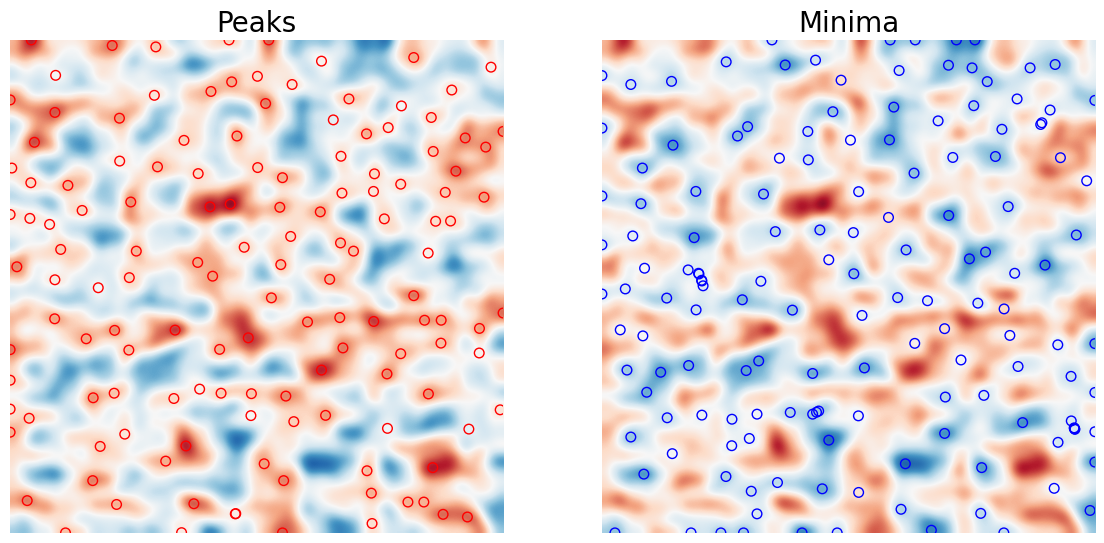
\includegraphics[width=0.8\textwidth]{figures/peaks_minima.png}
    \caption{Identification of peaks and minima in a smoothed convergence map. The left panel shows the smoothed convergence field $\kappa_{\mathrm{smooth}}(\hat{\mathbf{n}})$ with peaks (red circles) satisfying the peak condition (Equation~\eqref{eq:peak_condition}), and the right panel highlights the minima (blue circles) satisfying the minimum condition (Equation~\eqref{eq:min_condition}).}
    \label{fig:peak_min}
\end{figure}

\subsection{Peaks of Gaussian Random Fields}
For a Gaussian random field (GRF), the statistics of peaks and minima can be analytically derived. The expected number density of peaks above a threshold $\nu$ in a GRF is given by:
\begin{equation}
    N_{\mathrm{peak}}(\nu) = \frac{1}{(2\pi)^{3/2} R_*^3} e^{-\nu^2/2} \left[ \nu^2 - 1 \right],
    \label{eq:bbks_peak}
\end{equation}
where $\nu = \tilde{\kappa}_{\mathrm{smooth}}$, and $R_*$ is a characteristic scale defined by:
\begin{equation}
    R_*^2 = \frac{\langle |\nabla \kappa_{\mathrm{smooth}}|^2 \rangle}{\langle \kappa_{\mathrm{smooth}}^2 \rangle}.
    \label{eq:R_star}
\end{equation}
Similarly, the expected number density of minima below $-\nu$ is:
\begin{equation}
    N_{\mathrm{min}}(-\nu) = N_{\mathrm{peak}}(\nu).
    \label{eq:bbks_min}
\end{equation}

\begin{comment}
In particular, the local maxima
and minima on convergence maps are associated with massive haloes
and emptiest regions (voids) in our universe. The study of such
peaks and minima is highly sensitive to non-linear structures and a
complementary probe to constrain S8 (Liu et al. 2015a, b; Kacprzak
et al. 2016; Martinet et al. 2018; Shan et al. 2018; Coulton et al.
2020; Davies et al. 2021; Harnois-Deraps ´ et al. 2021; Davies et al.
2022; Zurcher ¨ et al. 2022; Liu et al. 2023).

measurements of peaks and
minima (Davies et al. 2022; Zürcher et al. 2022; Liu et al. 2023a;
Marques et al. 2024),
\end{comment}


\section{Minkowski Functionals}
\label{sec:minkowski_functionals}
Minkowski functionals are powerful morphological descriptors derived from integral geometry, widely used to quantify the geometry and topology of spatial structures in cosmological datasets. 
Here, we will review \citet{2010PhRvD..81h3505M}, \citet{2012PhRvD..85j3513K} and \citet{2013PhRvD..88l3002P} for a comprehensive understanding of Minkowski functionals and their applications in cosmology.

\subsection{Definition}
Given a two-dimensional random field $\kappa(\hat{\mathbf{n}})$ (in our case, the convergence field) with zero mean and variance $\kappa^2 = \sigma_0^2$, we can consider its excursion sets $\Sigma(\nu) = \{ \kappa > \nu \sigma_0 \}$ which consist of all the points at which the field exceeds a particular threshold value $\nu \sigma_0$. 
Figure~\ref{fig:excursion_sets} depicts the excursion sets $\Sigma(\nu) = \{ \kappa > \nu \sigma_0 \}$ of a two-dimensional convergence field $\kappa(\hat{\mathbf{n}})$, which is characterized by a zero mean and variance $\sigma_0^2$. The figure consists of four panels, each corresponding to an increasing threshold value of $\nu = 0.5, 1, 1.5,$ and $2$. As the threshold $\nu$ increases, the excursion sets progressively diminish in size and connectivity. 
\begin{figure}[ht]
    \centering
    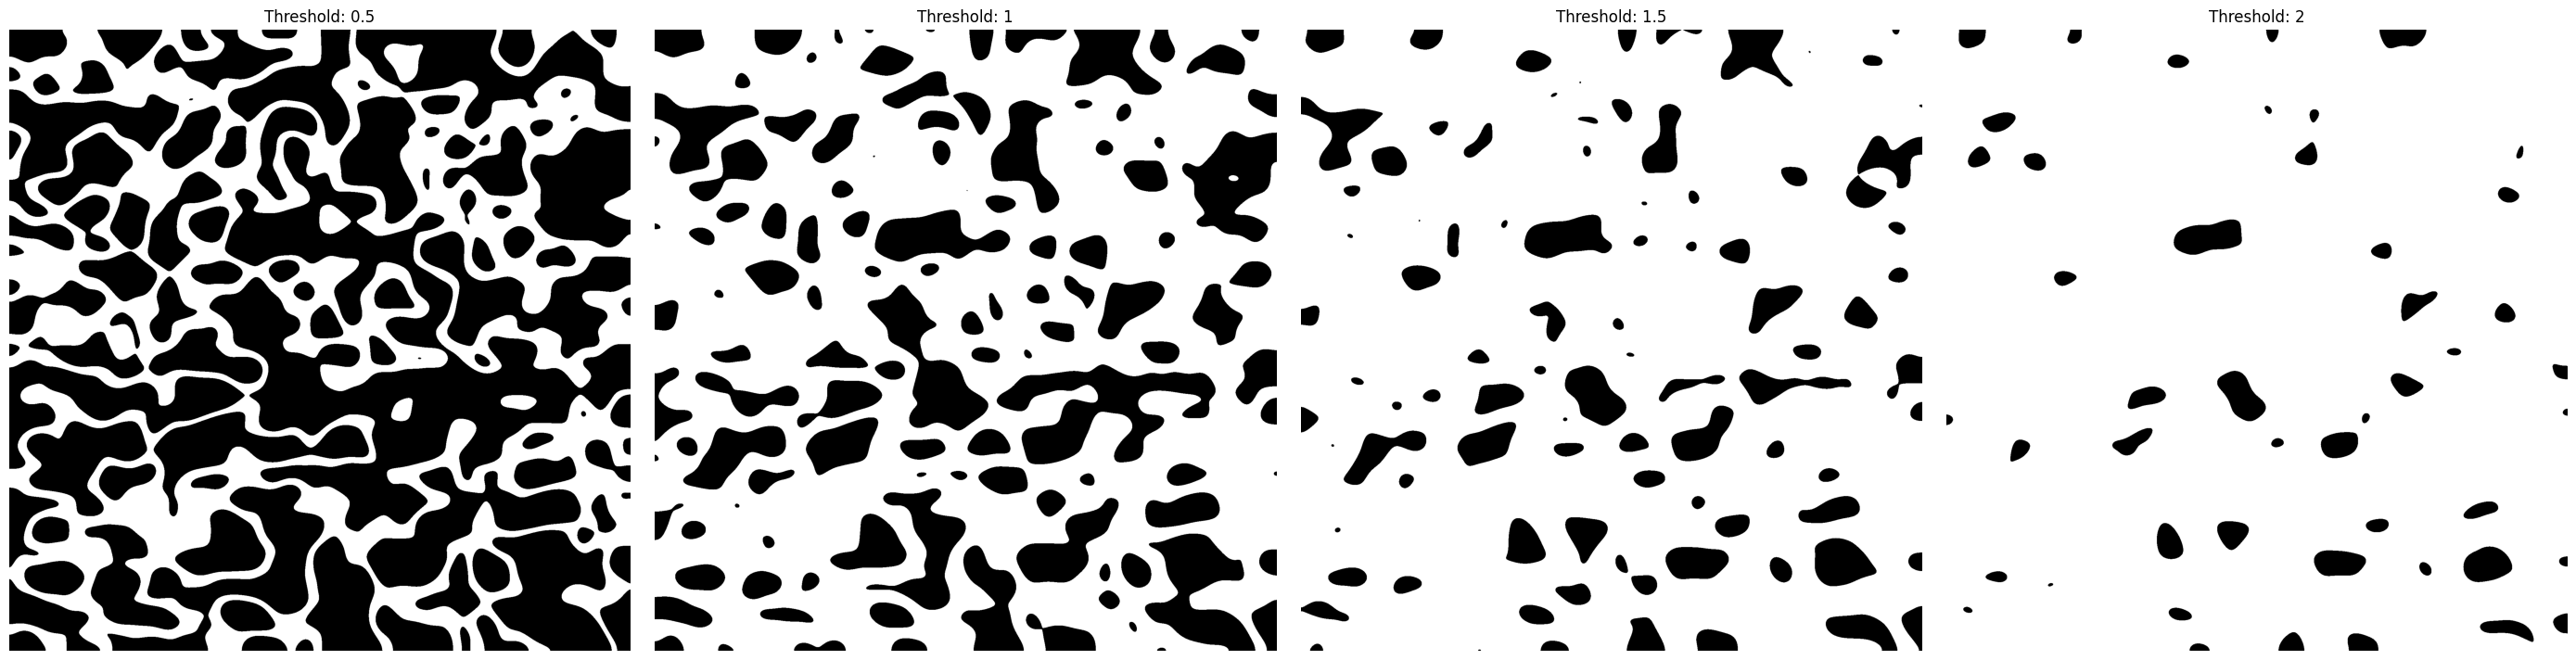
\includegraphics[width=\textwidth]{figures/threshold_comparison.png}
    \caption{Visualization of excursion sets $\Sigma(\nu) = \{ \kappa > \nu \sigma_0 \}$ of a two-dimensional random field $\kappa(\hat{\mathbf{n}})$, where $\kappa$ represents the convergence field with zero mean and variance $\sigma_0^2$. 
    Black regions correspond to regions where the field exceeds the threshold value $\nu \sigma_0$. The panels correspond to increasing threshold values ($\nu = 0.5, 1, 1.5, 2$), illustrating how the size and connectivity of the excursion sets change as the threshold increases.}
    \label{fig:excursion_sets}
\end{figure}
The three Minkowski functionals $V_0(\nu)$, $V_1(\nu)$, and $V_2(\nu)$ measure, respectively, the area, the length of the boundary, and the genus characteristic of these excursion sets:
\begin{align}
    V_0(\nu) &= \frac{1}{A} \int_{\Sigma(\nu)} \, da, \label{eq:minkowski_V0} \\
    V_1(\nu) &= \frac{1}{4A} \int_{\partial \Sigma(\nu)} \, dl, \label{eq:minkowski_V1} \\
    V_2(\nu) &= \frac{1}{2\pi A} \int_{\partial \Sigma(\nu)} \mathcal{K} \, dl, \label{eq:minkowski_V2}
\end{align}
where $A$ is the total area of the field, $da$ and $dl$ are the area and length elements, and $\mathcal{K}$ is the geodesic curvature along the boundary $\partial \Sigma(\nu)$. 

\subsection{Computation of Minkowski Functionals}
In practical applications, Minkowski functionals are computed numerically from discrete convergence maps.

For a given threshold $\nu$, the excursion set $\Sigma(\nu)$ is identified by:
\begin{equation}
    \Sigma(\nu) = \{ \hat{\mathbf{n}} \in S^2 \mid \tilde{\kappa}(\hat{\mathbf{n}}) > \nu \}, \label{eq:excursion_set_normalized}
\end{equation}
where $\tilde{\kappa} = (\kappa - \langle \kappa \rangle) / \sigma_0$ is the normalized convergence field.

Given a pixelized convergence map, the continuous integrals in Equations~\eqref{eq:minkowski_V0}--\eqref{eq:minkowski_V2} are approximated by discrete sums \citep{2012PhRvD..85j3513K}:
\begin{align}
    V_0(\nu) &\approx \frac{1}{N_{\mathrm{pix}}} \sum_{i=1}^{N_{\mathrm{pix}}} \Theta(\tilde{\kappa}_i - \nu), \label{eq:V0_discrete} \\
    V_1(\nu) &\approx \frac{1}{N_{\mathrm{pix}}} \sum_{i=1}^{N_{\mathrm{pix}}}  \delta_D(\tilde{\kappa}_i - \nu) \, \sqrt{\kappa_{, x}^2 + \kappa_{, y}^2}, \label{eq:V1_discrete} \\
    V_2(\nu) &\approx \frac{1}{N_{\mathrm{pix}}} \sum_{i=1}^{N_{\mathrm{pix}}}  \delta_D(\tilde{\kappa}_i - \nu) \, \frac{2\kappa_{, x}\kappa_{, y}\kappa_{, xy} - \kappa_{, x}^2 \kappa_{, yy} - \kappa_{, y}^2}{\kappa_{, xx}{\kappa_{, x}^2 + \kappa_{, y}^2}} \label{eq:V2_discrete}
\end{align}
where $\mathcal{N}(i)$ denotes the set of neighboring pixels to pixel $i$, and $\delta_D$ is the Dirac delta function. The first and second order derivatives $\kappa_{, x}$ etc., are approximated by finite differences.

\subsection{Minkowski Functionals in Gaussian Random Fields}
In the analysis of \emph{Gaussian random fields} (GRFs), Minkowski functionals provide a robust analytical framework for quantifying the morphological characteristics of the field's excursion sets. For a two-dimensional GRF \(\kappa(\hat{\mathbf{n}})\) with zero mean and variance \(\sigma_0^2\), the Minkowski functionals can be explicitly calculated and are given by \citep{2010PhRvD..81h3505M}:
\begin{align}
    V_0(\nu) &= \frac{1}{2}\left[1 - \mathrm{erf}\left( \frac{\nu}{\sqrt{2}\sigma_0} \right) \right], \label{eq:V0_GRF} \\
    V_1(\nu) &= \frac{1}{8\sqrt{2}} \frac{\sigma_1}{\sigma_0} \exp\left( -\frac{\nu^2}{2\sigma_0^2} \right), \label{eq:V1_GRF} \\
    V_2(\nu) &= \frac{\nu}{4\sqrt{2}} \frac{\sigma_1^2}{\sigma_0^3} \exp\left( -\frac{\nu^2}{2\sigma_0^2} \right), \label{eq:V2_GRF}
\end{align}
where \(\nu\) denotes the threshold level defining the excursion set, \(\mathrm{erf}\) is the error function, and \(\sigma_1^2 = \langle |\nabla \kappa|^2 \rangle = \langle \kappa_{, x}^2 + \kappa_{, y}^2 \rangle\) represents the variance of the gradient of the field. Here, \(V_0(\nu)\) corresponds to the area fraction of the excursion set, \(V_1(\nu)\) to the total boundary length per unit area, and \(V_2(\nu)\) to the Euler characteristic per unit area.

\begin{comment}
\subsection{Applications in Cosmology}
Minkowski functionals furnish an algebraic framework for quantifying the geometrical and topological properties of scalar fields \citep{1994A&A...288..697M}. In cosmology, they are instrumental in characterizing the intricate patterns formed by the large-scale structure of the Universe \citep{1996dmu..conf..281S, 1997ApJ...482L...1S}. These patterns, which trace the underlying matter distribution, are sensitive to higher-order statistical moments of the matter density field and thus provide insights beyond those accessible through two-point correlation functions \citep{2001ApJ...551L...5S}.

Recently, Minkowski functionals have been extensively employed in various cosmological investigations. They have been utilized to probe non-linear features in the CMB anisotropies \citep{2012JCAP...01..048L, 2016MNRAS.461.1363N, 2024JCAP...01..039C, 2024JCAP...05..076H}, to analyze anisotropies in the distribution of galaxies \citep{2003PASJ...55..911H, 2022ApJ...928..108A}, to constrain neutrino masses through their impact on the matter power spectrum \citep{2024MNRAS.528.4513M, 2023JCAP...09..037L}, and to test theories of modified gravity that predict deviations from General Relativity on cosmological scales \citep{2017MNRAS.466.2402S, 2024PhRvD.109h3537J}. Moreover, Minkowski functionals have emerged as a powerful and efficient probe for detecting primordial non-Gaussianity, as demonstrated in several studies \citep{2006ApJ...653...11H, 2008MNRAS.385.1613H, 2008MNRAS.389.1439H, 2012MNRAS.425.2187H, 2012ApJ...760...45S}.

In the realm of weak lensing, Minkowski functionals have been proposed as a method to break the degeneracy between the matter density parameter \(\Omega_m\) and the amplitude of matter fluctuations \(\sigma_8\) inherent in traditional two-point statistics \citep{2001ApJ...552L..89M}. Subsequent studies have leveraged Minkowski functionals applied to weak lensing convergence maps to extract cosmological information beyond that accessible through the power spectrum alone, thereby enhancing constraints on cosmological parameters \citep{2012PhRvD..85j3513K, 2013ApJ...774..111S, 2015PhRvD..91j3511P, 2022OJAp....5E..13G}.
\end{comment}

\chapter{Covariance}
The covariance matrix encapsulates the uncertainties and correlations between different measurements. It plays a critical role in parameter estimation techniques, including maximum likelihood analyses and Bayesian inference, and is foundational in forecasting the capabilities of future surveys through the Fisher information matrix.

The covariance matrix between two observables $\mathcal{O}_i$ and $\mathcal{O}_j$ is defined as:
\begin{equation}
    \mathrm{Cov}(\mathcal{O}_i, \mathcal{O}_j) = \left\langle (\mathcal{O}_i - \langle \mathcal{O}_i \rangle)(\mathcal{O}_j - \langle \mathcal{O}_j \rangle) \right\rangle,
\end{equation}
where $\langle \cdot \rangle$ denotes the ensemble average over multiple realizations.
For an unbiased estimator, the covariance matrix is given by:
\begin{equation}
    \label{eq:covariance}
    \mathrm{Cov}(\mathcal{O}_i, \mathcal{O}_j) = \frac{1}{N_{\mathrm{sim}} - 1} \sum_{n=1}^{N_{\mathrm{sim}}} (\mathcal{O}_i^{(n)} - \langle \mathcal{O}_i \rangle) (\mathcal{O}_j^{(n)} - \langle \mathcal{O}_j \rangle),
\end{equation}
where \( N_{\mathrm{sim}} \) is the number of simulations, and \( \mathcal{O}_i^{(n)} \) is the \( i \)-th realization of the statistic in the \( n \)-th simulation.

\section{Role of the Covariance Matrix}
Though we leave the Fisher forecast using the covariance matrix for future work, it is worthful to discuss the importance of the covariance matrix in the context of weak lensing statistics \citep{2004MNRAS.348..897T, 2005A&A...442...69K}. When comparing theoretical models to observational data, we often compute a likelihood function $\mathcal{L}(\mathbf{d} | \mathbf{p})$, where $\mathbf{d}$ represents the data vector and $\mathbf{p}$ denotes the set of cosmological parameters. For Gaussian-distributed data, the likelihood function is given by:
\begin{equation}
    \ln \mathcal{L}(\mathbf{d} | \mathbf{p}) = -\frac{1}{2}(\mathbf{d} - \mathbf{m}(\mathbf{p}))^{\mathrm{T}} \mathbf{C}^{-1} (\mathbf{d} - \mathbf{m}(\mathbf{p})) + \mathrm{const},
\end{equation}
where $\mathbf{m}(\mathbf{p})$ is the model prediction for the data vector $\mathbf{d}$, and $N$ is the number of data points. The covariance matrix $\mathbf{C}$ quantifies the uncertainties and correlations between different data points.

Based on the likelihood function, we can construct the Fisher information matrix $\mathcal{F}_{\alpha\beta}$, which quantifies the sensitivity of the likelihood function to changes in the model parameters $\mathbf{p}$. The Fisher information matrix is defined as:
\begin{equation}
    \mathcal{F}_{\alpha\beta} = -\left\langle \frac{\partial^2 \ln \mathcal{L}}{\partial p_\alpha \partial p_\beta} \right\rangle,
\end{equation}
In the case of Gaussian likelihoods, the Fisher information matrix is simplified to:
\begin{equation}
    \mathcal{F}_{\alpha\beta} = \frac{1}{2} \mathrm{Tr} \left[ \mathbf{C}^{-1} \frac{\partial \mathbf{C}}{\partial p_\alpha} \mathbf{C}^{-1} \frac{\partial \mathbf{C}}{\partial p_\beta} \right]\Bigg|_{p_\alpha = \mu_\alpha} + \left(\frac{\partial \mu}{\partial p_\alpha}\right)^{\mathrm{T}} \mathbf{C}^{-1} \frac{\partial \mu}{\partial p_\beta},
\end{equation}
where $\mathbf{\mu}$ is the mean of the data vector $\mathbf{d}$. The Fisher matrix allows us to forecast the expected uncertainties on the parameters via the Cramér-Rao bound:
\begin{equation}
    \left\langle (\Delta p_\alpha)^2 \right\rangle \geq (\mathcal{F}^{-1})_{\alpha\alpha},
\end{equation}
where $\Delta p_\alpha$ is the uncertainty on the $\alpha$-th parameter. Note that this condition is marginalized over all other parameters, $p_\beta$ ($\beta \neq \alpha$).

\section{Covariance of the Matter Power Spectrum}
Understanding the covariance matrix of the matter power spectrum \( P_m(k) \) is crucial before delving into two-dimensional weak lensing statistics. 
The covariance matrix for the matter power spectrum is defined as:
\begin{equation}
    \mathrm{Cov}(k, k') = \left\langle \hat{P}_m(k) \hat{P}_m(k') \right\rangle - \left\langle \hat{P}_m(k) \right\rangle \left\langle \hat{P}_m(k') \right\rangle,
\end{equation}
where \( \hat{P}_m(k) \) is an estimator of the matter power spectrum obtained from a finite volume \( V \).
An estimator for the matter power spectrum in a finite survey volume is given by \citep{1994ApJ...426...23F}:
\begin{equation}
    \hat{P}_m(k) = (2\pi)^3 \delta_D(\mathbf{k} + \mathbf{k'}) \tilde{\delta}(\mathbf{k}) \tilde{\delta}(-\mathbf{k}) = V_f \int_{V_s(k)} \frac{\mathrm{d}^3 \mathbf{k}}{V_s(k)} \, \tilde{\delta}(\mathbf{k}) \, \tilde{\delta}(-\mathbf{k}),
\end{equation}
where $V_f = (2\pi)^3 / V$ is the volume of a Fourier cell where $V$ is the total survey volume, and $V_s(k) = 4\pi k^2 \Delta k$ is the volume of the shell in Fourier space corresponding to wavenumber \( k \).

To derive the covariance matrix, we substitute the estimator \( \hat{P}_m(k) \) into the covariance definition:
\begin{equation}
    \mathrm{Cov}(\mathbf{k}, \mathbf{k'}) = V_f^2 \left( \left\langle \tilde{\delta}(\mathbf{k}) \tilde{\delta}(-\mathbf{k}) \tilde{\delta}(\mathbf{k'}) \tilde{\delta}(-\mathbf{k'}) \right\rangle - \left\langle \tilde{\delta}(\mathbf{k}) \tilde{\delta}(-\mathbf{k}) \right\rangle \left\langle \tilde{\delta}(\mathbf{k'}) \tilde{\delta}(-\mathbf{k'}) \right\rangle\right)
\end{equation}
The four-point correlation function \( \left\langle \tilde{\delta}(\mathbf{k}_1) \tilde{\delta}(\mathbf{k}_2) \tilde{\delta}(\mathbf{k}_3) \tilde{\delta}(\mathbf{k}_4) \right\rangle \) can be decomposed using Wick's theorem (valid for Gaussian fields) into products of two-point functions \citep{PhysRev.80.268}:
\begin{eqnarray}
    \left\langle \tilde{\delta}(\mathbf{k}) \tilde{\delta}(-\mathbf{k}) \tilde{\delta}(\mathbf{k'}) \tilde{\delta}(-\mathbf{k'}) \right\rangle 
    &=& \left\langle \tilde{\delta}(\mathbf{k}) \tilde{\delta}(-\mathbf{k}) \right\rangle \left\langle \tilde{\delta}(\mathbf{k'}) \tilde{\delta}(-\mathbf{k'}) \right\rangle \nonumber \\
    &+& \left\langle \tilde{\delta}(\mathbf{k}) \tilde{\delta}(\mathbf{k'}) \right\rangle \left\langle \tilde{\delta}(-\mathbf{k}) \tilde{\delta}(-\mathbf{k'}) \right\rangle \nonumber \\
    &+& \left\langle \tilde{\delta}(\mathbf{k}) \tilde{\delta}(-\mathbf{k'}) \right\rangle \left\langle \tilde{\delta}(-\mathbf{k}) \tilde{\delta}(\mathbf{k'}) \right\rangle \nonumber \\ 
    &+& \left\langle \tilde{\delta}(\mathbf{k}) \tilde{\delta}(-\mathbf{k}) \tilde{\delta}(\mathbf{k'}) \tilde{\delta}(-\mathbf{k'}) \right\rangle_c,
\end{eqnarray}
where the last term represents the connected (non-Gaussian) part of the four-point function, known as the trispectrum \( T(\mathbf{k}, -\mathbf{k}, \mathbf{k}', -\mathbf{k}') \).

Using the properties of the Dirac delta function and assuming statistical isotropy, the covariance matrix simplifies to:
\begin{equation}
    \mathrm{Cov}(k, k') = \frac{2 P_m(k)^2}{N(k)} \delta_{k,k'} + \frac{T(k, k')}{V}
\end{equation}
where \( N(k) = V_s(k) / V_f \) is the number of independent modes in the shell at wavenumber \( k \). The first term represents the Gaussian (disconnected) contribution, and the second term accounts for the non-Gaussian (connected) contribution from the trispectrum.

In the presence of a finite survey volume, super-sample covariance arises due to modes larger than the survey size influencing the observed modes \citep{PhysRevD.87.123504}. This effect adds an additional term to the covariance matrix:
\begin{equation}
    \mathrm{Cov}(k, k') = \frac{2 P_m^2(k)}{N(k)} \delta_{kk'} + \frac{1}{V} T(k, k') + \left( \frac{\partial P_m(k)}{\partial \delta_b} \right) \left( \frac{\partial P_m(k')}{\partial \delta_b} \right) \sigma_b^2,
\end{equation}
where \( \delta_b \) represents the large-scale (background) density fluctuation, and \( \sigma_b^2 \) is its variance:
\begin{equation}
    \sigma_b^2 = \int \frac{\mathrm{d}^3 k}{(2\pi)^3} P_m(k) |\tilde{W}(\mathbf{k})|^2,
\end{equation}
with \( \tilde{W}(\mathbf{k}) \) being the Fourier transform of the survey window function \( W(\mathbf{x}) \).
The derivatives \( \partial P_m(k) / \partial \delta_b \) quantify the response of the power spectrum to changes in the background density and can be related to the concept of the response function or integrated perturbation theory \citep{2014PhRvD..89h3519L}.

\section{Covariance of the Angular Power Spectrum}
We consider a cosmological survey characterized by a window function \( W(\boldsymbol{\theta}) \) and a total survey area \( A \), defined as the integral of the window function over the sky \citep{PhysRevD.87.123504}:
\begin{equation}
    A = \int \mathrm{d}^2 \theta \, W(\boldsymbol{\theta}).
\end{equation}
The window function \( W(\boldsymbol{\theta}) \), and its Fourier transform, \( \tilde{W}(\boldsymbol{\ell}) \), accounts for the survey geometry and selection effects. 

In the presence of the window function, the estimator for the angular power spectrum \( C_\ell \) is given by \citep{PhysRevD.87.123504}:
\begin{equation}
    \hat{C}_\ell = \frac{1}{A} \int_{A_\ell} \frac{\mathrm{d}^2 \ell'}{A_\ell} \int \frac{\mathrm{d}^2 q_1}{(2\pi)^2} \int \frac{\mathrm{d}^2 q_2}{(2\pi)^2} \, \tilde{W}(\mathbf{q}_1) \tilde{W}(\mathbf{q}_2) \, \tilde{\kappa}(\boldsymbol{\ell}' - \mathbf{q}_1) \, \tilde{\kappa}(-\boldsymbol{\ell}' - \mathbf{q}_2),
\end{equation}
where \( \tilde{\kappa}(\boldsymbol{\ell}) \) is the Fourier transform of the convergence field \( \kappa(\boldsymbol{\theta}) \), and \( A_\ell \) is the area of the annulus in Fourier space corresponding to multipole \( \ell \), defined as:
\begin{equation}
    A_\ell = \int_{|\boldsymbol{\ell}| = \ell} \mathrm{d}^2 \boldsymbol{\ell} \approx 2 \pi \ell \Delta \ell, \quad (\Delta \ell / \ell \ll 1),
\end{equation}
with \( \Delta \ell \) being the width of the multipole bin. The integrals over \( \mathbf{q}_1 \) and \( \mathbf{q}_2 \) incorporate the effects of the survey window function, effectively convolving the true sky signal with the survey geometry.

The covariance matrix of the angular power spectrum \( C_\ell \) is defined as:
\begin{equation}
    \mathrm{Cov}(\ell_1, \ell_2) = \left\langle \hat{C}_{\ell_1} \hat{C}_{\ell_2} \right\rangle - \left\langle \hat{C}_{\ell_1} \right\rangle \left\langle \hat{C}_{\ell_2} \right\rangle,
\end{equation}
which measures the statistical correlation between estimates of \( C_{\ell_1} \) and \( C_{\ell_2} \).
Substituting the estimator \( \hat{C}_\ell \) into the covariance definition and expanding the resulting expression leads to terms involving two-point and four-point correlation functions of the convergence field \( \kappa(\boldsymbol{\theta}) \). Specifically, the covariance can be expressed as:
\begin{equation}
    \mathrm{Cov}(\ell_1, \ell_2) = \frac{1}{A^2} \int_{A_{\ell_1}} \frac{\mathrm{d}^2 \ell_1'}{A_{\ell_1}} \int_{A_{\ell_2}} \frac{\mathrm{d}^2 \ell_2'}{A_{\ell_2}} \left[ \left\langle \tilde{\kappa}(\boldsymbol{\ell}_1') \tilde{\kappa}(-\boldsymbol{\ell}_1') \tilde{\kappa}(\boldsymbol{\ell}_2') \tilde{\kappa}(-\boldsymbol{\ell}_2') \right\rangle - \left\langle \tilde{\kappa}(\boldsymbol{\ell}_1') \tilde{\kappa}(-\boldsymbol{\ell}_1') \right\rangle \left\langle \tilde{\kappa}(\boldsymbol{\ell}_2') \tilde{\kappa}(-\boldsymbol{\ell}_2') \right\rangle \right].
\end{equation}
The first term inside the brackets involves the four-point correlation function (connected and disconnected parts), while the second term is the product of two-point correlation functions. After evaluating the integrals and applying the appropriate approximations, the covariance matrix for the angular power spectrum \( C_\ell \) simplifies to:
\begin{equation}
    \mathrm{Cov}(\ell_1, \ell_2) = \frac{1}{A} \left[ \frac{(2\pi)^2}{A_\ell} C_{\ell_1}^2 \delta_{\ell_1, \ell_2} +  \tilde{\mathcal{T}}^W_{\ell_1, \ell_2} \right],
\end{equation}
where \( \tilde{\mathcal{T}}^W_{\ell_1, \ell_2} \) is the windowed (or convolved) trispectrum, incorporating the effects of the finite survey window.

Using the Limber approximation \citep{1954ApJ...119..655L}, which simplifies the projection of three-dimensional quantities into two dimensions, the covariance matrix can be related to the matter power spectrum. The trispectrum can be decomposed using the trispectrum consistency relation, allowing the covariance matrix to be written as:
\begin{equation}
    \mathrm{Cov}(\ell_1, \ell_2) = \mathrm{Cov}^{G}(\ell_1, \ell_2) + \mathrm{Cov}^{\text{NG}}(\ell_1, \ell_2) + \mathrm{Cov}^{\mathrm{SSC}}(\ell_1, \ell_2),
\end{equation}
where:
\begin{align}
    \mathrm{Cov}^{G}(\ell_1, \ell_2) &= \frac{1}{A} \frac{(2\pi)^2}{A_\ell} C_{\ell_1}^2 \delta_{\ell_1, \ell_2},\\
    \mathrm{Cov}^{\text{NG}}(\ell_1, \ell_2) &= \frac{1}{A} \int_{A_{\ell_1}} \frac{\mathrm{d}^2 \ell_1'}{A_{\ell_1}} \int_{A_{\ell_2}} \frac{\mathrm{d}^2 \ell_2'}{A_{\ell_2}} \, T(\boldsymbol{\ell}_1', -\boldsymbol{\ell}_1', \boldsymbol{\ell}_2', -\boldsymbol{\ell}_2'),\\
    \mathrm{Cov}^{\mathrm{SSC}}(\ell_1, \ell_2) &= \frac{1}{A^2} \int_0^{\chi_s} \frac{\mathrm{d} \chi}{\chi^6} W^4(\chi) \, \frac{\partial P_{m}(k_1)}{\partial \delta_b} \frac{\partial P_{m}(k_2)}{\partial \delta_b} \sigma_b^2,
\end{align}
Notably, the super-sample covariance term \( \mathrm{Cov}^{\mathrm{SSC}}(\ell_1, \ell_2) \) arises from the large-scale density fluctuations modulating the observed power spectrum within the survey area \citep{PhysRevD.87.123504}.

\section{Covariance of Higher-Order Statistics}
Despite some successes in analytical modeling (\citealt{2018PhRvD..97d3532C, 2018A&A...611A..83L, 2019A&A...624A..61L, 2023OJAp....6E...1U}), computing the covariance matrices for higher-order statistics  still need to rely on simulations. Drawing an analogy with the matter power spectrum, the covariance matrix for higher-order statistics can be expressed as:
\begin{equation}
    \mathrm{Cov}(\mathcal{O}_i, \mathcal{O}_j) = \mathrm{Cov}^{\mathrm{noSSC}}(\mathcal{O}_i, \mathcal{O}_j) + \mathrm{Cov}^{\mathrm{SSC}}(\mathcal{O}_i, \mathcal{O}_j),
\end{equation}
A rigorous super-sample covariance for line-of-sight integrated observable $\mathcal{O}_i$, where $\mathcal{O}_i = \int dV_i \mathfrak{o}_i = \int \chi_i^2 d\chi \mathfrak{o}_i$, is given by \citep{2016JCAP...08..005L}:
\begin{equation}
    \mathrm{Cov}^{\mathrm{SSC}}(\mathcal{O}_i, \mathcal{O}_j) = 
    \iint \mathrm{d}V_i \, \mathrm{d}V_j \,
    \left(
        \frac{\partial \mathfrak{o}_i}{\partial \delta_b}
    \right)
    \left(
        \frac{\partial \mathfrak{o}_j}{\partial \delta_b}
    \right)
    \sigma_b^2, 
\end{equation}

\chapter{Surveys(Make it shorter)}
\section{Introduction to Astronomical Surveys}

\subsection{Purpose and Scientific Objectives}
Contemporary astronomical surveys constitute extensive and systematic observational endeavors designed to map and catalog vast regions of the sky with unparalleled depth and precision. These surveys yield comprehensive datasets that are crucial for addressing fundamental questions in astrophysics and cosmology. They facilitate investigations into the elusive nature of \emph{dark energy}, provide rigorous tests of the \emph{standard cosmological model}—the $\Lambda$CDM paradigm—and enable detailed studies of the formation and evolution of \emph{cosmic structures}. By delivering high-fidelity observational data, these surveys significantly advance our understanding of the Universe and the fundamental physical laws that govern it.

\paragraph{Testing the Standard Cosmological Model}
One of the primary objectives of astronomical surveys is to rigorously test the standard cosmological model, known as the $\Lambda$CDM model (Lambda Cold Dark Matter). While the $\Lambda$CDM model successfully accounts for a wide range of cosmological observations~\cite{Planck2018}, it encounters notable challenges such as the \emph{Hubble tension}—a significant discrepancy between measurements of the Universe's expansion rate derived from early-universe observations~\cite{Planck2018} and those obtained from late-universe observations~\cite{Riess2019}—and inconsistencies in parameters like the amplitude of matter clustering, denoted by $S_8$~\cite{Heymans2021}. These surveys endeavor to produce precise measurements of cosmological parameters, aiming to either corroborate the $\Lambda$CDM model or uncover deviations that could indicate new physics beyond the current paradigm. By juxtaposing high-precision observational data with theoretical predictions, astronomical surveys enhance our understanding of the fundamental forces and constituents that shape the cosmos.

\paragraph{Studying the Growth and Evolution of Cosmic Structures}
Another fundamental objective of astronomical surveys is to investigate the formation and evolution of cosmic structures, including galaxies, galaxy clusters, and dark matter halos. By mapping the spatial distribution of millions of galaxies, these surveys construct detailed maps of dark matter over vast cosmological volumes. Techniques such as \emph{weak gravitational lensing}—which measures subtle distortions in the shapes of background galaxies caused by the gravitational potential of intervening mass distributions—illuminate the role of dark matter in the process of structure formation~\cite{Bartelmann2001}. Moreover, \emph{galaxy-galaxy lensing}, which correlates the lensing signal with the positions of foreground galaxies, provides insights into the connection between luminous matter and the underlying dark matter distribution~\cite{Mandelbaum2017}. These comprehensive maps enable stringent tests of theoretical predictions from various cosmological models regarding the large-scale structure of the Universe.

\subsection{Imaging vs.\ Spectroscopic Surveys}
Astronomical surveys can be broadly categorized into \emph{imaging surveys} and \emph{spectroscopic surveys}, each employing distinct methodologies to capture and analyze celestial phenomena.

\subsubsection{Imaging Surveys}
Imaging surveys acquire wide-field images of the sky across multiple wavelengths, providing spatial data that enable astronomers to map cosmic structures, identify transient events, and analyze galaxy populations. By systematically scanning large regions of the sky, these surveys generate extensive catalogs documenting object positions, apparent magnitudes, and morphological characteristics. The varying depths and angular resolutions of these surveys facilitate the detection of both nearby and distant astronomical objects, thereby supporting detailed morphological and statistical studies across cosmic time. Prominent examples of imaging surveys include the \textit{Sloan Digital Sky Survey} (SDSS; \citealt{2019BAAS...51g.274K}), the \textit{Dark Energy Survey} (DES; \citealt{2018ApJS..239...18A}), and the forthcoming \textit{Legacy Survey of Space and Time} (LSST; \citealt{2019ApJ...873..111I}).

\subsubsection{Spectroscopic Surveys}

Spectroscopic surveys collect detailed spectral data from individual celestial objects by dispersing their emitted light into constituent wavelengths, thereby revealing redshifts, chemical compositions, and kinematic properties. These measurements are indispensable for studying galaxy dynamics, the distribution of dark matter, and the expansion history of the Universe. Unlike imaging surveys that capture broad swaths of the sky, spectroscopic surveys often target specific objects identified in imaging data, focusing on obtaining high-resolution spectral information. The spectral resolution and wavelength coverage are critical parameters that determine the precision of measurements such as redshift determinations and elemental abundances. Key spectroscopic surveys include the \textit{Baryon Oscillation Spectroscopic Survey} (BOSS; \citealt{2013AJ....145...10D}), which investigates baryon acoustic oscillations, the \textit{Dark Energy Spectroscopic Instrument} (DESI; \citealt{2016arXiv161100036D}), designed to map large-scale cosmic structure, and the \textit{Kilo-Degree Survey} (KiDS; \citealt{2013Msngr.154...44D}) with its spectroscopic extensions that enhance research on dark matter and dark energy.

\subsection{Ground-Based vs.\ Space-Based Surveys}

The operational platform of an astronomical survey—whether ground-based or space-based—fundamentally determines its observational capabilities, including wavelength coverage, angular resolution, and sensitivity.

\subsubsection{Ground-Based Surveys}
Ground-based surveys utilize telescopes located on Earth's surface, capitalizing on accessible infrastructure and enabling routine maintenance and upgrades of large, high-power instruments. These observatories can host a diverse array of instruments designed for observations across multiple wavelengths and facilitate prompt follow-up observations. However, atmospheric effects such as absorption, scattering, and turbulence degrade image quality and restrict observations at certain wavelengths, particularly in the ultraviolet and infrared regions. Notable ground-based surveys include the \emph{Hyper Suprime-Cam} (HSC; \citealt{2018PASJ...70S...4A}), the \emph{Dark Energy Survey} (DES; \citealt{2018ApJS..239...18A}), and the \emph{Kilo-Degree Survey} (KiDS; \citealt{2013Msngr.154...44D}).

\subsubsection{Space-Based Surveys}
Space-based surveys operate from satellites or space telescopes positioned above Earth's atmosphere, offering exceptional clarity and sensitivity across a wide range of wavelengths, especially in the ultraviolet and infrared bands that are largely inaccessible from the ground. Free from atmospheric distortions, these instruments achieve high angular resolution and can detect faint, distant objects through long-duration, stable observations. Despite these advantages, space missions are costly, require extensive international collaboration, and present limited opportunities for maintenance, upgrades, or repairs. Prominent examples include the \emph{Hubble Space Telescope} (HST; \citealt{2001ApJ...553...47F}), the forthcoming \emph{Nancy Grace Roman Space Telescope} (\emph{Roman}; \citealt{2015arXiv150303757S}), and the \emph{Gaia} mission~\citep{2016A&A...595A...2G}.

\subsection{Stage-III vs.\ Stage-IV Surveys}
\label{sec:survey-stages}

The classification of astronomical surveys into \emph{Stage-III} and \emph{Stage-IV} categories serves to distinguish successive generations based on technological sophistication, scale, and scientific objectives. While this framework is particularly pertinent in dark energy research~\cite{2006astro.ph..9591A}, it is broadly applicable across cosmology and astrophysics.

\subsubsection{Stage-III Surveys}
Stage-III surveys represent the current generation of large-scale astronomical projects, integrating advanced yet moderately scaled instrumentation and methodologies. Their primary aims include refining cosmological parameters, mapping large-scale structures, and deepening our understanding of dark energy and dark matter. Utilizing multi-band imaging and spectroscopy, Stage-III surveys achieve moderate sky coverage and depth, supported by sophisticated data processing pipelines capable of handling substantial datasets. Notable examples of Stage-III surveys include the \emph{Dark Energy Survey} (DES; \citealt{2018ApJS..239...18A}), the \emph{Kilo-Degree Survey} (KiDS; \citealt{2013Msngr.154...44D}), and the \emph{Hyper Suprime-Cam} survey (HSC; \citealt{2018PASJ...70S...4A}), all of which have provided high-quality data instrumental in advancing cosmological models.

\subsubsection{Stage-IV Surveys}
Stage-IV surveys represent the forthcoming generation of astronomical initiatives, characterized by unparalleled scale, depth, and precision. Leveraging cutting-edge technologies, these surveys aim to achieve high-precision cosmological measurements, explore dark energy and dark matter with greater fidelity, and uncover new astrophysical phenomena. They are distinguished by ultra-wide sky coverage, deep imaging and spectroscopy, high angular resolution, and the integration of multi-wavelength data. Advanced data management techniques are employed to process petabyte-scale datasets efficiently. Prominent examples include the \emph{Legacy Survey of Space and Time} (LSST) conducted by the Vera C.\ Rubin Observatory~\cite{2019ApJ...873..111I}, the \emph{Dark Energy Spectroscopic Instrument} (DESI; \citealt{2016arXiv161100036D}), and the forthcoming \emph{Nancy Grace Roman Space Telescope} (\emph{Roman}; \citealt{2015arXiv150303757S}), all of which are poised to transform our understanding of the cosmos and address critical questions in astrophysics.

\section{Subaru Hyper Suprime-Cam}

\subsection{Instrument Overview}

The \emph{Subaru Hyper Suprime-Cam} (HSC; \citealt{2018PASJ...70S...1M}) is a state-of-the-art wide-field imaging instrument mounted at the prime focus of the 8.2-meter Subaru Telescope located on Maunakea, Hawaii. The HSC features an expansive $1.5^\circ$ diameter field of view, achieved through an array of 104 charge-coupled devices (CCDs), each with $2048 \times 4096$ pixels, culminating in a total of approximately 870 megapixels. This sophisticated configuration enables the acquisition of high-fidelity, wide-field optical data, augmented by a precision corrector lens system that preserves image quality across the entire observational field. The substantial field of view, combined with Subaru's significant light-collecting capabilities, renders the HSC exceptionally well-suited for deep and wide imaging surveys that are critical for studies of \emph{weak gravitational lensing} and the \emph{large-scale structure} of the Universe.

The instrument is equipped with five broad-band filters—\textit{g}, \textit{r}, \textit{i}, \textit{z}, and \textit{y} (\citealt{2018PASJ...70...66K})—alongside several narrow-band filters that cover optical to near-infrared wavelengths. Benefiting from the exceptional atmospheric conditions at Maunakea and the high-resolution optics of the Subaru Telescope, the HSC achieves a median seeing of $0.6$ arcseconds in the $i$-band, facilitating detailed and precise astronomical analyses.

\subsection{Survey Design: The Hyper Suprime-Cam Subaru Strategic Program}

The \emph{Hyper Suprime-Cam Subaru Strategic Program} (HSC-SSP; \citealt{2018PASJ...70S...4A}) is a comprehensive, multi-band imaging survey that exploits the advanced capabilities of the HSC instrument. Initially allocated 300 observing nights over a five-year period starting in March 2014, the program's duration was extended to 340 nights to compensate for observational losses due to weather conditions, technical issues, and seismic activity. The HSC-SSP is meticulously designed to address a broad spectrum of astrophysical inquiries, including but not limited to cosmology, galaxy evolution, and solar system science.

The survey is stratified into three distinct layers, each engineered to achieve specific scientific objectives through varying degrees of sky coverage and imaging depth:

\begin{itemize}
    \item \textbf{Wide Layer}: Encompassing approximately 1,400 square degrees around the celestial equator, the Wide layer attains a depth of $i \sim 26$ magnitudes. This extensive coverage is optimized for mapping large-scale structures and conducting statistical studies of weak gravitational lensing, thereby contributing significantly to our understanding of dark matter distribution and cosmic acceleration.

    \item \textbf{Deep Layer}: Covering roughly 28 square degrees across four distinct fields, the Deep layer reaches a depth of $i \sim 27$ magnitudes. This intermediate configuration balances area and depth, supporting research on galaxy evolution, supernova detection, and the statistical properties of faint astronomical objects.

    \item \textbf{UltraDeep Layer}: Targeting two fields that collectively cover 3.5 square degrees, the UltraDeep layer achieves an impressive depth of $i \sim 28$ magnitudes. Utilizing both broad-band and narrow-band filters, this layer is dedicated to probing the high-redshift Universe, facilitating investigations into early galaxy formation, quasars, and the epoch of reionization, thereby providing critical insights into the early phases of cosmic evolution.
\end{itemize}

\subsection{Data Releases and Processing}

To date, the HSC-SSP has disseminated several public data releases—DR1, DR2, and DR3 (\citealt{2018PASJ...70S...8A, 2019PASJ...71..114A, 2022PASJ...74..247A})—each incorporating progressively larger datasets, enhanced calibration procedures, and refined data processing methodologies. The data processing pipeline is managed using the \emph{Legacy Survey of Space and Time} (LSST) Science Pipelines, which provide high-quality analysis tools accessible to the astronomical community. These tools generate calibrated imaging data, comprehensive photometric catalogs, and advanced data products such as photometric redshifts and precise shape measurements. Consequently, the HSC-SSP data releases empower a wide array of scientific investigations and promote collaborative advancements within the field of astronomy.

\section{Dark Energy Survey}

\subsection{Overview and Objectives}

The \emph{Dark Energy Survey} (DES; \citealt{2005astro.ph.10346T, 2018ApJS..239...18A, 2021ApJS..255...20A}) was meticulously designed as a comprehensive, wide-field imaging survey operating in optical and near-infrared wavelengths, with the primary objective of probing the nature of cosmic acceleration and the underlying mechanism of \emph{dark energy}. Spanning approximately $5{,}000$ square degrees of the Southern Galactic Cap, DES was conducted over a six-year period from August 2013 to January 2019. The survey utilized the $570$-megapixel \emph{Dark Energy Camera} (DECam; \citealt{2015AJ....150..150F}), which is mounted on the 4-meter \emph{Blanco Telescope} at the Cerro Tololo Inter-American Observatory (CTIO) in Chile.

\subsection{Survey Components}

DES observations were strategically divided into two primary components: the \emph{Wide-Area Survey} and the \emph{Supernova Survey}, each meticulously tailored to address specific scientific goals within the overarching framework of DES.

\subsubsection{Wide-Area Survey}

The Wide-Area Survey constituted the principal observational effort of DES, covering approximately $5{,}000$ square degrees across five photometric bands ($g$, $r$, $i$, $z$, $Y$). This extensive footprint was purposefully selected to overlap with other significant surveys, such as the \emph{South Pole Telescope Survey} and the \emph{Sloan Digital Sky Survey} (SDSS) Stripe 82~\cite{2009ApJS..182..543A}, thereby enhancing calibration accuracy and enabling synergistic cross-survey analyses. The Wide-Area Survey aimed to map the large-scale structure of the Universe with high precision, facilitating studies on galaxy clustering, weak gravitational lensing, and the abundance of galaxy clusters, all of which are sensitive probes of dark energy and cosmological parameters.

\subsubsection{Supernova Survey}

Complementing the Wide-Area Survey, the Supernova Survey focused on a more concentrated region of approximately $27$ square degrees. This component employed a higher observational cadence, with images acquired in the $g$, $r$, $i$, and $z$ bands roughly every seven days. Such a cadence was specifically designed to capture transient phenomena, notably \emph{Type Ia supernovae}~\cite{2019PhRvL.122q1301A}, which serve as standard candles for cosmic distance measurements. By monitoring these supernovae over time, the Supernova Survey aimed to construct a Hubble diagram extending to high redshifts, thereby providing stringent constraints on the equation of state of dark energy.

\subsection{Instrumentation and Data Processing}

DECam, the instrument central to DES, features a focal plane array of 62 science CCDs, each with $2048 \times 4096$ pixels, providing a large field of view of $2.2$ degrees in diameter. The camera's design includes specialized optics to achieve uniform image quality across the field, essential for weak lensing measurements that require precise shape determinations of distant galaxies.

Data processing for DES was handled by the \emph{DES Data Management} (DESDM) system~\cite{2008SPIE.7016E..0LM}, which performed tasks ranging from image detrending and astrometric calibration to co-addition and catalog generation. Advanced algorithms were employed for photometric calibration, object detection, and classification, ensuring high-quality data products suitable for cosmological analyses.

\subsection{Scientific Contributions}

DES has made significant contributions to cosmology and astrophysics, including precise measurements of cosmic shear~\cite{2022PhRvD.105b3514A} and galaxy clustering~\cite{2022PhRvD.105b3520A}. The combination of these probes has led to improved constraints on cosmological parameters, particularly the matter density $\Omega_m$ and the amplitude of matter fluctuations $\sigma_8$. Furthermore, DES data have been instrumental in addressing tensions in cosmological measurements, such as the $S_8$ discrepancy, and in exploring possible extensions to the $\Lambda$CDM model.


\section{Legacy Survey of Space and Time}

\subsection{Overview and Scientific Objectives}

The \emph{Legacy Survey of Space and Time} (LSST; \citealt{2009arXiv0912.0201L, 2019ApJ...873..111I}), conducted by the Vera C.\ Rubin Observatory, is a groundbreaking optical survey meticulously designed to perform a comprehensive imaging campaign covering approximately half of the celestial sphere. Operating with six photometric filters (\emph{ugrizy}), LSST will systematically re-image its surveyed regions at intervals of a few nights over a planned ten-year observational period. This extensive survey is anticipated to produce an unparalleled dataset, comprising approximately $3.2 \times 10^{13}$ individual observations of around $2 \times 10^{10}$ galaxies, along with a comparable number of stellar objects. This vast repository of observations will enable a broad spectrum of scientific investigations, including studies in cosmology, Galactic structure, and time-domain astrophysics.

\subsection{Instrumentation and Survey Strategy}

To achieve its ambitious scientific objectives, LSST has been constructed as an advanced, wide-field observatory centered around an 8.4-meter primary mirror and a field of view spanning 9.6 square degrees. The system's observational capabilities are enhanced by a 3.2-gigapixel camera, facilitating high-throughput data acquisition. The unique optical design employs a three-mirror system to deliver a wide field of view with excellent image quality across the entire focal plane.

The survey primarily employs a \emph{deep-wide-fast} observing strategy, allocating approximately 90\% of the telescope's operational time to this primary mode~\cite{2009arXiv0912.0201L}. This approach aims to maximize both spatial coverage and temporal cadence across the main survey region, enabling the detection of transient phenomena and the mapping of large-scale structures. The remaining 10\% of LSST's observing time is dedicated to specialized programs designed to address specific astrophysical phenomena. These programs include \emph{deep drilling fields}, which involve intensified observations in selected regions to achieve greater depth, and targeted surveys of dynamically complex areas, such as the Galactic plane. These tailored observational approaches are integral to fulfilling LSST's broader scientific mandate, offering critical data to complement the primary survey and enabling detailed analyses of both local and distant astronomical phenomena.

\subsection{Scientific Impact}

LSST is expected to make transformative contributions across multiple domains of astrophysics. In cosmology, it will provide precise measurements of dark energy parameters through studies of weak gravitational lensing, supernovae, baryon acoustic oscillations, and large-scale structure~\cite{2012arXiv1211.0310L}. In the study of the Milky Way, LSST will map the distribution and kinematics of stars, facilitating investigations into the Galaxy's formation history and structure~\cite{2019NatRP...1..450R}. The time-domain capabilities of LSST will enable the discovery and monitoring of transient and variable objects, such as supernovae, variable stars, and potentially hazardous near-Earth objects~\cite{2018Icar..303..181J}. Furthermore, LSST's extensive dataset will be invaluable for probing fundamental physics, such as testing general relativity on cosmological scales and searching for signatures of new physics beyond the Standard Model.

\section{Nancy Grace Roman Space Telescope}

\subsection{Overview and Mission Objectives}

The \emph{Nancy Grace Roman Space Telescope} (hereafter referred to as \emph{Roman}; formerly designated as the \emph{Wide-Field Infrared Survey Telescope}, \textit{WFIRST}; \citealt{2015arXiv150303757S}) represents a seminal endeavor within NASA's astrophysics portfolio. This mission leverages a 2.4-meter aperture telescope, originally developed for national reconnaissance purposes, repurposing its advanced instrumentation and observational capabilities toward forefront astronomical research. The \emph{Roman} mission is designed to address key questions in cosmology and exoplanet science, thereby significantly enhancing our understanding of the Universe's expansion history, the distribution of dark matter and dark energy, and the prevalence of planetary systems in our galaxy.

\subsection{Surveys and Scientific Goals}

The \emph{Roman} Space Telescope's scientific program is anchored by two primary surveys: the \emph{High Latitude Survey} and the \emph{Galactic Bulge Time Domain Survey}, each meticulously designed to achieve specific scientific objectives.

\subsubsection{High Latitude Survey}

A cornerstone of the \emph{Roman}'s scientific agenda is the \textbf{High Latitude Survey}, engineered to probe the enigmatic phenomenon of dark energy, which is hypothesized to drive the accelerated expansion of the Universe~\cite{1998AJ....116.1009R, 1999ApJ...517..565P}. This survey integrates a tripartite observational strategy to examine both the temporal evolution of cosmic expansion and the growth of large-scale structures. The employed methodologies encompass:

\begin{itemize}
    \item \textbf{Supernova Surveys}: Utilizing Type Ia supernovae as standard candles to trace the expansion history of the Universe~\cite{2011ApJ...737..102S}.
    \item \textbf{Weak Gravitational Lensing Imaging}: Mapping the distribution of dark matter through the subtle distortions of background galaxies~\cite{2001PhR...340..291B}.
    \item \textbf{Spectroscopic Surveys of Baryon Acoustic Oscillations}: Measuring the scale of baryon acoustic oscillations to serve as a cosmological standard ruler~\cite{2005ApJ...633..560E}.
\end{itemize}

These techniques collectively furnish a comprehensive understanding of the Universe's expansion history, thereby elucidating the properties and dynamics of dark matter and dark energy. The High Latitude Survey is anticipated to cover thousands of square degrees, providing high-resolution imaging and spectroscopy in the near-infrared wavelengths.

\subsubsection{Galactic Bulge Time Domain Survey}

Complementing the High Latitude Survey, the \textbf{Galactic Bulge Time Domain Survey} employs the microlensing technique to detect and characterize a substantial population of exoplanets, including those with masses as low as that of Mars~\cite{2019ApJS..241....3P}. Focusing on stellar populations within the Milky Way's bulge, this survey enhances our comprehension of planetary formation and distribution mechanisms in environments with high stellar density. By monitoring millions of stars over time, the \emph{Roman} Space Telescope aims to detect the gravitational microlensing events caused by planets orbiting both luminous and dark host stars, thus expanding the demographic census of exoplanets~\cite{2012ARA&A..50..411G}.

\subsection{Instrumentation and Capabilities}

The \emph{Roman} Space Telescope is equipped with a 2.4-meter primary mirror, comparable in size to the \emph{Hubble Space Telescope}, but with a significantly larger field of view—approximately 100 times greater~\cite{2015arXiv150303757S}. The primary instruments include:

\begin{itemize}
    \item \textbf{Wide Field Instrument (WFI)}: A near-infrared imager and spectrometer that provides high-resolution imaging and integral-field spectroscopy over a large field of view.
    \item \textbf{Coronagraph Instrument}: A technology demonstration instrument designed to perform high-contrast imaging and spectroscopy of exoplanets and circumstellar disks.
\end{itemize}

These advanced instruments enable the \emph{Roman} Space Telescope to perform wide-field surveys with unprecedented sensitivity and resolution in the near-infrared regime.

\subsection{Expected Scientific Contributions}

The \emph{Roman} Space Telescope is poised to make transformative contributions to astrophysics and cosmology. In addition to its primary surveys, it will offer opportunities for a \emph{Guest Observer} program, allowing the broader scientific community to propose observations for a wide range of astrophysical phenomena~\cite{2019arXiv190205569A}. The mission is expected to:

\begin{itemize}
    \item Provide precise measurements of cosmological parameters, refining our understanding of dark energy and the geometry of the Universe~\cite{2018ApJ...867...23H}.
    \item Expand the census of exoplanets, particularly those in the outer regions of planetary systems, thereby informing models of planetary formation and evolution~\cite{2019ApJS..241....3P}.
    \item Advance the study of galaxy formation and evolution through deep imaging and spectroscopy of distant galaxies~\cite{2018MNRAS.477.5382B}.
    \item Enhance our understanding of the Milky Way's structure and stellar populations~\cite{2020AJ....160..123J}.
\end{itemize}

By addressing these fundamental questions, the \emph{Roman} Space Telescope will significantly augment our knowledge of the cosmos and lay the groundwork for future astronomical discoveries.


\chapter{Simulations}
\section{Introduction to Numerical Simulations in Cosmology}
Numerical simulations are crucial in physics and astronomy for studying complex systems of interacting particles, such as galaxies and the Universe's large-scale structure, where analytical solutions are often impractical due to complexity and nonlinearity \citep{1981csup.book.....H, 1985ApJS...57..241E, 2005Natur.435..629S, 2005MNRAS.364.1105S}. This section provides an overview of $N$-body simulations commonly used in cosmology.

\subsection{Dark Matter-Only vs. Hydrodynamical Simulations}
In cosmology and astrophysics, simulation can be grouped into two main categories: dark matter-only simulations and hydrodynamical simulations. 

Dark matter simulations are used to study the large-scale structure of the universe, the formation of dark matter halos, and the evolution of dark matter particles under the influence of gravity. Since dark matter is effectively collisionless and interacts primarily through gravity, it can be modeled as a collection of particles that evolve under the influence of gravitational forces \citep{1985ApJS...57..241E}. 

Hydrodynamical simulations, on the other hand, include the effects of gas dynamics, star formation, and feedback processes from supernovae and active galactic nuclei (AGN) \citep{1989ApJS...70..419H, 2005Natur.435..629S, 2005MNRAS.364.1105S}. These simulations are more computationally expensive and require additional physics beyond gravity, such as hydrodynamics, radiative transfer, and chemistry.

\subsection{Historical Evolution and Growth in Particle Number}
Since the 1980s, numerical cosmology has developed algorithms to mitigate the computational challenges posed by long-range gravitational interactions by reducing global communication across the computational domain. Key algorithms include mesh-based methods, tree codes, and multipole expansions~\citep{1981csup.book.....H}. Figure~\ref{fig:particle-count} displays the number of particles used in selected $N$-body simulations employing these techniques. Symbols and colors indicate the gravitational solvers: particle-particle-particle-mesh (P$^3$M) and adaptive P$^3$M (AP$^3$M); parallel or vectorized P$^3$M; Tree codes; TreePM; and particle-mesh methods with adaptive mesh refinement (PM AMR).

Advancements in algorithms and software optimization have increased the number of particles in cosmological simulations beyond what direct summation methods allow. Since 1990, gravity-only simulations have exhibited a super-exponential growth trend, indicated by the quadratic regression in Figure~\ref{fig:particle-count}, reflecting significant methodological innovations beyond hardware improvements~\citep{leclercq2020}.

\begin{figure} \centering 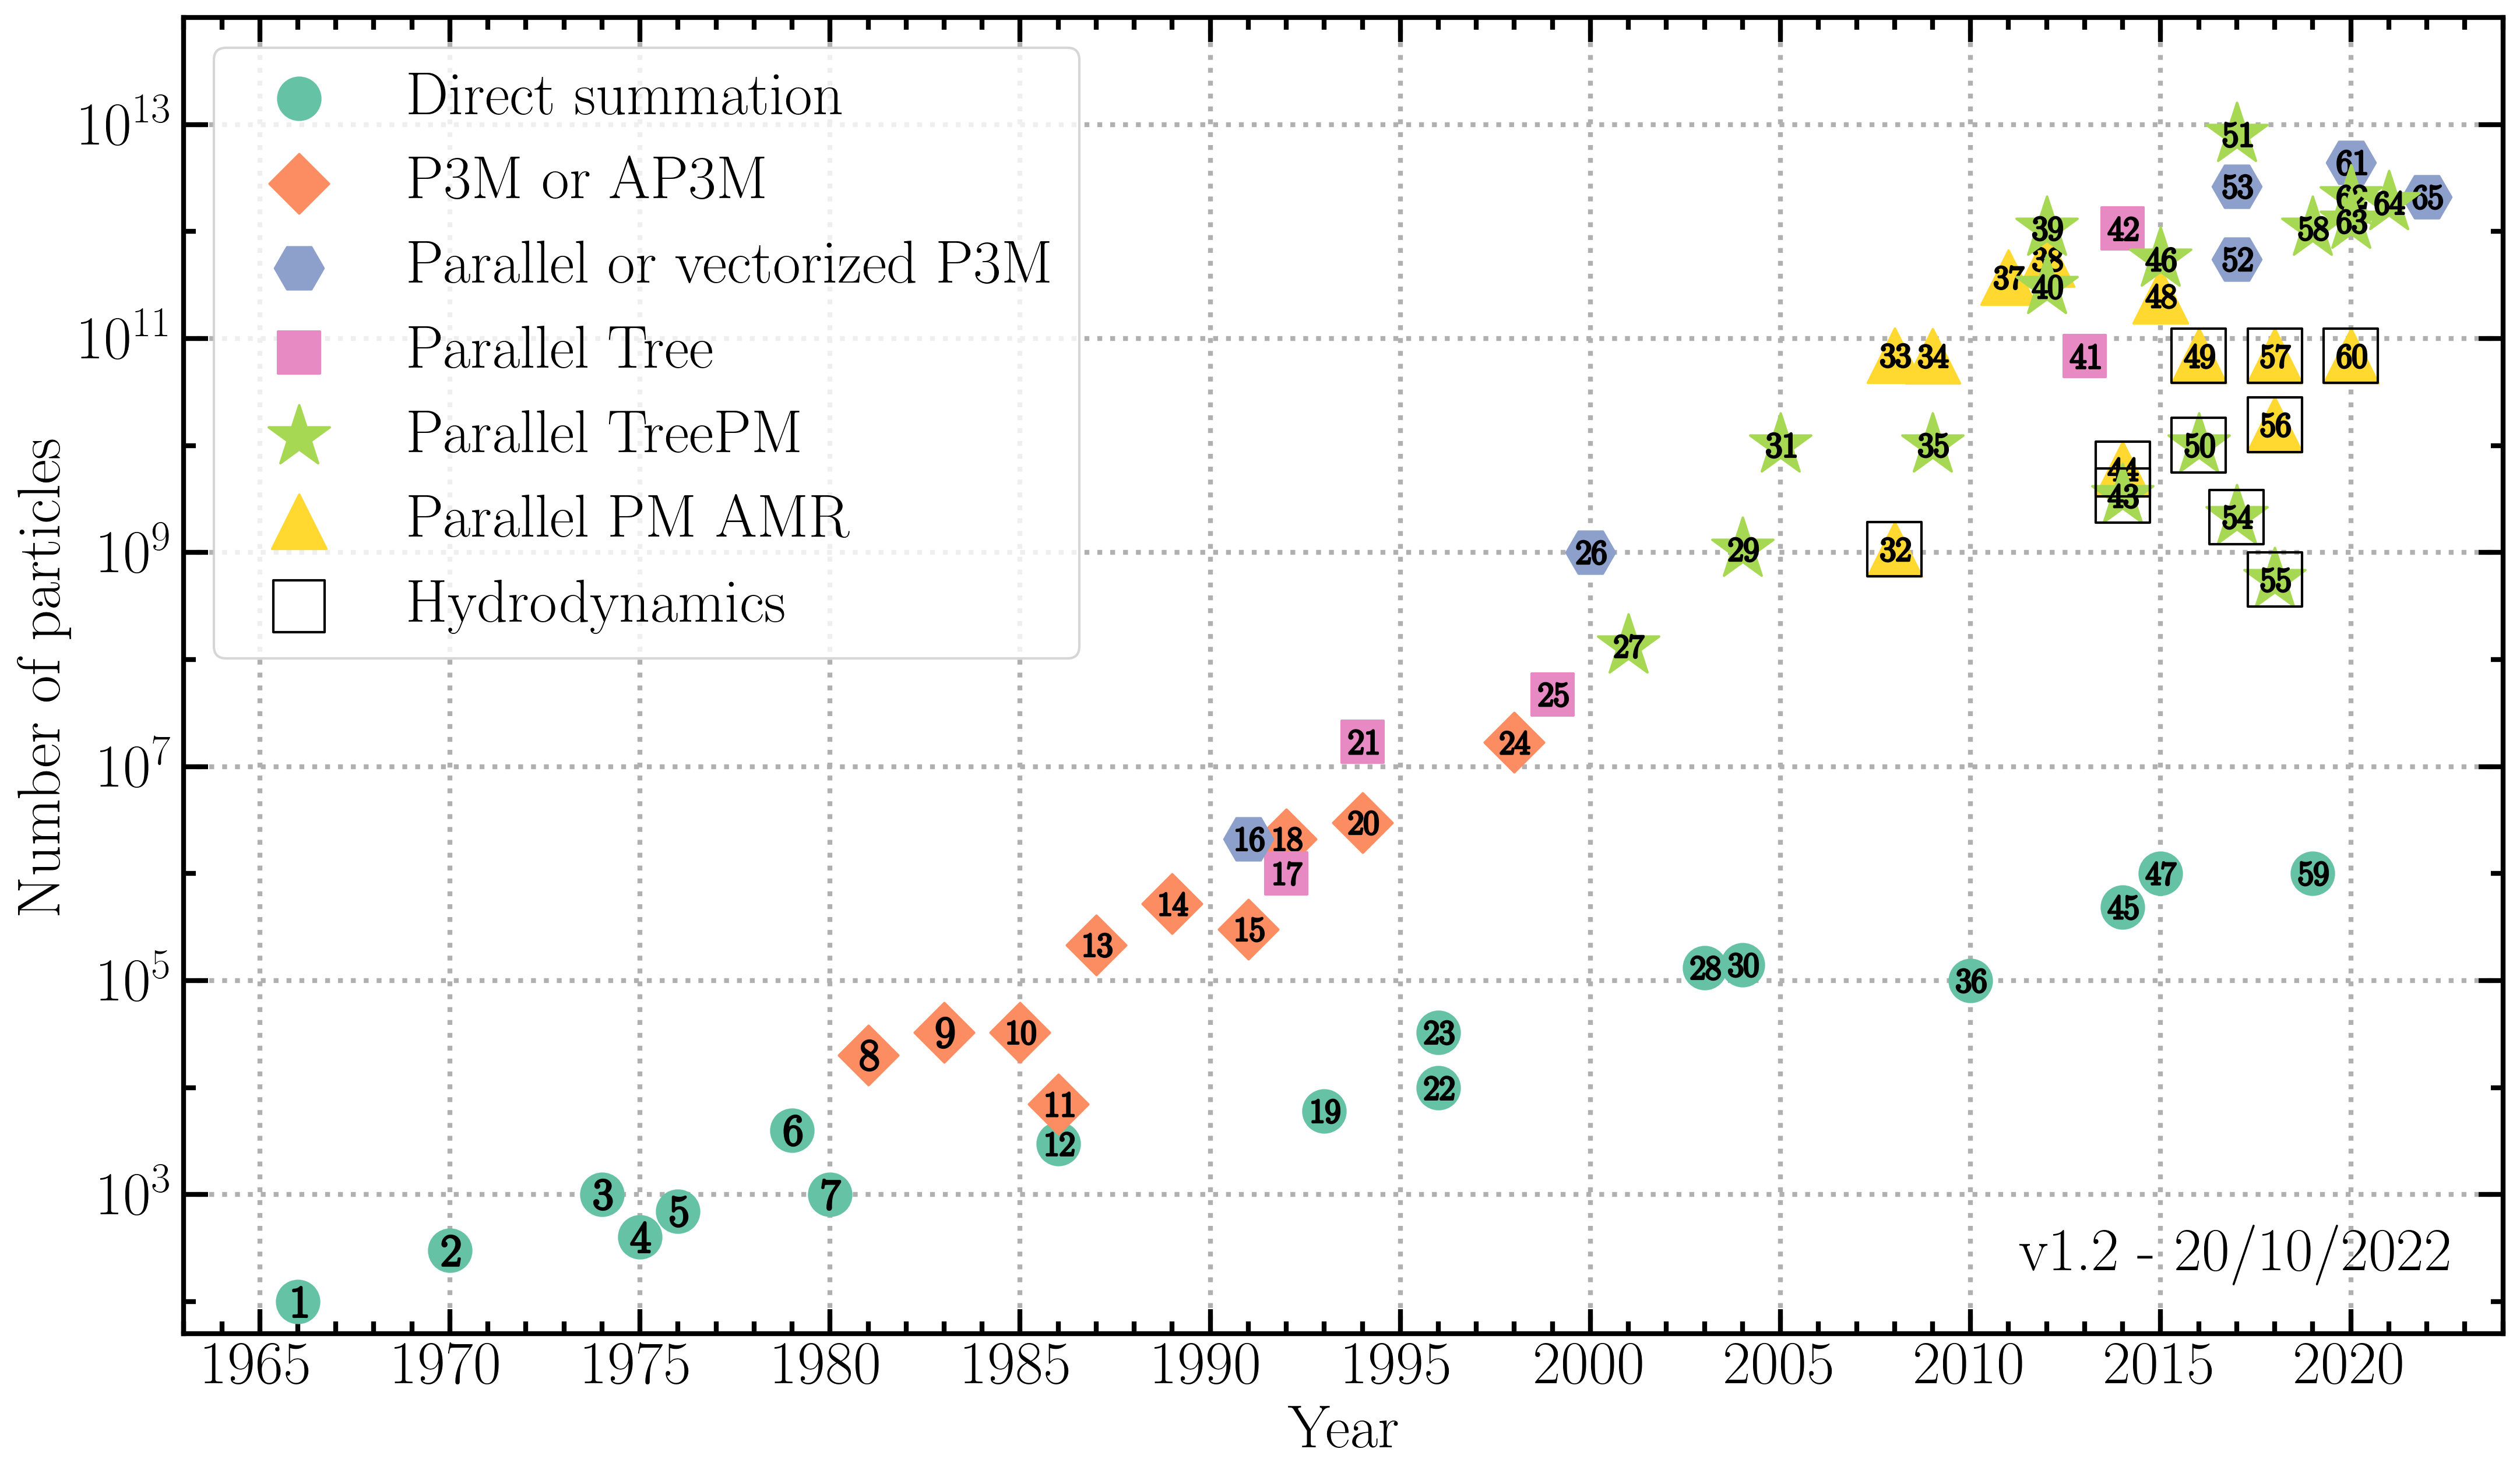
\includegraphics[width=\textwidth]{figures/Moore_law_cosmosims.png} \caption[Evolution of the number of particles used in $N$-body simulations]{Evolution of the number of particles used in $N$-body simulations as a function of the year of publication~\citep{leclercq2020}. The symbols and colors indicate the gravitational solver employed: P$^3$M and adaptive P$^3$M (AP$^3$M); parallel or vectorized P$^3$M; Tree codes; TreePM; and particle-mesh methods with adaptive mesh refinement (PM AMR). Hydrodynamic simulations are represented by black squares.} \label{fig:particle-count} \end{figure}

\section{Initial Condition Generation}
As we have seen in Section~\ref{sec:initial_conditions}, the primodial power spectrum $P(k)$ is a key ingredient in generating initial conditions for cosmological simulations. Based on the linear power spectrum, we will review the process of generating initial conditions for $N$-body simulations.

\subsection{Initial Density Field}
To generate the initial density field for the simulations, we express the density contrast $\delta(\mathbf{x})$ in terms of its Fourier components:
\begin{equation}
    \delta(\mathbf{x}) = \int \frac{d^3k}{(2\pi)^3} \tilde{\delta}(\mathbf{k}) e^{i\mathbf{k} \cdot \mathbf{x}}.
\end{equation}
Assuming a Gaussian random field, each Fourier mode $\tilde{\delta}(\mathbf{k})$ is a complex Gaussian random variable with zero mean and variance $P(k)$:
\begin{align}
    \tilde{\delta}(\mathbf{k}) &= A(\mathbf{k}) + i B(\mathbf{k}), \\
    \langle A(\mathbf{k}) \rangle &= \langle B(\mathbf{k}) \rangle = 0, \\
    \langle A(\mathbf{k}) A(\mathbf{k}') \rangle &= \langle B(\mathbf{k}) B(\mathbf{k}') \rangle = \frac{1}{2} P(k) \delta_D(\mathbf{k} - \mathbf{k}'), \\
    \langle A(\mathbf{k}) B(\mathbf{k}') \rangle &= 0,
\end{align}
where $A(\mathbf{k})$ and $B(\mathbf{k})$ are real Gaussian random variables, and $\delta_D$ is the Dirac delta function.

\subsection{Initial Displacement Field}
The initial displacement field $\boldsymbol{\Psi}(\mathbf{q})$ relates the Lagrangian coordinates $\mathbf{q}$ to the Eulerian coordinates $\mathbf{x}$:
\begin{equation}
    \mathbf{x}(\mathbf{q}) = \mathbf{q} + \boldsymbol{\Psi}(\mathbf{q}).
\end{equation}
The displacement field is proportional to the gradient of the gravitational potential $\Phi(\mathbf{q})$:
\begin{equation}
    \boldsymbol{\Psi}(\mathbf{q}) = - \nabla \Phi(\mathbf{q}),
\end{equation}
where the potential satisfies Poisson's equation:
\begin{equation}
    \nabla^2 \Phi(\mathbf{q}) = \delta(\mathbf{q}).
\end{equation}
The first order solution to the displacement field is given by the Zel'dovich approximation \citep{1970A&A.....5...84Z}:
\begin{align}
    -k^2 \tilde{\Phi}(\mathbf{k}) &= \tilde{\delta}(\mathbf{k}), \\
    \tilde{\boldsymbol{\Psi}}(\mathbf{k}) &= i \mathbf{k} \tilde{\Phi}(\mathbf{k}) = i \mathbf{k} \frac{\tilde{\delta}(\mathbf{k})}{k^2}, \\
    \boldsymbol{\Psi}(\mathbf{q}) &= \int \frac{d^3k}{(2\pi)^3} i \mathbf{k} \frac{\tilde{\delta}(\mathbf{k})}{k^2} e^{i\mathbf{k} \cdot \mathbf{q}}.
\end{align}

\subsection{Initial Velocities}
The initial velocities of particles are derived from the time derivative of the displacement field. The velocities are given by \citep{1985ApJS...57..241E}:
\begin{align}
    \mathbf{v}(\mathbf{q}) &= a H f(a) \boldsymbol{\Psi}(\mathbf{q}), \\
    \tilde{\mathbf{v}}(\mathbf{k}) &= a H f(a) \tilde{\boldsymbol{\Psi}}(\mathbf{k}) = a H f(a) i \mathbf{k} \frac{\tilde{\delta}(\mathbf{k})}{k^2}, \\
    \mathbf{v}(\mathbf{q}) &= i a H f(a) \int \frac{d^3k}{(2\pi)^3} \frac{\mathbf{k}}{k^2} \tilde{\delta}(\mathbf{k}) e^{i\mathbf{k} \cdot \mathbf{q}},
\end{align}
where $a$ is the scale factor, $H$ is the Hubble parameter, and $f(a)$ is the growth rate defined as:
\begin{equation}
    f(a) = \frac{d\ln D}{d\ln a},
\end{equation}

\section[N-Body Simulation Methods]{N-Body Simulation Methods: An Overview}
We outline the fundamental concepts and algorithms used in $N$-body simulations, including direct summation, particle-mesh methods, particle-particle particle-mesh (P3M) methods, and tree-particle-mesh (Tree-PM) methods.

Table~\ref{tab:simulation-methods} summarizes the key features of these methods, including computational complexity and example objectives they are best suited for.

\begin{table}[ht]
    \centering
    \begin{tabular}{lccc}
        \toprule
        \textbf{Method} & \textbf{Complexity} & \textbf{Objective} & \textbf{Key Features} \\
        \midrule
        Direct Summation & $\mathcal{O}(N^2)$ & Globular Clusters & Accurate, computationally intensive \\
        PM & $\mathcal{O}(N + M \log M)$ & Large-Scale Structure & Fast, smooths small-scale forces \\
        P3M & $\mathcal{O}(N \log N)$ & Large-Scale Structure & Combines direct summation and PM \\
        Tree-PM & $\mathcal{O}(N \log N)$ & Large-Scale Structure & Tree algorithm for short-range forces \\
        \bottomrule
    \end{tabular}
    \caption{Comparison of $N$-body simulation methods}
    \label{tab:simulation-methods}
\end{table}

\subsection{Direct Summation}
Direct Summation calculates gravitational forces between all particle pairs directly, scaling as $\mathcal{O}(N^2)$ and becoming computationally intensive for large $N$. 
Therefore, direct summation is typically used for small systems like globular clusters, where accuracy is paramount \citep{2015MNRAS.450.4070W, 2019MNRAS.484.3279P}.
Each particle $i$ has position $\mathbf{r}_i$, velocity $\mathbf{v}_i$, and mass $m_i$. At each time step $t$:
\begin{enumerate}
    \item \textbf{Compute Forces:}
    \[
    \mathbf{F}_i = G m_i \sum_{\substack{j=1 \\ j \neq i}}^{N} \frac{m_j (\mathbf{r}_j - \mathbf{r}_i)}{\|\mathbf{r}_j - \mathbf{r}_i\|^3}
    \]
    
    \item \textbf{Update Particle States:}
    \[
    \mathbf{v}_i(t + \Delta t) = \mathbf{v}_i(t) + \frac{\mathbf{F}_i}{m_i} \Delta t, \quad \mathbf{r}_i(t + \Delta t) = \mathbf{r}_i(t) + \mathbf{v}_i(t + \Delta t) \Delta t
    \]
    
    \item \textbf{Advance Time:}
    \[
    t \leftarrow t + \Delta t
    \]
\end{enumerate}

\subsection{Particle-Mesh (PM) Method} \label{sec:pm-method}
The PM method approximates gravitational forces by mapping particles onto a grid and solving for the gravitational potential, reducing computational cost to $\mathcal{O}(N + M \log M)$, where $M$ is the number of grid points. Combining with Adaptive Mesh Refinement (AMR), PM simulations can achieve high resolution in regions of interest while maintaining efficiency so that it is used in Hydrodynamical simulations recently \citep{2018MNRAS.475..676S, 2021A&A...653A.154T}.
The main difference between the PM method and direct summation is the grid-based force calculation:
\begin{enumerate}
    \item \textbf{Assign Particles to Grid:} See Section~\ref{sec:mass-assignment}.
    \item \textbf{Compute Density Field:}
    \[
    \rho(\mathbf{x}) = \sum_i m_i W(\mathbf{x} - \mathbf{r}_i) \quad \text{(where $W$: Interpolation Kernel)}
    \]
    \item \textbf{Solve Poisson's Equation:}
    \[
    \nabla^2 \Phi = 4\pi G \rho
    \]
    \item \textbf{Compute Force due to Potential:}
    \[
    \mathbf{E} = -\nabla \Phi
    \]
\end{enumerate}

\subsection{Particle-Particle Particle-Mesh (P3M) Method}
The P$^3$M method combines direct summation for short-range forces with the PM approach for long-range interactions, achieving $\mathcal{O}(N \log N)$ complexity while enhancing accuracy for nearby particles. Due to its balance between accuracy and efficiency, the P$^3$M (or the Adaptive P$^3$M \citep{1991ApJ...368L..23C}) method is widely used in hydrodynamical simulations \citep{1995ApJ...452..797C, 2002A&A...385..337T}.

Key parameters include mesh size, softening parameter $\epsilon$, and force resolution.

The difference between the P$^3$M method and the PM method lies in the force calculation:
\begin{enumerate}
    \item \textbf{Long-Range Forces (PM):}
    \[
    \mathbf{F}_{\text{long},i} = m_i \mathbf{E}_{\text{long}}(\mathbf{r}_i)
    \]
    \item \textbf{Short-Range Forces (Direct Summation):}
    \begin{enumerate}[label={(\alph*)}]
        \item \textbf{Neighbor Search:}
        Identify particles $j$ within cutoff radius $r_{\text{cut}}$ of particle $i$.
        \item \textbf{Force Calculation:}
        \[
        \mathbf{F}_{\text{short},i} = -G m_i \sum_{\substack{j \in \text{neighbors}}} \frac{m_j (\mathbf{r}_i - \mathbf{r}_j)}{\left(\|\mathbf{r}_i - \mathbf{r}_j\|^2 + \epsilon^2\right)^{3/2}}
        \]
    \end{enumerate}
    \item \textbf{Combine Forces:}
    \[
    \mathbf{F}_i = \mathbf{F}_{\text{long},i} + \mathbf{F}_{\text{short},i}
    \]
\end{enumerate}

\subsection{Tree-Particle-Mesh (Tree-PM) Method}
The Tree-PM method integrates the PM approach for long-range forces with a tree algorithm for short-range interactions, reducing complexity to $\mathcal{O}(N \log N)$ \citep{1986Natur.324..446B}. Several popular simulations such as Illustris \citep{2014MNRAS.444.1518V} and EAGLE \citep{2015MNRAS.446..521S, 2015MNRAS.450.1937C, 2017arXiv170609899T} use the Tree-PM method.
Proper tuning of parameters like grid size, softening length $\epsilon$, and opening angle $\theta_{\text{max}}$ is essential.

The main updates in the Tree-PM method compared to the P$^3$M method are in the tree construction when calculating short-range forces:
\begin{enumerate}
    \item \textbf{Tree Construction:}
    \begin{enumerate}[label={(\alph*)}]
        \item \textbf{Build Spatial Cells:}
        Partition the simulation volume into spatial cells (e.g., octree) and assign particles to nodes.
        \item \textbf{Multipole Moments:}
        For each node $j$, calculate mass $M_j$ and center of mass $\mathbf{r}_{\text{cm},j}$.
    \end{enumerate}
    \item \textbf{Force Calculation:}
    For each particle $i$, traverse the tree to compute the short-range gravitational force:
        \[
        \mathbf{F}_{\text{short},i} = -G m_i \sum_{\text{nodes}} \frac{M_j (\mathbf{r}_i - \mathbf{r}_j)}{(\|\mathbf{r}_i - \mathbf{r}_j\|^2 + \epsilon^2)^{3/2}}
        \]
        using the opening angle criterion:
        \[
        \theta = \frac{l_j}{\|\mathbf{r}_i - \mathbf{r}_j\|} < \theta_{\text{max}}
        \]
        where $l_j$ is the size of node $j$ and $\theta_{\text{max}}$ is the maximum allowed opening angle.
\end{enumerate}

\section{Computational Tools and Optimization Techniques}
Efficient computational tools are crucial for large-scale simulations and data analysis in scientific and engineering applications. This section overviews key computational techniques and algorithms used in $N$-body simulations and large-scale structure studies.

\subsection{Fast Fourier Transforms (FFT)}
The Fast Fourier Transform (FFT) is a highly efficient algorithm for computing the Discrete Fourier Transform (DFT) of a sequence. Given a sequence of $N$ complex numbers $\{x_n\}_{n=0}^{N-1}$, the DFT is defined as:
\begin{equation}
    X_k = \sum_{n=0}^{N-1} x_n e^{-2\pi i kn / N}, \quad k = 0, 1, \dots, N-1.
\end{equation}
The naive computation of the DFT requires $\mathcal{O}(N^2)$ operations. The FFT reduces this complexity to $\mathcal{O}(N \log N)$ by exploiting the symmetry and periodicity properties of the exponential kernel. The most common FFT algorithm is the Cooley-Tukey radix-2 FFT \citep{d3ea2d52-5ab2-3128-8b80-efb85267295d}, which recursively decomposes the DFT into smaller DFTs of even and odd-indexed elements:
\begin{align}
    X_k &= \sum_{n=0}^{N/2-1} x_{2n} e^{-2\pi i k (2n) / N} + \sum_{n=0}^{N/2-1} x_{2n+1} e^{-2\pi i k (2n+1) / N} \\
         &= X_k^{\text{even}} + e^{-2\pi i k / N} X_k^{\text{odd}},
\end{align}
where $X_k^{\text{even}}$ and $X_k^{\text{odd}}$ are the DFTs of the even and odd subsequences, respectively.

\subsection{Mass Assignment Schemes}\label{sec:mass-assignment}
Mass assignment schemes map particle masses onto a computational grid to compute density fields and gravitational forces, ensuring mass conservation and minimizing aliasing errors. Common schemes include:
\begin{itemize}
    \item \textbf{Nearest Grid Point (NGP):} Each particle is assigned entirely to the nearest grid point.
    \item \textbf{Cloud-In-Cell (CIC):} Mass is linearly interpolated to the nearest $2^3 = 8$ surrounding grid points.
    \item \textbf{Triangular-Shaped Cloud (TSC):} Mass is distributed to the nearest $3^3 = 27$ grid points using a quadratic interpolation function.
\end{itemize}
In Fourier space, these mass assignment window functions are represented as:
\begin{equation}
    W(\mathbf{k}) = \prod_{i=1}^{3} W(k_i),
\end{equation}
where
\begin{equation}
    W(k_i) = \left[\frac{\sin\left(\pi k_i / (2 k_N)\right)}{\pi k_i / (2 k_N)}\right]^p,
\end{equation}
with $k_N$ being the Nyquist wavenumber, $k_i$ the $i$-th component of the wavevector $\mathbf{k}$, and $p = 1$ for NGP, $p = 2$ for CIC, and $p = 3$ for TSC \citep{1981csup.book.....H, 1985ApJS...57..241E}.

Figure~\ref{fig:mass-assignment} illustrates the mass assignment process for a particle distribution on a 1D grid using different schemes.
\begin{figure}[ht]
    \centering
    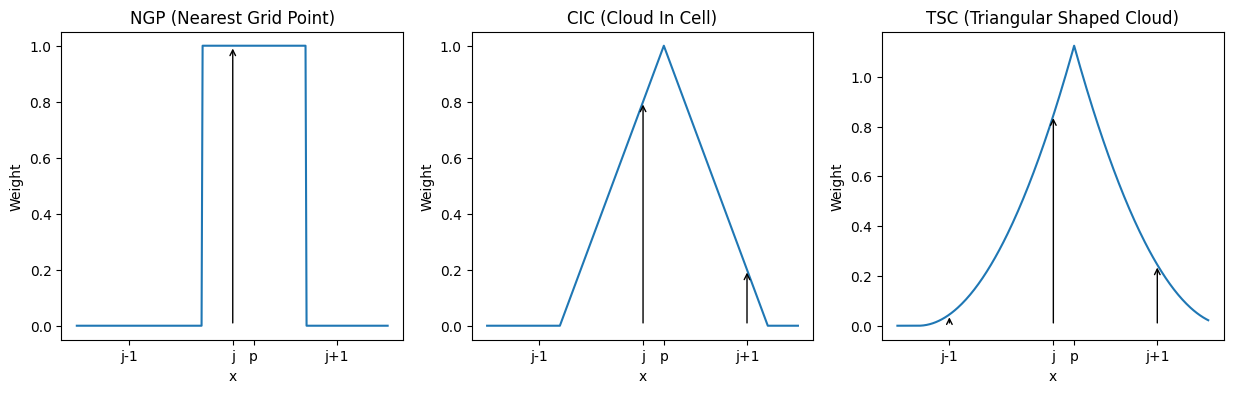
\includegraphics[width=\textwidth]{figures/weight_functions.png}
    \caption[Illustration of three mass assignment schemes]{Illustration of three mass assignment schemes—Nearest Grid Point (NGP), Cloud-In-Cell (CIC), and Triangular-Shaped Cloud (TSC)—used to map a particle's mass onto a 1D grid.}
    \label{fig:mass-assignment}
\end{figure}

\subsection{Parallelization Techniques}
Parallelization accelerates computations in large-scale simulations by leveraging multiple processors or computing nodes. Key strategies include:
\begin{itemize}
    \item \textbf{Domain Decomposition:} The computational domain is partitioned into smaller subdomains, each assigned to a separate processor \citep{1986Natur.324..446B}.
    \item \textbf{Task Parallelism:} Distributing independent tasks across multiple processors.
    \item \textbf{Data Parallelism:} Performing identical operations concurrently on different data elements, enabling SIMD (Single Instruction, Multiple Data) execution.
\end{itemize}

\subsection{Adaptive Mesh Refinement (AMR)}
Adaptive Mesh Refinement (AMR) dynamically adjusts grid resolution, refining the mesh where higher accuracy is needed (e.g., regions with high density gradients) and coarsening it elsewhere \citep{1989JCoPh..82...64B}. This technique is typically used in hydrodynamical simulations to capture complex fluid dynamics and shock fronts accurately.
Because N-body simulations with discrete particles do not require continuous field solution and have more efficient methods like Tree-PM, AMR is not commonly used in N-body simulations.

This creates a hierarchy of grids with increasing resolution and optimizes computational resources. Refinement is typically triggered when: 
\begin{equation}
    \left| \nabla \phi(\mathbf{x}) \right| > \theta,
\end{equation}
with $\theta$ being a predefined threshold.

\begin{figure}
    \centering
    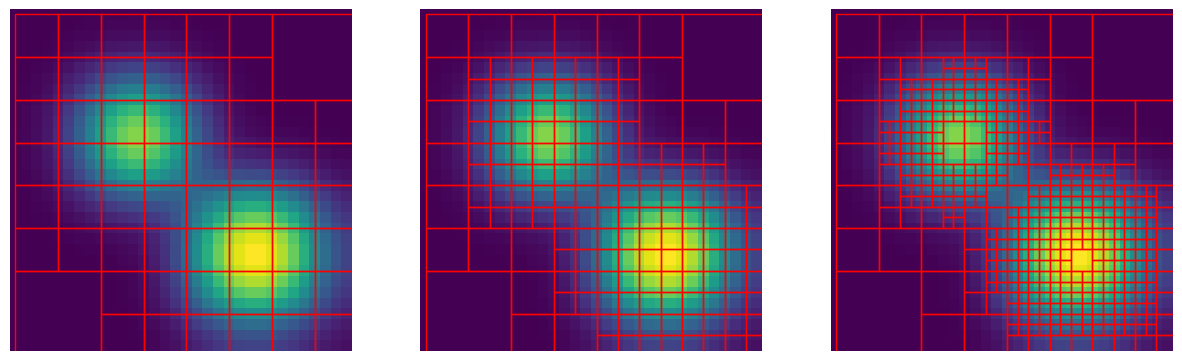
\includegraphics[width=\textwidth]{figures/adaptive_mesh_refinement.png}
    \caption[Illustration of adaptive mesh refinement]{Illustration of adaptive mesh refinement (AMR) applied to a 2D image with two Gaussian kernels. The left panel shows the initial coarse grid structure over the image. The middle and right panels demonstrate progressively finer levels of mesh refinement in regions of higher intensity, where the Gaussian kernels are located. The red grid outlines indicate the adaptively refined mesh hierarchy, ensuring higher resolution where needed while maintaining computational efficiency in lower-intensity regions.}
    \label{fig:amr}
\end{figure}
Figure~\ref{fig:amr} demonstrates the application of Adaptive Mesh Refinement (AMR) to a two-dimensional image containing two Gaussian kernels. Initially, a uniformly coarse grid overlays the entire image (left panel). As the refinement process progresses, the mesh becomes increasingly finer in regions with higher intensity, specifically around the Gaussian kernels (middle and right panels). The red grid lines represent the hierarchy of the refined meshes, enabling higher resolution where it is most needed and optimizing computational resources by keeping a coarser grid in less significant areas.

\subsection{Tree Construction}
Tree-based data structures efficiently organize hierarchical spatial data. The Barnes-Hut algorithm employs an octree to partition space, reducing computational complexity from $\mathcal{O}(N^2)$ to $\mathcal{O}(N \log N)$ by approximating distant particle clusters as single mass points. This approximation is controlled by the opening angle $\theta$:
\begin{equation}
    \frac{s}{d} < \theta,
\end{equation}
where $s$ is the node size and $d$ is the distance from the particle to the node's center of mass.

One of the popular algorithms for tree construction is the Barnes-Hut Octree \citep{1986Natur.324..446B}, which recursively subdivides the simulation volume into hierarchical grid cells. Figure~\ref{fig:barnes-hut} illustrates the Octree decomposition for a 3D volume containing four particles.
\begin{figure}[ht]
    \centering
    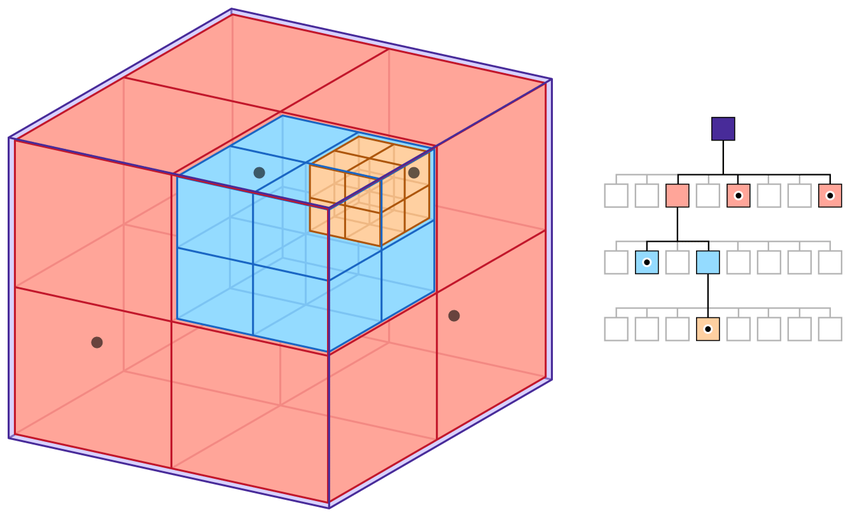
\includegraphics[width=0.6\textwidth]{figures/Octree.png}
    \caption[Illustration of an Octree decomposition]{Illustration of an Octree decomposition for a 3D volume containing four particles. The left panel showcases the spatial subdivision of the volume into hierarchical grid cells, with color-coding indicating different levels of refinement. The right panel presents the corresponding Octree data structure, highlighting the hierarchical relationships between nodes. Credit by \citet{Powell2023}}
    \label{fig:barnes-hut}
\end{figure}

Parallel tree construction involves building local trees within each subdomain and integrating them for global computations \citep{DUBINSKI1996133}. Efficient parallelization enhances scalability and performance in large-scale simulations.

\section{Advanced Codes and Methods: \texttt{FASTPM}} \label{sec:fastpm}
\texttt{FASTPM} (Fast Particle Mesh; \citealt{10.1093/mnras/stw2123}) is an advanced N-body simulation code tailored for efficiently modeling the evolution of dark matter and halo structures on cosmological scales. Building upon the foundational PM approach, \texttt{FASTPM} integrates modified kick and drift factors derived from the Zel'dovich Approximation (ZA). This enhancement allows \texttt{FASTPM} to achieve high accuracy in large-scale structure formation while significantly reducing computational overhead. This subsection delineates the core methodology of FASTPM, incorporating the mathematical formalism of its modified kick and drift factors.

\subsection{Modified Kick and Drift Factors}
The cornerstone of \texttt{FASTPM}'s enhanced performance lies in its \textbf{modified kick ($K_{\text{FASTPM}}$)} and \textbf{drift ($D_{\text{FASTPM}}$)} factors. These factors are meticulously derived from the Zel'dovich Approximation (ZA), a first-order Lagrangian perturbation theory (1LPT), to rectify inaccuracies in large-scale growth inherent in standard PM solvers, especially when operating with a limited number of time steps.

First, the Zel'dovich equation of motion to the first order is defined as:
\begin{eqnarray}
    \mathbf{x}_{\text{ZA}}(a) &=& \mathbf{q} + D(a)\mathbf{s}_1,  \nonumber \\
    \mathbf{p}_{\text{ZA}}(a) &=& a^3 E(a) g_p(a) \mathbf{s}_1,  \nonumber \\
    \mathbf{f}_{\text{ZA}}(a) &=& a^2 E(a) g_f(a) \mathbf{s}_1, 
\end{eqnarray}
where $E(a) = \frac{H(a)}{H(a=1)}$ is the dimensionless Hubble parameter, and $g_p(a)$ and $g_f(a)$ are auxiliary factors defined as:
\begin{eqnarray}
    g_p(a)  &=& \frac{dD}{da},  G_p(a) = D(a) \\[0.5em]
    g_f(a)  &=& \frac{d(a^3 E g_p)}{da}, G_f(a) = a^3 E g_p(a)
\end{eqnarray}
The ZA equations of motion are reformulated in terms of drift and kick operators by integrating over a time step from $a_0$ to $a_1$ and eliminating the ZA displacement $\mathbf{s}_1$:
\begin{eqnarray}
    \Delta \mathbf{x}_{\text{ZA}} &=& \mathbf{x}_{\text{ZA}}(a_1) - \mathbf{x}_{\text{ZA}}(a_0) \nonumber \\
    &=& \left[ D(a) \right]_{a_0}^{a_1} \mathbf{s}_1 \nonumber \\
    &=& \frac{\mathbf{p}_{\text{ZA}}(a_r)}{a_r^3 E(a_r)} \left( \frac{\Delta G_p}{g_p(a_r)} \right),
\end{eqnarray}
\begin{eqnarray}
    \Delta \mathbf{p}_{\text{ZA}} &=& \mathbf{p}_{\text{ZA}}(a_1) - \mathbf{p}_{\text{ZA}}(a_0) \nonumber \\
    &=& \frac{\mathbf{f}_{\text{ZA}}(a_r)}{a_r^2 E(a_r)} \left( \frac{\Delta G_f}{g_f(a_r)} \right),
\end{eqnarray}
where $\Delta \mathbf{x}_{\text{ZA}}$ is the change in displacement over the time step, $\Delta \mathbf{p}_{\text{ZA}}$ is the change in momentum over the time step, $a_r$ is a reference scale factor within the time step, $\Delta G_p = G_p(a_1) - G_p(a_0)$, and $\Delta G_f = G_f(a_1) - G_f(a_0)$.
Therefore, the modified kick and drift factors in FASTPM are defined as:
\begin{eqnarray}
    \mathcal{D}_{\text{FASTPM}} &=& \frac{\Delta \mathbf{x}_{\text{ZA}}}{\mathbf{p}_{\text{ZA}}} 
        = \frac{1}{a_r^3 E(a_r)} \left( \frac{\Delta G_p}{g_p(a_r)} \right) \\[1em]
    \mathcal{K}_{\text{FASTPM}} &=& \frac{\Delta \mathbf{p}_{\text{ZA}}}{\mathbf{f}_{\text{ZA}}} 
        = \frac{1}{a_r^2 E(a_r)} \left( \frac{\Delta G_f}{g_f(a_r)} \right) 
\end{eqnarray}
These operators ensure the exact integration of the ZA equations of motion, thereby accurately capturing the linear growth of structures within each time step.

\subsection{Algorithm Steps}
The main steps of the \texttt{FASTPM} algorithm follow the standard PM method discussed in Section~\ref{sec:pm-method}, with the addition of the modified kick and drift operators to ensure accurate linear growth.

\begin{enumerate}
    \item \textbf{Apply Modified Operators:}
    \label{fastpm:modified-kick-drift}
    Utilize the modified kick ($K_{\text{FASTPM}}$) and drift ($D_{\text{FASTPM}}$) factors to update particle velocities and positions. These factors, derived from the ZA, ensure accurate linear growth:
    
    \begin{enumerate}
        \item \textbf{Kick Step:}
        Update particle velocities by applying the gravitational acceleration scaled by the modified kick factor:
        \[
        \mathbf{v}_i\left(t + \frac{\Delta t}{2}\right) = \mathbf{v}_i(t) + \mathbf{g}_i(t) \cdot K_{\text{FASTPM}} \cdot \Delta t
        \]
        
        \item \textbf{Drift Step:}
        Update particle positions using the updated velocities and the modified drift factor:
        \[
        \mathbf{r}_i(t + \Delta t) = \mathbf{r}_i(t) + \mathbf{v}_i\left(t + \frac{\Delta t}{2}\right) \cdot D_{\text{FASTPM}} \cdot \Delta t
        \]
        
        \item \textbf{Second Kick Step:}
        Apply another kick to update velocities to the full time step:
        \[
        \mathbf{v}_i(t + \Delta t) = \mathbf{v}_i\left(t + \frac{\Delta t}{2}\right) + \mathbf{g}_i(t + \Delta t) \cdot K_{\text{FASTPM}} \cdot \Delta t
        \]
    \end{enumerate}
    
    \item \textbf{Update Particle States:}
    Finalize the update of particle velocities and positions after applying the modified kick and drift operators:
    \[
    \mathbf{v}_i(t + \Delta t) = \mathbf{v}_i\left(t + \frac{\Delta t}{2}\right) + \mathbf{g}_i(t + \Delta t) \cdot K_{\text{FASTPM}} \cdot \Delta t
    \]
    \[
    \mathbf{r}_i(t + \Delta t) = \mathbf{r}_i(t) + \mathbf{v}_i\left(t + \frac{\Delta t}{2}\right) \cdot D_{\text{FASTPM}} \cdot \Delta t
    \]
    
    \item \textbf{Advance Time:}
    Increment the simulation time by the time step $\Delta t$:
    \[
    t \leftarrow t + \Delta t
    \]
\end{enumerate}

\section{Generating Weak Lensing Maps from Simulations}
\label{sec:weak-lensing-generation}
To extract statistics from N-body simulations, it is necessary to generate detailed WL maps by simulating the propagation of a vast number of virtual light rays from source galaxies to the observer. This process involves calculating the distortions and magnifications of the source images caused by the cumulative gravitational deflections from the intervening matter distribution along each line of sight.

\subsection{Conventional Ray-Tracing Algorithm}
\label{subsec:conventional-ray-tracing}
Conventional ray-tracing algorithms are fundamental tools for generating WL maps from N-body simulations. These algorithms simplify the complex three-dimensional matter distribution by projecting it onto a series of two-dimensional lens planes. The numerical implementation of the ray-tracing algorithm involves several key computational steps, outlined below \citep{2008ApJ...682....1D, 2009A&A...497..335T, 2015MNRAS.453.3043S}:

\begin{enumerate}
    \item \textbf{Lens Plane Generation:} 
    The first step involves constructing the surface mass density $\Delta_\Sigma^j(\boldsymbol{\theta})$ for each lens plane $j$. This is achieved by projecting the three-dimensional matter density $\rho(\chi, \chi\boldsymbol{\theta})$ within a spherical shell bounded by comoving distances $\chi_j$ and $\chi_{j+1}$ onto a two-dimensional plane:
    \begin{equation}
        \Delta_\Sigma^j(\boldsymbol{\theta}) = \int_{\chi_j}^{\chi_{j+1}} \left[ \rho(\chi, \chi\boldsymbol{\theta}) - \bar{\rho}(\chi) \right] \chi^2 \, \mathrm{d}\chi,
    \end{equation}
    where $\bar{\rho}(\chi)$ is the mean matter density at distance $\chi$. 
    The effective comoving distance to the center of the $j$-th shell, $\chi^j$, is calculated as \citep{2015MNRAS.453.3043S}:
    \begin{equation}
        \chi^j = \frac{\int_{\chi_{\min}}^{\chi_{\max}} \chi^3 \, \mathrm{d}\chi}{\int_{\chi_{\min}}^{\chi_{\max}} \chi^2 \, \mathrm{d}\chi} = \frac{3}{4} \frac{\chi_{\max}^4 - \chi_{\min}^4}{\chi_{\max}^3 - \chi_{\min}^3},
    \end{equation}
    where $\chi_{\min}$ and $\chi_{\max}$ are the minimum and maximum comoving distances of the shell, respectively.
    The convergence field $\kappa_j(\boldsymbol{\theta})$ for the $j$-th lens plane is then computed as:
    \begin{equation}
        \kappa_j(\boldsymbol{\theta}) = \frac{4\pi G}{c^2} \frac{\Delta_\Sigma^j(\boldsymbol{\theta})}{a_j \chi_j},
    \end{equation}
    with $a_j$ being the scale factor and $\chi_j$ the comoving distance to the $j$-th lens plane.

    To express $\kappa_j(\boldsymbol{\theta})$ in terms of the simulation parameters, we consider the following quantities:
    \begin{itemize}
        \item $V_{\mathrm{sim}}$: The simulation volume.
        \item $N_{\mathrm{part}}$: The total number of particles in the simulation.
        \item $N_{\mathrm{pix}}$: The number of pixels on each lens plane.
        \item $n_{\mathrm{part}}^j$: The number of particles in the $j$-th shell.
        \item $\bar{n}_{\mathrm{part}}^j$: The mean number of particles per pixel in the $j$-th shell.
    \end{itemize}
    The convergence field is then given by:
    \begin{equation}
        \kappa_j(\boldsymbol{\theta}) = \frac{3H_0^2\Omega_m}{2c^2 a_j \chi_j} \frac{V_{\mathrm{sim}}}{N_{\mathrm{part}}} \frac{N_{\mathrm{pix}}}{4\pi} \left( n_{\mathrm{part}}^j - \bar{n}_{\mathrm{part}}^j \right),
    \end{equation}

    \item \textbf{Potential Calculation:} 
    To facilitate the computation of lensing effects, the lensing potential $\psi^j(\boldsymbol{\theta})$ for each lens plane is derived from the convergence field $\kappa_j(\boldsymbol{\theta})$. This is efficiently done using spherical harmonics:
    \begin{equation}
        \psi_{lm}^j = \frac{2}{l(l+1)} \kappa_{lm}^j \quad \text{for} \quad l \neq 0,
    \end{equation}
    and $\psi_{lm}^j = 0$ for $l = 0$. Subsequently, the lensing potential in real space is reconstructed, allowing the calculation of the deflection field $\boldsymbol{\alpha}^j(\boldsymbol{\theta})$ and the optical tidal matrix $U_{ik}^j(\boldsymbol{\theta})$ through:
    \begin{equation}
        \alpha_i^j = -\nabla_i \psi^j, \quad U_{ik}^j = \nabla_i \nabla_k \psi^j.
    \end{equation}

    \item \textbf{Deflection Angle Determination:} 
        The deflection field $\boldsymbol{\alpha}^j(\boldsymbol{\theta})$ and the optical tidal matrix $U_{ik}^j(\boldsymbol{\theta})$ are interpolated to arbitrary positions on each lens plane. The lensing matrix $\mathcal{A}^j_{ik}$ at each plane is then updated using the recurrence relation:
        \begin{equation}
            \begin{aligned}
                \mathcal{A}_{i k}^{j+1} & = \left(1 - \frac{\chi_j}{\chi_{j+1}} \frac{\chi_{j+1} - \chi_{j-1}}{\chi_j - \chi_{j-1}} \right) \mathcal{A}_{i k}^{j-1} + \frac{\chi_j}{\chi_{j+1}} \frac{\chi_{j+1} - \chi_{j-1}}{\chi_j - \chi_{j-1}} \mathcal{A}_{i k}^j \\
                & \quad - \frac{\chi_{j+1} - \chi_j}{\chi_{j-1}} U_{i m}^j \mathcal{A}_{m k}^j,
            \end{aligned}
        \end{equation}
        with the initial conditions:
        \begin{equation}
            \mathcal{A}_{i k}^1 = \delta_{i k}, \quad \mathcal{A}_{i k}^0 = \delta_{i k},
        \end{equation}
    for $j \geq 1$. The closest lens plane to the observer is designated as $j = 0$.

    \item \textbf{Ray Propagation:} 
    Light rays are propagated from the source galaxies to the observer through the sequence of lens planes. At each plane, the accumulated deflection angles are updated based on the lensing matrix $\mathcal{A}^j_{ik}$. 

    \item \textbf{Map Assembly:} 
    After propagating all light rays through the lens planes, the convergence $\kappa(\boldsymbol{\theta})$ and shear $\gamma(\boldsymbol{\theta})$ fields are compiled into full-sky maps, using Eq.~\eqref{eq:jacobian_matrix}. These maps are typically represented on the \texttt{HEALPix} grid.
\end{enumerate}

\subsection{Born-approximated Ray-tracing}
The Born approximation offers a simplified approach to weak lensing map generation by assuming that light rays travel along their unperturbed, straight-line paths from the source galaxies to the observer. This approximation neglects the bending of light rays due to gravitational deflections between lens planes, thereby reducing the computational complexity of the ray-tracing process \citep{2006glsw.conf..269S}. 

While this simplification can lead to faster computations, it introduces certain limitations in accurately capturing multiple deflections and non-linear lensing effects. 
To overcome these limitations, researchers have developed Post-Born corrections \citep{2002ApJ...574...19C, 2005PhRvD..72j3004D} that account for the deflection during ray propagation and for the so-called lens-lens coupling, which describes how gravitational lenses at different redshifts can interact to generate rotational modes in the observable fields. It is shown that the Post-Born corrections can impact the higher-order moments or peak statistics of galxy weak lensing convergence maps \citep{2017PhRvD..95l3503P, 2019JCAP...10..057F}. Figure~\ref{fig:born-approximation} \citep{2017PhRvD..95l3503P} illustrates the parameter bias induced by the Born approximation in the convergence power spectrum and moments of the convergence field. The Born approximation is accurate in predicting the convergence power spectrum, but it leads to significant biases in the moments of the convergence field.

\begin{figure}[ht]
    \centering
    \begin{subfigure}[b]{0.48\textwidth}
        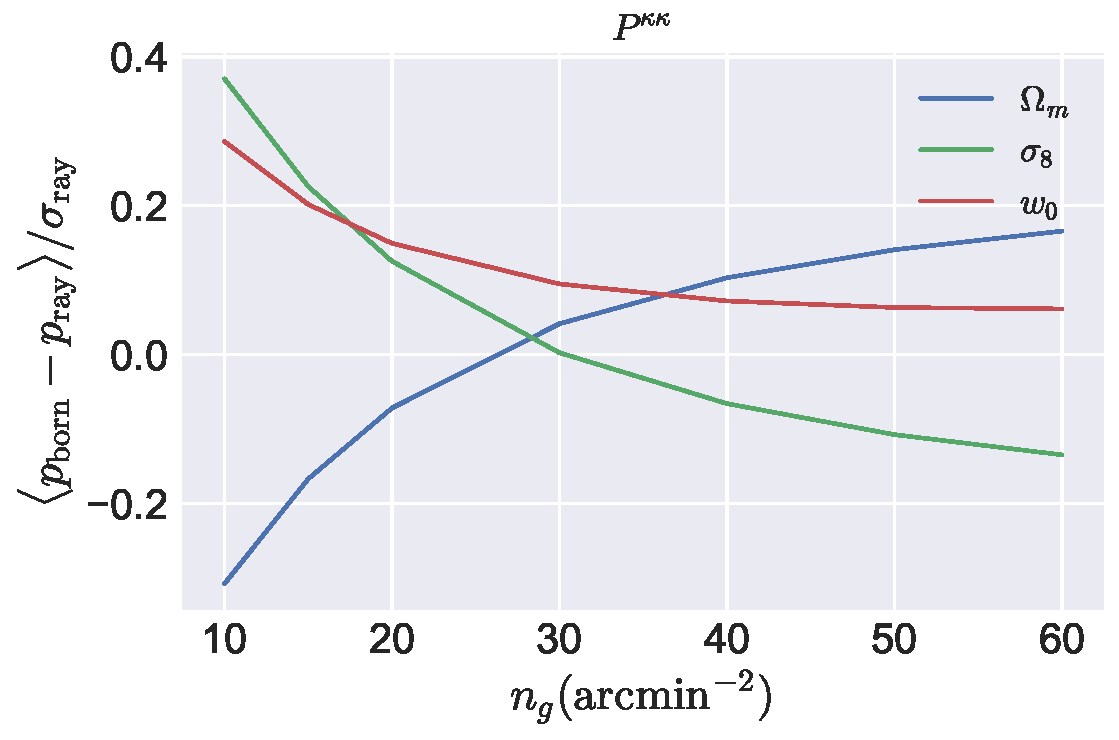
\includegraphics[width=\textwidth]{figures/bias_ngal_convergence_powerSN_s0_nb100.pdf}
    \end{subfigure}
    \hfill
    \begin{subfigure}[b]{0.48\textwidth}
        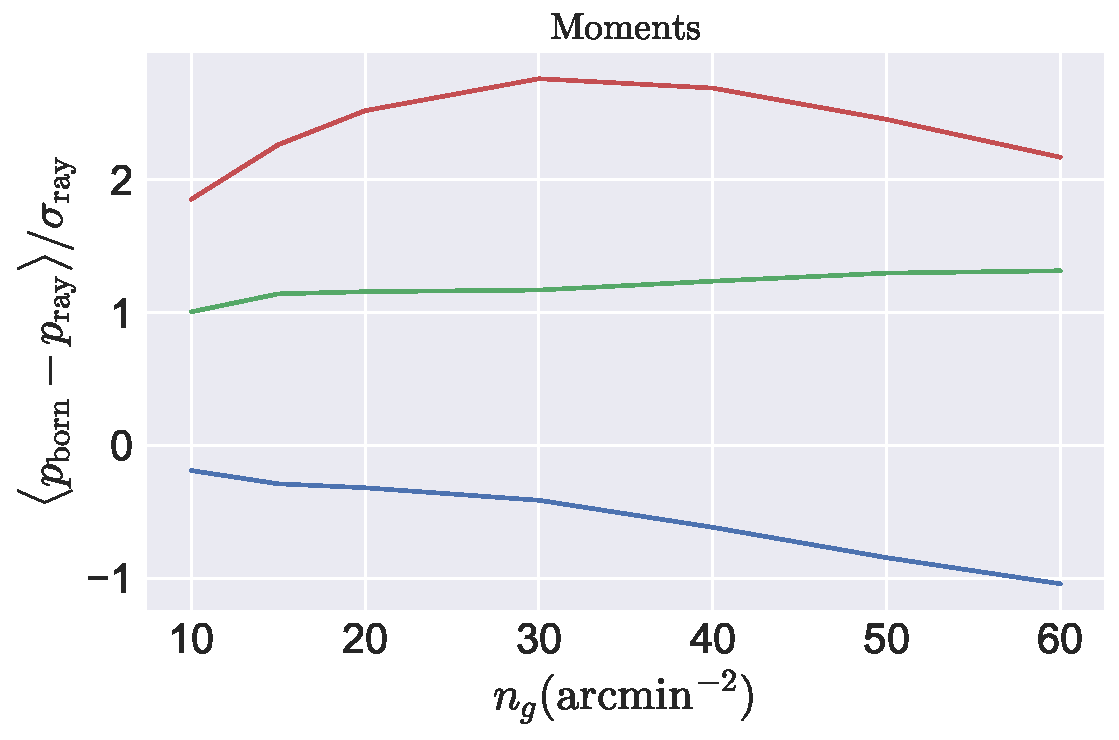
\includegraphics[width=\textwidth]{figures/bias_ngal_convergence_momentsSN_s50_nb9.pdf}
    \end{subfigure}
    \caption[Parameter bias induced by the Born approximation]{Parameter bias induced by the Born approximation in the convergence power spectrum (Left Panel) and moments of the convergence field (Right Panel). While the Born approximation is accurate in predicting the convergence power spectrum, it leads to significant biases in the moments of the convergence field. credit by \citet{2017PhRvD..95l3503P}}
    \label{fig:born-approximation}
\end{figure}

Nonetheless, the Born-approximation remains a valuable tool for generating weak lensing maps in large-scale structure studies \citep{2008MNRAS.391..435F, 2009A&A...499...31H, 2015MNRAS.447.1319F}.
The Born-approximated ray-tracing algorithm comprises the following key steps:

\begin{enumerate}
    \item \textbf{Lens Plane Calculation:} 
    For each lens plane $j$, the convergence contribution $\kappa_j(\boldsymbol{\theta})$ is computed independently, incorporating the lensing efficiency function $W(\chi_j, \chi_s)$, where $\chi_j$ is the comoving distance to the $j$-th lens plane and $\chi_s$ is the comoving distance to the source galaxy. The convergence on the $j$-th plane is given by
    \begin{equation}
        \kappa_j(\boldsymbol{\theta}) = W(\chi_j, \chi_s) \delta_j(\boldsymbol{\theta}) \Delta \chi_j,
        \label{eq:kappa_born}
    \end{equation}
    where $\delta_j(\boldsymbol{\theta}) = n_{\mathrm{part}}^j(\boldsymbol{\theta}) / \bar{n}_{\mathrm{part}}^j - 1$ represents the projected matter density contrast on the $j$-th lens plane, and $\Delta \chi_j$ is the comoving thickness of the $j$-th lens plane. The lensing efficiency function, previously defined in Eq.~\eqref{eq:lensing_efficiency_flat}, is discreditized for each lens plane as:
    \begin{equation}
        W(\chi_j, \chi_s) = \frac{3 H_0^2 \Omega_m}{2 c^2} \frac{( \chi_s - \chi_j )}{ \chi_s } \frac{ \chi_j }{ a_j },
    \end{equation}

    \item \textbf{Convergence Field Assembly:} 
    The total convergence field $\kappa(\boldsymbol{\theta})$ is obtained by summing the contributions from all individual lens planes:
    \begin{equation}
        \kappa(\boldsymbol{\theta}) = \sum_{j} \kappa_j(\boldsymbol{\theta}).
        \label{eq:total_kappa}
    \end{equation}
    This linear superposition is a direct consequence of the Born approximation, which assumes that each lens plane contributes independently to the total convergence without accounting for the altered path of the light ray due to previous deflections.

\end{enumerate}


\chapter{Methods}
\section{Dataset Overview}
To achieve high accuracy while minimizing computational time, we employed the \texttt{FASTPM} particle-mesh simulation code \citep{10.1093/mnras/stw2123}. This code enhances convergence by adjusting kick and drift factors to closely adhere to the Zel'dovich approximation, thereby improving the efficiency of structure formation modeling.

In our study, we quantify super-sample covariance in higher-order statistics using two N-body simulations: \textbf{BIGBOX} and \textbf{TILED}. The \textbf{BIGBOX} simulation, conducted as part of the HalfDome project \citep{2024arXiv240717462B}, encompasses a large cosmic volume, whereas the \textbf{TILED} simulation represents a smaller volume with the same resolution as BIGBOX, specifically excluding large-scale modes. The cosmological parameters for both simulations align with those of IllustrisTNG \citep{2019ComAC...6....2N}, as listed in Table~\ref{tab:simulations}.

\begin{table}[h]
\centering
\begin{tabular}{lcc}
\toprule
\textbf{Parameter} & \textbf{Symbol} & \textbf{Value} \\
\midrule
Hubble constant & $H_0$ & 67.74 \, [$\mathrm{km\,s^{-1}\,Mpc^{-1}}$] \\ 
Matter density & $\Omega_m$ & 0.3089 \\
Baryon density & $\Omega_b$ & 0.0486 \\
Amplitude of fluctuations & $\sigma_8$ & 0.8159 \\
Spectral index & $n_s$ & 0.9667 \\
Sum of neutrino masses & $M_{\nu}$ & 0.0 \, [eV] \\
\bottomrule
\end{tabular}
\caption{Cosmological parameters used in the N-body simulations.}\label{tab:simulations}
\end{table}

The \textbf{BIGBOX} simulation models an extensive cubic volume of $L = 3750$ Mpc/h with $6144^3$ particles, enabling detailed capture of large-scale structures. From this data, a full-sky map was generated by first covering an octant of the sky and subsequently extending it to a full-sky projection.

The \textbf{TILED} simulation covers a smaller volume of $L = 625$ Mpc/h, populated with $1024^3$ particles. To achieve resolution parity with the BIGBOX simulation, multiple smaller volumes were tiled together, forming a full-sky map comparable in detail to the BIGBOX simulation but without the inclusion of large-scale modes.

Both simulations commence at an initial redshift of $z = 9$, utilizing an initial linear matter power spectrum at $z = 0$ generated via the \texttt{CLASS} code \citep{2011JCAP...07..034B}. This setup ensures consistency with observational data of the early universe. We evolved the simulations over 60 time steps, reaching the present day ($z = 0$), thereby capturing the non-linear growth of cosmic structures—an aspect crucial for studies of weak gravitational lensing.

\begin{figure}[ht]
    \centering
    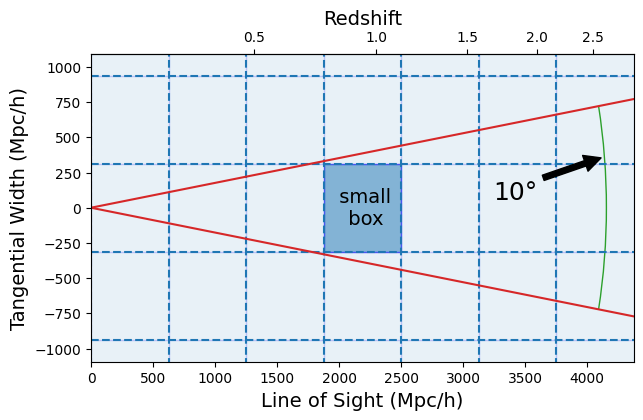
\includegraphics[width=0.8\textwidth]{figures/light_cone_configuration.png}
    \caption{Spatial and redshift setup for the \textbf{BIGBOX} and \textbf{TILED} simulations. The left side of the figure features red lines delineating the light cone boundaries, covering a $10^\circ$ field of view on the sky. Overlaid on this are dashed blue grids that partition the overall simulation volume into smaller, manageable tiling regions. Within these grids, the "small box" highlights a specific tiled region that resides inside the extensive BIGBOX volume. The horizontal axis represents the line-of-sight distance measured in comoving megaparsecs per $h$, with the corresponding redshift values displayed on the top axis.} \label{fig:simulationsetting}
\end{figure}
Figure~\ref{fig:simulationsetting} showcases the spatial and redshift setup for the \textbf{BIGBOX} and \textbf{TILED} simulations used in cosmological studies. The left side of the figure features red lines delineating the light cone boundaries, covering a $10^\circ$ field of view on the sky. Overlaid on this are dashed blue grids that partition the overall simulation volume into smaller, manageable tiling regions. Within these grids, the "small box" highlights a specific tiled region that resides inside the extensive BIGBOX volume. The horizontal axis represents the line-of-sight distance measured in comoving megaparsecs per $h$, with the corresponding redshift values displayed on the top axis. 

\section{Generating Convergence Maps}
To simulate the weak gravitational lensing effect observed in surveys, we generated convergence maps from our N-body simulations. Light cones were constructed from these simulations to model the observable universe, with particles inserted on-the-fly at the appropriate redshifts through interpolation between N-body time steps.

To balance computational efficiency with the need to accurately capture lensing effects, we set the width of each radial shell to $\Delta a = 0.01$, corresponding to a comoving distance of approximately $\Delta \chi \approx 100 \, h^{-1} \, \text{Mpc}$.

For each shell, the three-dimensional matter density $\delta(\mathbf{x}, z_i)$ was projected onto a two-dimensional plane perpendicular to the line of sight. The projected surface density $\Sigma(\hat{\mathbf{n}}, \chi_i)$ at an angular position $\hat{\mathbf{n}}$ was computed by integrating the matter density within the shell along the radial direction:
\begin{equation}
    \Sigma(\hat{\mathbf{n}}, \chi_i) = \int_{\chi_i}^{\chi_{i+1}} \delta(\chi \hat{\mathbf{n}}, z(\chi)) \, d\chi.
\end{equation}
In practice, the surface density was mapped onto a HEALPix grid \citep{Górski_2005} to create a full-sky map $\Sigma(n_j, \chi_i)$, where $n_j$ represents discretized angular positions. The HEALPix grid resolution was set to $N_{\text{side}} = 8192$, providing an angular resolution of approximately $0.43$ arcminutes, which is sufficient to capture small-scale structures relevant to weak lensing studies.

The convergence $\kappa(n_j; z_s)$ at each pixel of the HEALPix grid was then obtained by summing contributions from all the shells up to the source redshift:
\begin{equation}
    \kappa(n_j; z_s) = \sum_{i} W(\chi_i, \chi_s) \Sigma(n_j, \chi_i) \Delta \chi_i,
\end{equation}
where $W(\chi, \chi_s)$ is the lensing efficiency function.
The effective comoving distance to the center of the $j$-th shell, $\chi^j$, is calculated as \citep{2015MNRAS.453.3043S}:
\begin{equation}
    \chi^j = \frac{\int_{\chi_{\min}}^{\chi_{\max}} \chi^3 \, \mathrm{d}\chi}{\int_{\chi_{\min}}^{\chi_{\max}} \chi^2 \, \mathrm{d}\chi} = \frac{3}{4} \frac{\chi_{\max}^4 - \chi_{\min}^4}{\chi_{\max}^3 - \chi_{\min}^3},
\end{equation}
The density contrast within the $i$-th pixel of the $j$-th shell, $\delta^j(\hat{\boldsymbol{n}}_i)$, is determined by:
\begin{equation}
    \delta^j(\hat{\boldsymbol{n}}_i) = \frac{n_{\mathrm{part}, i}^j}{\bar{n}_{\mathrm{part}}^j} - 1,
\end{equation}
where $n_{\mathrm{part}, i}^j$ is the number of particles in the $i$-th pixel of the $j$-th shell, and $\bar{n}_{\mathrm{part}}^j$ is the average number of particles per pixel in that shell.

We considered source redshifts $z_s$ from 0.5 to 2.5 in increments of 0.5, covering the range of distances relevant for current and future galaxy surveys, such as DES, LSST, \textit{Euclid}, and \textit{Roman}.

\begin{figure}
    \centering
    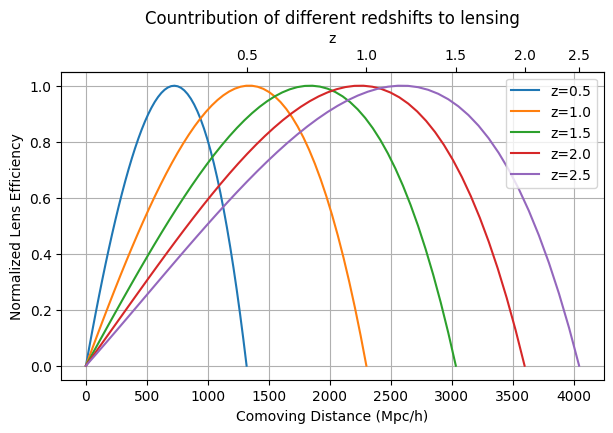
\includegraphics[width=0.8\textwidth]{figures/lensefficiency.png}
    \caption{Normalized lensing efficiency as a function of comoving distance for multiple source redshifts. The lensing efficiency peaks at intermediate comoving distances, indicating regions where the distribution of matter enhances the gravitational lensing signal.} \label{fig:lensing_efficiency}
\end{figure}
Figure~\ref{fig:lensing_efficiency} presents the normalized lensing efficiency as a function of comoving distance (measured in Mpc/$h$) for multiple source redshifts ($z$). Each curve corresponds to a specific source redshift, as detailed in the legend. The lensing efficiency curves exhibit peaks at intermediate comoving distances, indicating the regions where the distribution of matter along the line of sight most significantly enhances the gravitational lensing signal. 

\section{Incorporating Noise}
In real observations, measurements of the lensing signal are contaminated by noise arising from the intrinsic shapes of galaxies and errors in shape measurements. This noise, referred to as shape noise, constitutes a significant source of uncertainty, particularly on small angular scales.

To simulate shape noise, we added Gaussian noise to our convergence maps. We considered four different surveys with varying galaxy number densities, as detailed in Table~\ref{tab:noise}.

\begin{table}[h]
\centering
\begin{tabular}{lc}
\toprule
\textbf{Survey} & \textbf{Galaxy Number Density} [$\mathrm{arcmin}^{-2}$] \\
\midrule
DES/KiDS & 7 \\
HSC & 15 \\
\textit{Euclid}/LSST & 30 \\
\textit{Roman} & 50 \\
\bottomrule
\end{tabular}
\caption{Galaxy number densities for different surveys used to model shape noise levels.}\label{tab:noise}
\end{table}

The variance of the shape noise per pixel was calculated as:
\begin{equation}
    \sigma_{\kappa, \text{noise}}^2 = \frac{\sigma_{\epsilon}^2}{2 n_{\mathrm{gal}} A_{\mathrm{pix}}},
\end{equation}
where $\sigma_{\epsilon}$ is the intrinsic ellipticity dispersion of galaxies, set to $\sigma_{\epsilon} = 0.26$ \citep{2019A&A...627A..59E}, $n_{\mathrm{gal}}$ is the galaxy number density per square arcminute, and $A_{\mathrm{pix}}$ is the solid angle of a pixel, set to $0.43$ arcminutes$^2$.
We generated a Gaussian random field $n(\hat{\mathbf{n}})$ with the calculated variance and added it to the convergence maps:
\begin{equation}
    \kappa_{\mathrm{obs}}(\hat{\mathbf{n}}) = \kappa(\hat{\mathbf{n}}) + n(\hat{\mathbf{n}}).
\end{equation}

\section{Patch Extraction for Analysis}
In order to simlplify the analysis onto a flat patch, we extracted patches from the full-sky convergence maps. Each patch covers an area of $10^\circ \times 10^\circ$ and is uniformly distributed across the sky using a Fibonacci grid \citep{2006QJRMS.132.1769S, 2023MNRAS.524.5591F}. The center of each patch is positioned at the vertices of the Fibonacci grid defined by golden ratio spirals:
\begin{equation}
    \sin \theta_i = \frac{2i}{2N + 1}, \quad \phi_i = \frac{2 \pi i}{\varphi}, \quad -N \leq i \leq N, \quad -\frac{\pi}{2} \leq \theta_i \leq \frac{\pi}{2},
\end{equation}
where $N$ is the number of patches and $\varphi = (1 + \sqrt{5})/2$ is the golden ratio.

The number of patches, denoted \( N_{\text{patches}} \), was optimized to ensure that individual patches do not overlap, except in regions near the poles where overlapping patches were subsequently discarded. The optimization process commenced with an initial count of \( N_{\text{patches}} = 400 \) and involved iteratively reducing this number until a configuration was achieved wherein the patches remained non-overlapping, except for centers located within \( 10\sqrt{2}^\circ \, \mathrm{\deg}\) of the poles, that is $|\theta_i| \geq 10\sqrt{2}^\circ$ and $|\phi_i| \leq \pi - 10\sqrt{2}^\circ$. Additionally, patches include points heavily tiled along with line of sight and near the equator are excluded to avoid severe Box Replication Effect (see Sec.~\ref{sec:boxreplication} for further check).
After optimization and masking, the number of patches was set to $N_{\text{patches}} = 273$, effectively reducing to $N_{\text{patches}} = 262$, effectively cover $64 \%$ of the sky. The visualization of the Fibonacci grid is shown in Figure~\ref{fig:fibonacci}.
\begin{figure}[ht]
    \centering
    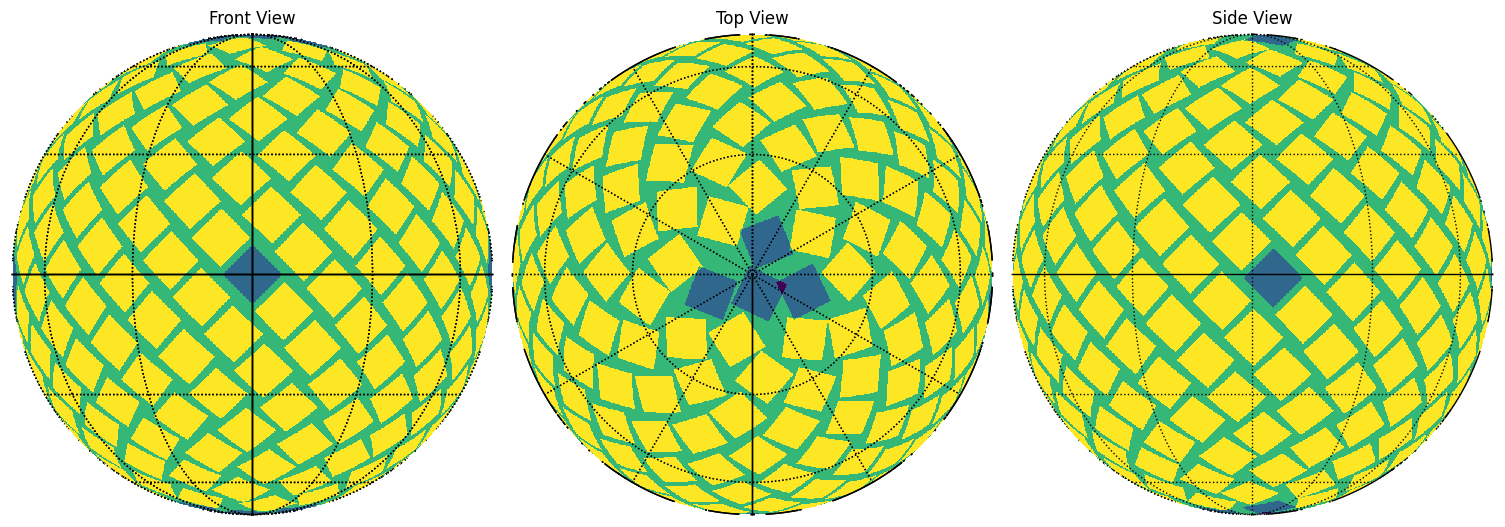
\includegraphics[width=0.8\textwidth]{figures/fibonacci_grid.png}
    \caption{Visualization of the Fibonacci grid with $N_{\text{patches}} = 273$ patches, each covering approximately $10 \times 10$\,deg$^2$. 
    After the optimization and masking, the number of patches is reduced to $N_{\text{patches}} = 262$, effectively covering $64 \%$ of the sky.
    Each panel show the patches distribution on the Front, Top and Side view.}\label{fig:fibonacci}
\end{figure}

To verify the absence of overlap between patches, we calculated the vertices of each patch and conducted pairwise overlap checks with all other patches. For a Fibonacci grid center characterized by coordinates \( (\theta_i, \phi_i) \), the vertices of the corresponding patch are defined as:
\begin{align}
    \left( \theta_i - \Delta \theta,\, \phi_i - \Delta \phi \right), \quad &\left( \theta_i - \Delta \theta,\, \phi_i + \Delta \phi \right), \nonumber \\
    \left( \theta_i + \Delta \theta,\, \phi_i - \Delta \phi \right), \quad &\left( \theta_i + \Delta \theta,\, \phi_i + \Delta \phi \right),
\end{align}
where
\begin{align}
    \Delta \theta = 5\sqrt{2}\, \mathrm{\deg}, \quad \Delta \phi = 5\sqrt{2}\sin \theta_i \, \mathrm{\deg}.
\end{align}

Using the vertices of the Fibonacci grid as centers, we employed the \texttt{gnomview} function from the \texttt{healpy} library \citep{Zonca2019} to project each spherical patch onto a flat plane via a gnomonic projection. Each patch is represented by a $2048 \times 2048$ grid of pixels, resulting in a pixel size of:
\begin{equation}
    \Delta \theta = \frac{10^\circ}{2048} \approx 0.00488^\circ \approx 0.293' \quad \text{per pixel}.
\end{equation}

\section{Gaussian Smoothing}
Shape noise predominantly affects small angular scales. To mitigate this noise and enhance the detection of the underlying lensing signal, we applied Gaussian smoothing to the noisy convergence maps. The Gaussian filter used is defined by:
\begin{equation}
    W(\theta) = \frac{1}{\pi \theta_{\mathrm{G}}^2} \exp\left( -\frac{\theta^2}{\theta_{\mathrm{G}}^2} \right),
\end{equation}
where $\theta$ is the angular distance from the center of the filter, and $\theta_{\mathrm{G}}$ is the smoothing scale. For our analysis, we selected $\theta_{\mathrm{G}} = 2'$, $5'$, $8'$, and $10'$.

By convolving the noisy convergence map with the Gaussian filter, we obtained the smoothed convergence map:
\begin{equation}
    \kappa_{\mathrm{smoothed}}(\hat{\mathbf{n}}) = \int d\Omega' \, W(|\hat{\mathbf{n}} - \hat{\mathbf{n}}'|) \kappa_{\mathrm{obs}}(\hat{\mathbf{n}}').
\end{equation}

Figure~\ref{fig:smoothing} demonstrates the application of Gaussian smoothing to a noisy convergence map. The figure presents four panels, each corresponding to a different smoothing scale: $\theta_{\mathrm{G}} = 2'$, $5'$, $8'$, and $10'$. As the smoothing scale increases, the convolution of the convergence map with the Gaussian filter effectively reduces small-scale noise, as evidenced by the diminishing high-frequency fluctuations in the map. 
\begin{figure}[ht]
    \centering
    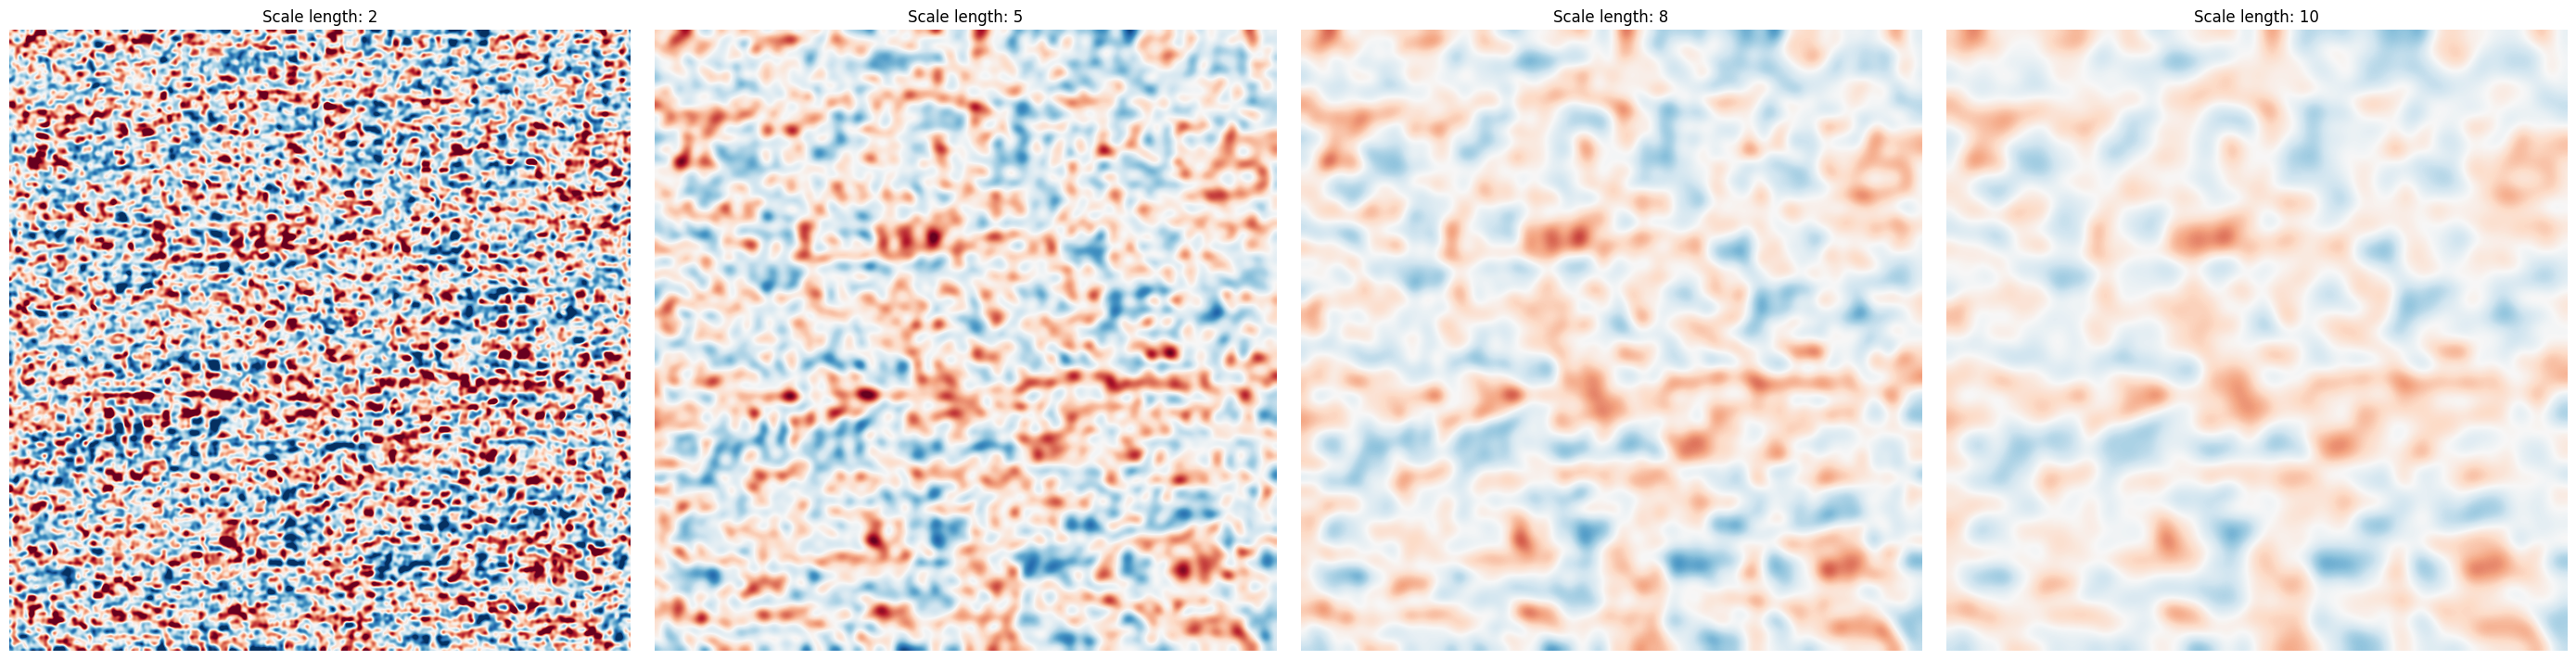
\includegraphics[width=\textwidth]{figures/smoothed_comparison.png}
    \caption{Effect of Gaussian smoothing on a noisy convergence map. Each panel shows the result of applying a Gaussian filter with a different smoothing scale $\theta_{\mathrm{G}} = 2'$, $5'$, $8'$, and $10'$. As the smoothing scale increases, small-scale noise is progressively suppressed, and large-scale structures become more prominent. This demonstrates how Gaussian smoothing effectively reduces shape noise while enhancing the detection of the underlying lensing signal.}
\label{fig:smoothing}
\end{figure}

\section{Measurements}
In order to characterize the influence of super-sample covariance on higher-order statistics, this study concentrates on the bispectrum, probability distribution function (PDF), peak counts, minima counts, and Minkowski functionals. These statistical measures offer complementary insights into the underlying matter distribution and exhibit sensitivity to distinct features of the gravitational lensing signal.

\subsection{Statistical Measures and Computational Methods}
Table~\ref{tab:statistics} delineates the range of values and the computational subroutines employed for each statistical measure. Each statistic is computed both for full-sky analyses and sky patches, utilizing the appropriate methodologies as specified.
\begin{table*}[htbp]
    \centering
    \begin{tabular}{lcc}
    \toprule
    \textbf{Statistic} & \textbf{Range} & \textbf{Subroutine (Sky Patch)} \\
    \midrule
    Angular Power Spectrum & $300 \leq \ell \leq 3000$ & \texttt{lenstools.powerSpectrum} \\
    Bispectrum & $300 \leq \ell \leq 3000$ & \texttt{lenstools.bispectrum} \\
    Peak Counts & $-4 \leq \kappa/\sigma_\kappa \leq 4$ & \texttt{lenstools.peakCount} \\
    Minima Counts & $-4 \leq \kappa/\sigma_\kappa \leq 4$ & \texttt{lenstools.peakCount} \\
    Probability Distribution Function (PDF) & $-4 \leq \kappa/\sigma_\kappa \leq 4$ & \texttt{lenstools.pdf} \\
    Minkowski Functionals & $-4 \leq \kappa/\sigma_\kappa \leq 4$ & \texttt{lenstools.minkowskiFunctionals} \\
    \bottomrule
    \end{tabular}
    \caption{Summary of the statistical measures employed in this investigation, including their respective value ranges and computational subroutines utilized for both full-sky and sky-patch analyses.}\label{tab:statistics}
\end{table*}
The angular power spectrum, denoted as $C_{\ell}^{\kappa\kappa}$, alongside three configurations of the bispectrum, $B_{\ell_1\ell_2\ell_3}^{\kappa\kappa\kappa}$, are derived from unsmoothed convergence maps. The bispectrum calculations encompass three distinct configurations: equilateral ($\ell_1 = \ell_2 = \ell_3$), squeezed ($\ell_1 = \ell_2 = 10\ell_3$), and isosceles ($\ell_1 = \ell_2 = 2\ell_3$). 
All bispectrum and angular power spectrum computations are confined within the multipole range $\ell \in [300, 3000]$, consistent with the multipole selection in the HSC Y3 cosmic shear analysis \citep{2023PhRvD.108l3519D}. We adopt a logarithmic binning approach to effectively sample the range of scales, dividing the multipole interval into 8 bins that are evenly spaced in logarithmic space. 

Conversely, the PDF, peak counts, minima counts, and Minkowski functionals are derived from smoothed convergence maps, where the smoothing angle is fixed at 2 arcminutes for the primary results. These measurements are conducted within the normalized range $-4 \leq \kappa/\sigma_{\kappa} \leq 4$, linearly divided into 8 bins following \citet{2021A&A...648A.115M}. $\sigma_{\kappa}$ denotes the standard deviation of each patch's convergence map.

All statistical computations are performed using the \texttt{lenstools} package \citep{2016A&C....17...73P}.

\subsection{Covariance Matrix Estimation}
Following the measurement phase, this study examines the influence of super-sample covariance on the covariance matrices associated with the aforementioned statistical measures. To achieve this, we employ an unbiased estimator for the covariance matrix as previously defined in Equation~\ref{eq:covariance}. The analysis utilizes 11 realizations from the BIGBOX simulation and 20 realizations from the TILED simulation. For each realization, the covariance is computed using 262 patches extracted from the full-sky map of each simulation.
Therefore, we obtain a total of 2882 patches from the BIGBOX simulation and 5240 patches from the TILED simulation. 

Additionally, we also compute the correlation matrix for each statistical measure to investigate the interdependence between different scales and configurations. The correlation matrix is defined as:
\begin{equation}
    \rho_{ij} = \frac{\text{Cov}(\mathcal{O}_i, \mathcal{O}_j)}{\sqrt{\text{Cov}(\mathcal{O}_i, \mathcal{O}_i)\text{Cov}(\mathcal{O}_j, \mathcal{O}_j)}},
\end{equation}
where $\mathcal{O}_i$ and $\mathcal{O}_j$ represent the $i$-th and $j$-th statistical measures, respectively.

After the covariance and correlation matrices are computed for both the BIGBOX and TILED simulations, we compare the matrices to quantify the impact of super-sample covariance on the statistical measures. The comparison is conducted by calculating the ratio between the covariance and correlation matrices of the BIGBOX and TILED simulations. This ratio provides a direct measure of the influence of super-sample covariance on the statistical measures, enabling a comprehensive assessment of the impact on the covariance and correlation matrices.In the case of correlation matrices, we exclude the diagonal elements---since they are always unity---when calculating the ratio. For covariance matrices, the ratio is calculated over the entire matrix. Regarding $\ell$-binned statistics, we determine the ratio across all bins. For $\nu$-binned statistics, we exclude the first and last bins from the ratio calculation due to their limited data points and unreliability.

\chapter{Results}
\section{Overview}
In this chapter, we initiate a comprehensive analysis by systematically comparing each statistical measure derived from our simulations. We focus on evaluating the mean values, covariance matrices, and correlation matrices obtained from the \emph{BIGBOX} and \emph{TILED} simulations to assess their consistency and understand the underlying discrepancies.

Figures~\ref{fig:cl_main} through \ref{fig:mfs_cov} provide detailed visualizations of the mean values, variances, covariance matrices, and correlation matrices for each statistical measure under consideration. For each statistic, one figure illustrates the comparison of mean values and variances, while another figure presents the comparison of covariance and correlation matrices. Due to limitations in space, we have included only the covariance matrix comparisons for the bispectrum and Minkowski Functionals.

From these figures, we observe that the mean values of most statistical measures exhibit excellent agreement between the BIGBOX and TILED simulations, with differences remaining below $1\%$ across the majority of the studied range. However, notable deviations occur at low $\nu$ values for peak counts, minima, and the Minkowski Functionals $V_1$ and $V_2$. These deviations are attributed to the limited resolution of the simulations, which affects the accurate detection of regions with the lowest density contrasts.

Analyzing the covariance matrices reveals that, except for the bispectrum, the ratios of covariance matrix elements between the BIGBOX and TILED simulations are consistently greater than unity. This indicates that the BIGBOX simulations yield higher covariance values compared to the TILED simulations, and this discrepancy becomes more pronounced at higher source redshifts. The bispectrum, on the other hand, exhibits noisy covariance matrices without a clear trend, making it challenging to draw definitive conclusions for this statistic.

Examining the correlation matrices further, we focus on the off-diagonal elements to assess the degree of inter-bin correlations. For statistical measures that are not inherently correlated, the off-diagonal elements remain close to unity, as expected. In contrast, the power spectrum shows off-diagonal elements that exceed unity, displaying a clear increasing trend with higher source redshifts. This behavior aligns with theoretical predictions of super-sample covariance effects, as detailed in \citet{PhysRevD.87.123504}, suggesting that larger-scale modes beyond the survey volume contribute to the observed correlations.

Overall, these findings support the hypothesis that super-sample covariance significantly impacts the statistical measures derived from our simulations. The discrepancies observed between the BIGBOX and TILED simulations emphasize the importance of considering super-sample effects in cosmological analyses. We will explore these effects in greater depth and seek further validation in the subsequent discussion chapter.

\begin{figure}[p]
    \centering
    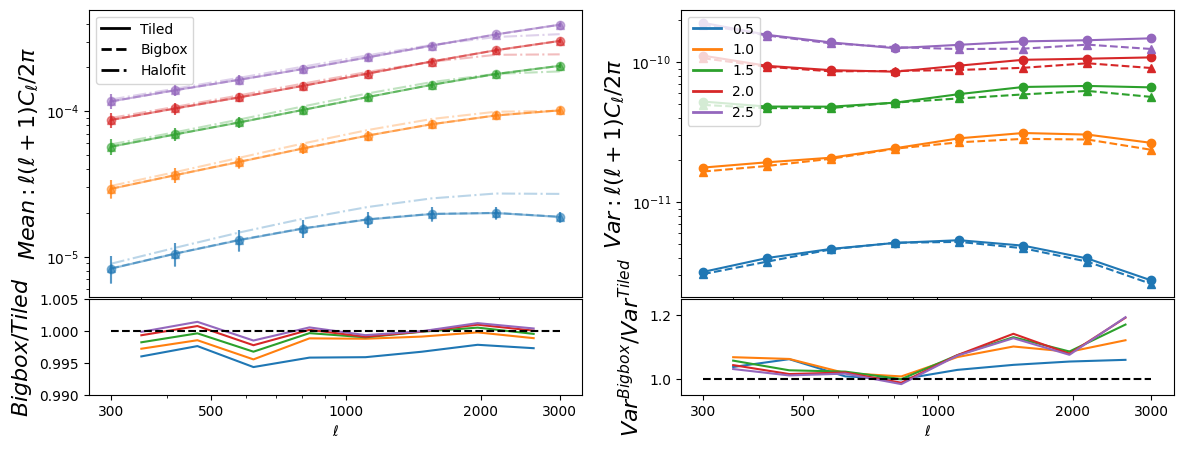
\includegraphics[width=\textwidth]{figures/results/cl_main.png}
    \caption{Comparison of the mean values of the angular power spectrum ($C^{\kappa\kappa}_{\ell}$) for different source redshifts ($z_s = 0.5, 1.0, 1.5, 2.0, 2.5$) obtained from the BIGBOX (solid lines) and TILED (dashed lines) simulations. The lower subplots show the ratio of the TILED to BIGBOX mean values, with a reference line at unity to facilitate the assessment of agreement between the two simulations.}
    \label{fig:cl_main}
    \vspace{2cm}
    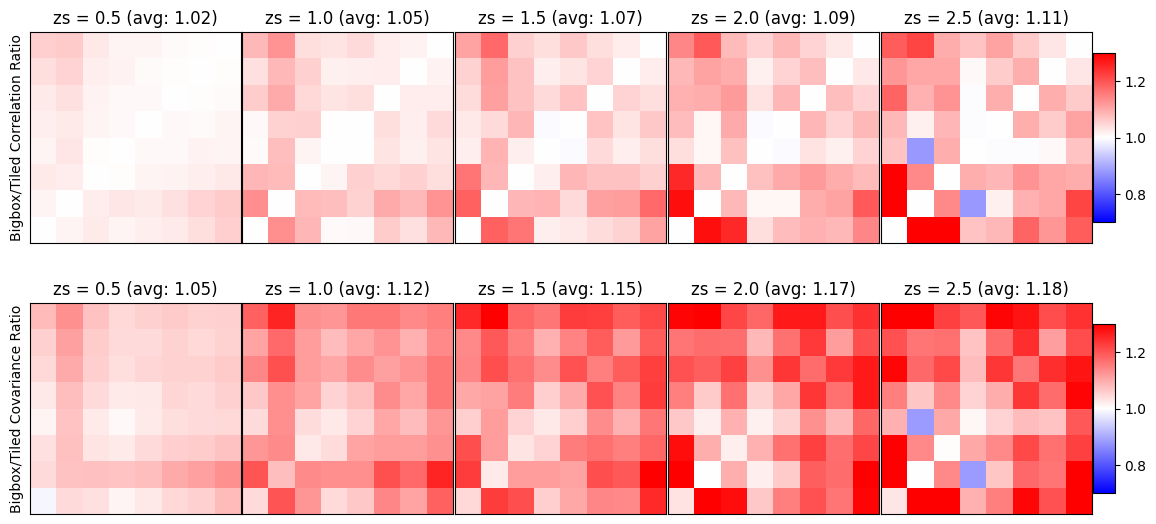
\includegraphics[width=\textwidth]{figures/results/cl_cov.png}
    \caption{Comparison of the covariance matrices and correlation matrices of the angular power spectrum ($C^{\kappa\kappa}_{\ell}$) between the BIGBOX and TILED simulations for various source redshifts ($z_s = 0.5, 1.0, 1.5, 2.0, 2.5$). The displayed ratios represent the element-wise division of the covariance and correlation matrices from the TILED simulations by those from the BIGBOX simulations. The "avg" denotes the average ratio of the considered matrix elements.}
    \label{fig:cl_cov}
\end{figure}

\begin{figure}[p]
    \centering
    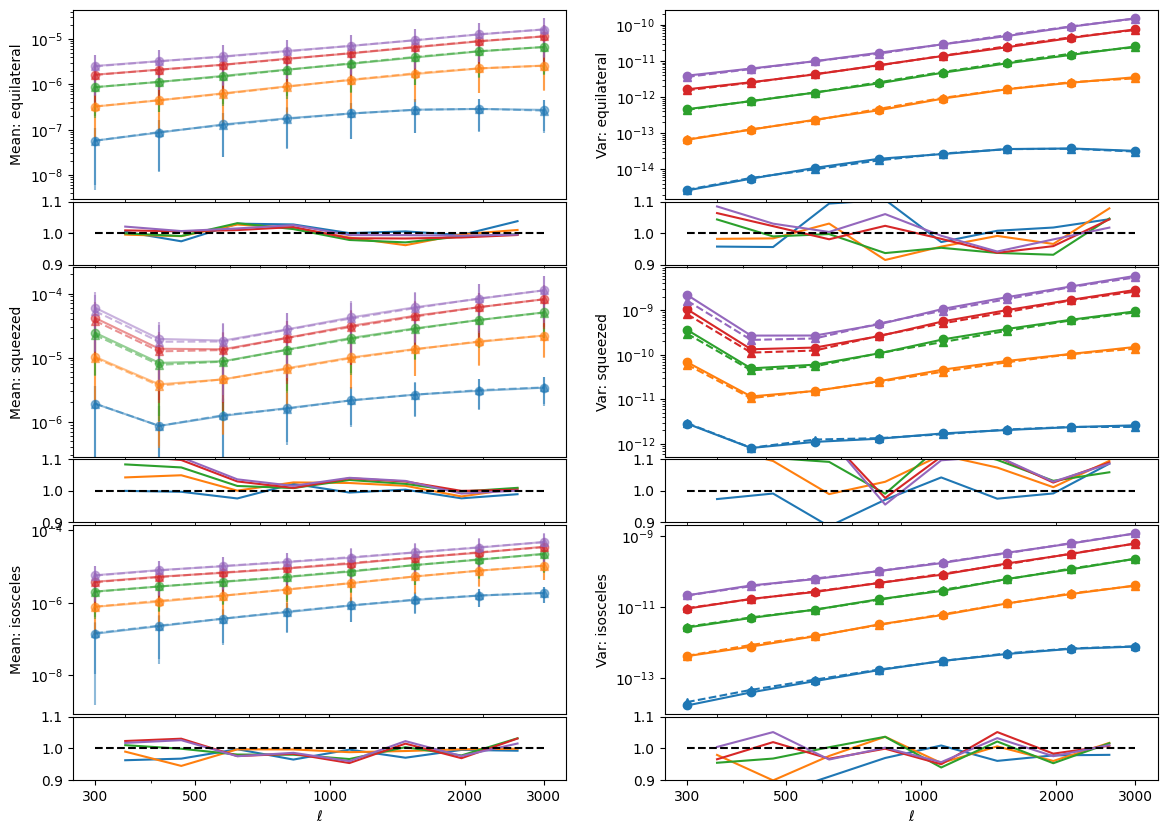
\includegraphics[width=\textwidth]{figures/results/bl_main.png}
    \caption{Same as Figure~\ref{fig:cl_main}, but for the bispectrum. }
    \label{fig:bl_main}
    \vspace{0.5cm}
    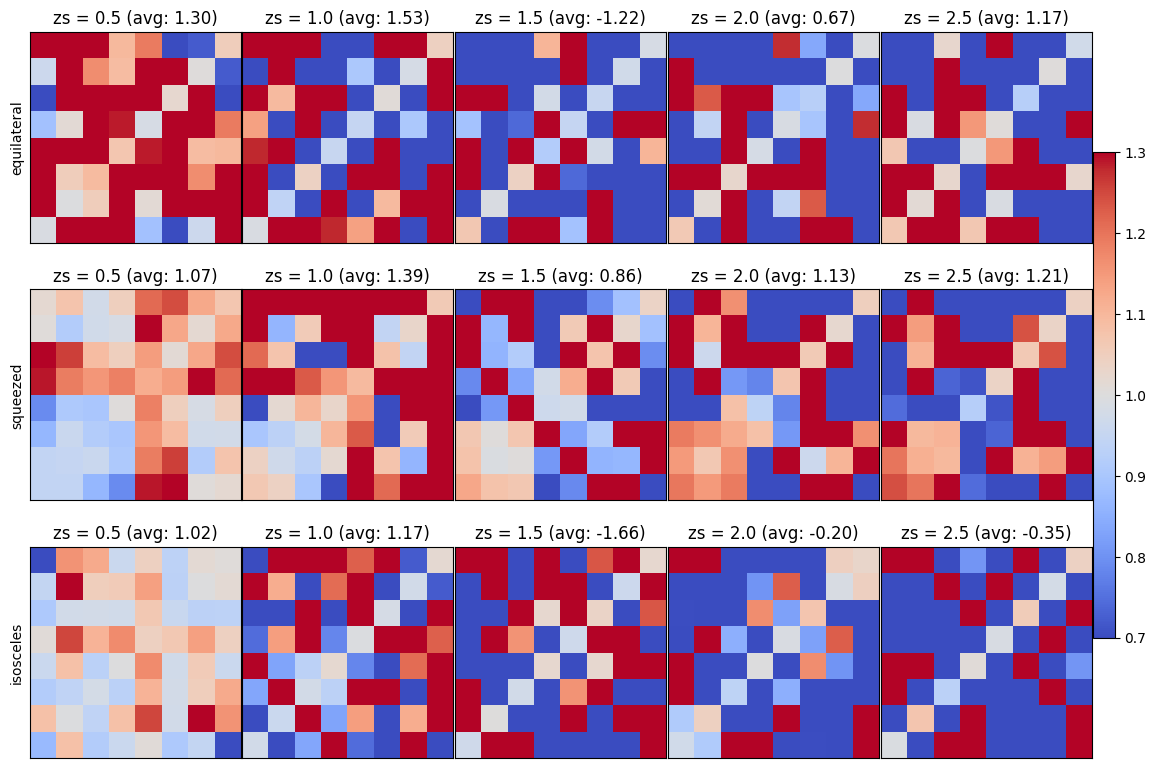
\includegraphics[width=\textwidth]{figures/results/bl_cov.png}
    \caption{Similar to Figure~\ref{fig:cl_cov}, but for the covariance matrices of the bispectrum. The noisy nature of the bispectrum covariance makes it challenging to discern clear trends between the simulations.}
    \label{fig:bl_cov}
\end{figure}

\begin{figure}[p]
    \centering
    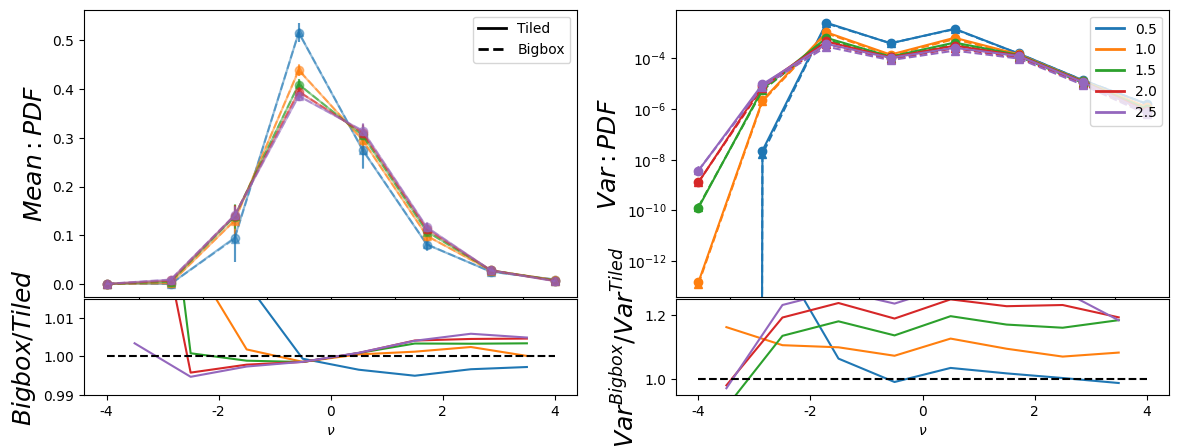
\includegraphics[width=\textwidth]{figures/results/pdf_main.png}
    \caption{Same as Figure~\ref{fig:cl_main}, but for the probability density function (PDF) of the convergence field. The comparison highlights the agreement in mean PDF values between the simulations across different redshifts.}
    \label{fig:pdf_main}
    \vspace{2cm}
    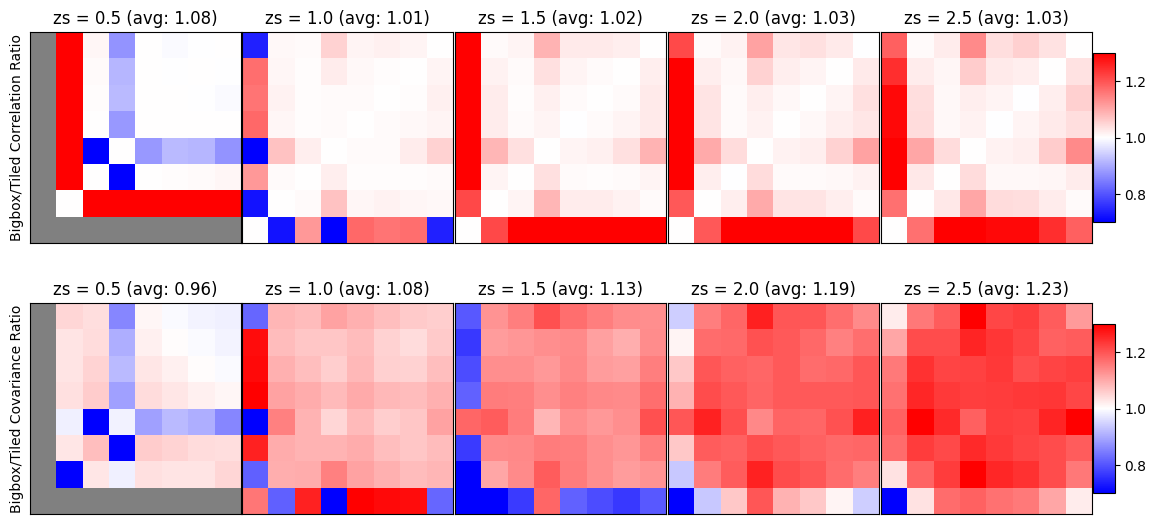
\includegraphics[width=\textwidth]{figures/results/pdf_cov.png}
    \caption{Same as Figure~\ref{fig:cl_cov}, but for the covariance matrices of the PDF. The covariance ratios indicate higher covariance in the BIGBOX simulations, particularly at higher redshifts.}
    \label{fig:pdf_cov}
\end{figure}

\begin{figure}[p]
    \centering
    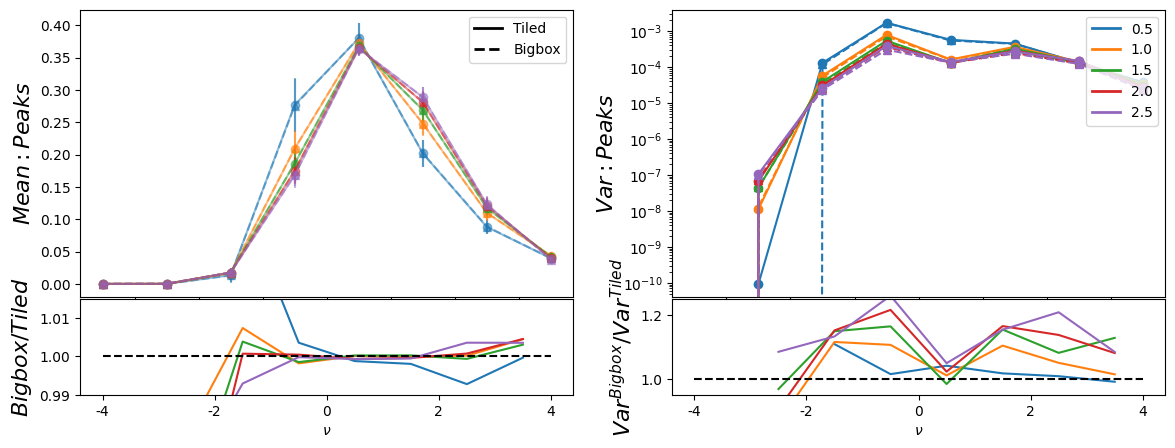
\includegraphics[width=\textwidth]{figures/results/peaks_main.png}
    \caption{Same as Figure~\ref{fig:cl_main}, but for peak counts in the convergence maps. The analysis reveals deviations at low $\nu$ values due to resolution limitations affecting low-density regions.}
    \label{fig:peak_main}
    \vspace{2cm}
    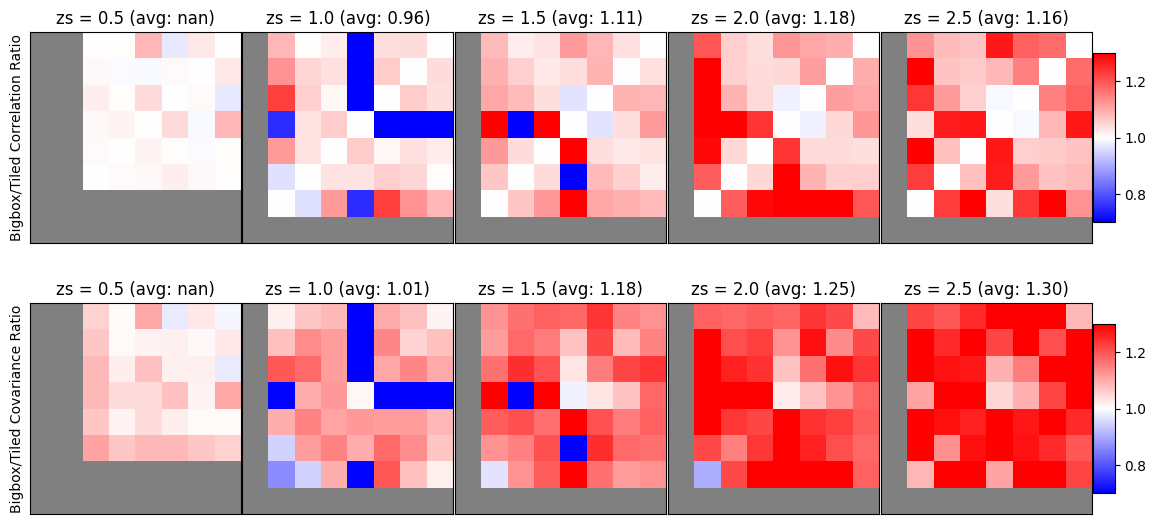
\includegraphics[width=\textwidth]{figures/results/peaks_cov.png}
    \caption{Same as Figure~\ref{fig:cl_cov}, but for the covariance matrices of peak counts. The covariance ratios suggest increased covariance in the BIGBOX simulations, with pronounced effects at higher redshifts.}
    \label{fig:peak_cov}
\end{figure}

\begin{figure}[p]
    \centering
    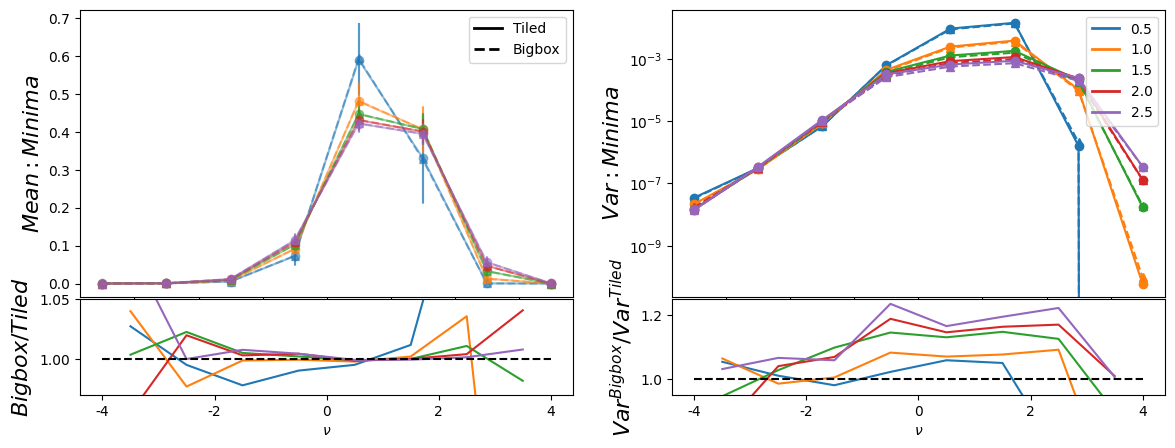
\includegraphics[width=\textwidth]{figures/results/minima_main.png}
    \caption{Same as Figure~\ref{fig:cl_main}, but for minima in the convergence maps. The comparison underscores the simulation's limitations at resolving low-density minima accurately.}
    \label{fig:min_main}
    \vspace{2cm}
    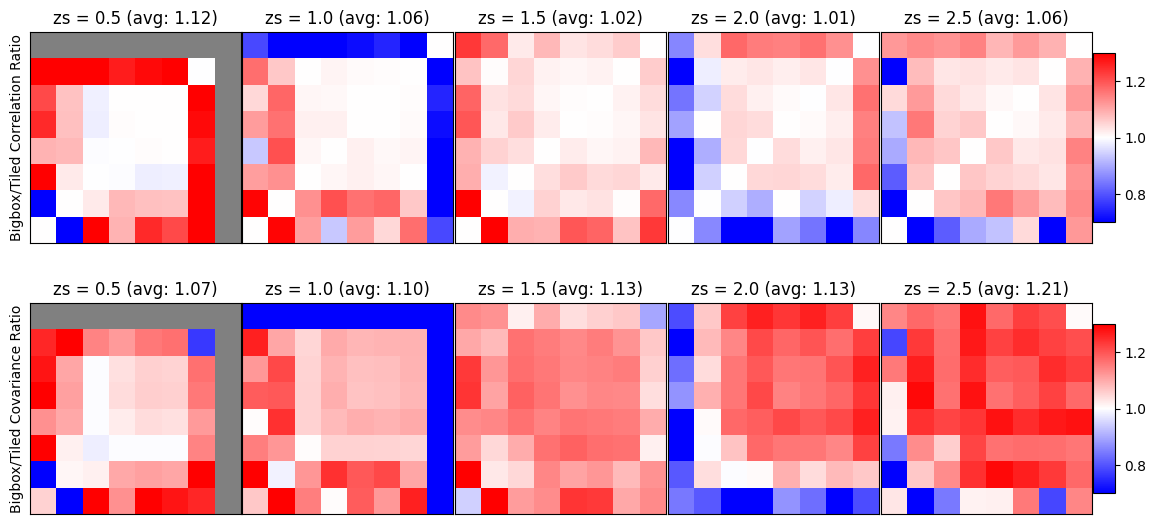
\includegraphics[width=\textwidth]{figures/results/minima_cov.png}
    \caption{Same as Figure~\ref{fig:cl_cov}, but for the covariance matrices of minima. The covariance ratios reflect higher values in the BIGBOX simulations, consistent with other statistical measures.}
    \label{fig:min_cov}
\end{figure}

\begin{figure}[p]
    \centering
    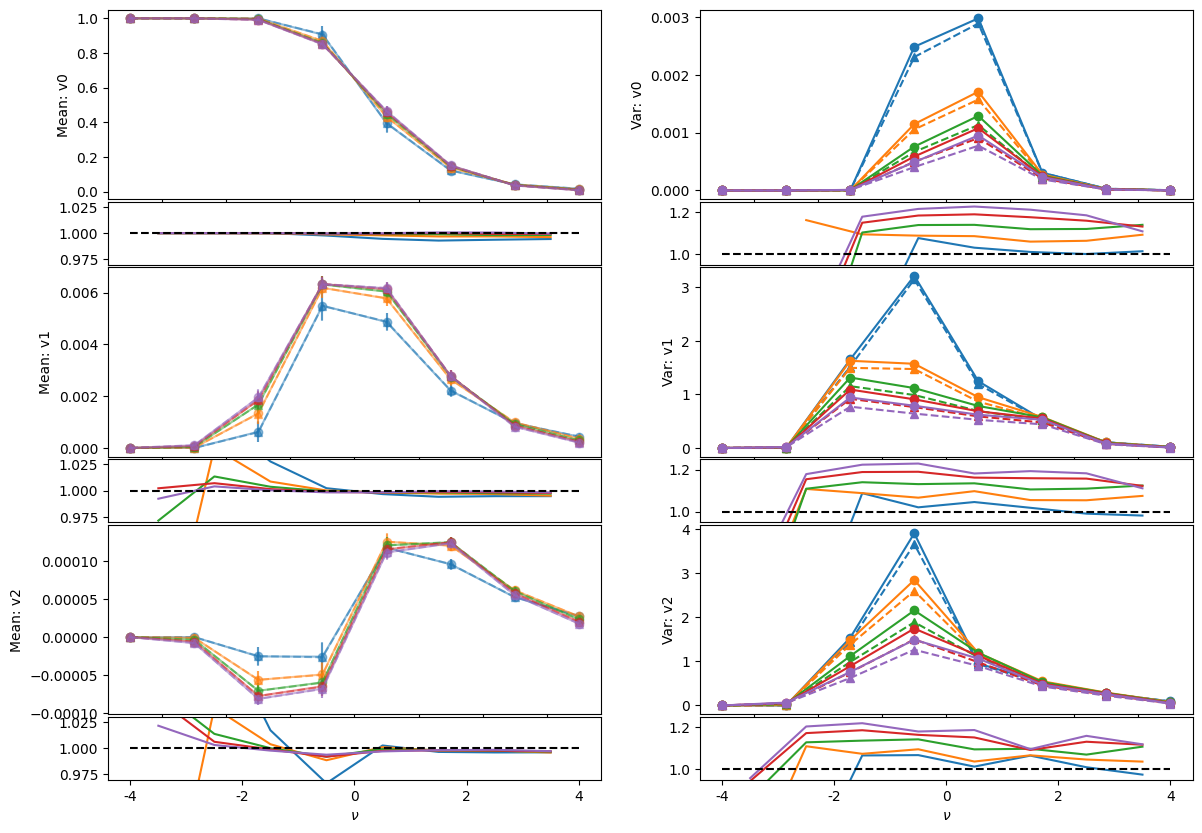
\includegraphics[width=\textwidth]{figures/results/mfs_main.png}
    \caption{Same as Figure~\ref{fig:cl_main}, but for Minkowski Functionals (area $V_0$, perimeter $V_1$, and genus $V_2$). The agreement in mean values between simulations is generally good, with some discrepancies at extreme density thresholds.}
    \label{fig:mfs_main}
    \vspace{0.5cm}
    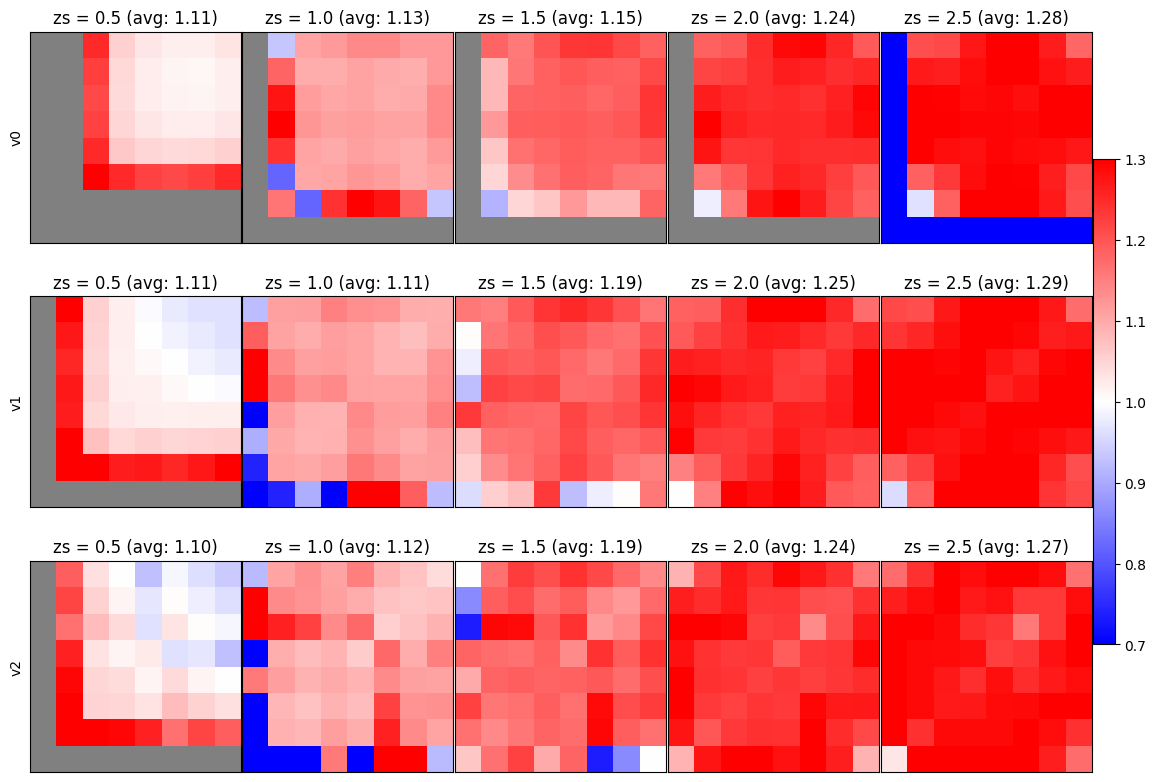
\includegraphics[width=\textwidth]{figures/results/mfs_cov.png}
    \caption{Similar to Figure~\ref{fig:cl_cov}, but for the covariance matrices of Minkowski Functionals. }
    \label{fig:mfs_cov}
\end{figure}

\section{Effects of Noise}
To assess the impact of observational noise, we have introduced five different shape noise levels into the simulations. Due to the significant influence of noise on higher-order statistics, the bispectrum has been excluded from this part of the analysis.

Figures~\ref{fig:avg_noise_cov} and \ref{fig:avg_noise_corr} illustrate how the average ratios of covariance matrices and correlation matrices change with varying shape noise levels. Except for the angular power spectrum, the non-Correlation statistics exhibit stable covariance ratios across different noise levels. 

\begin{figure}
    \centering
    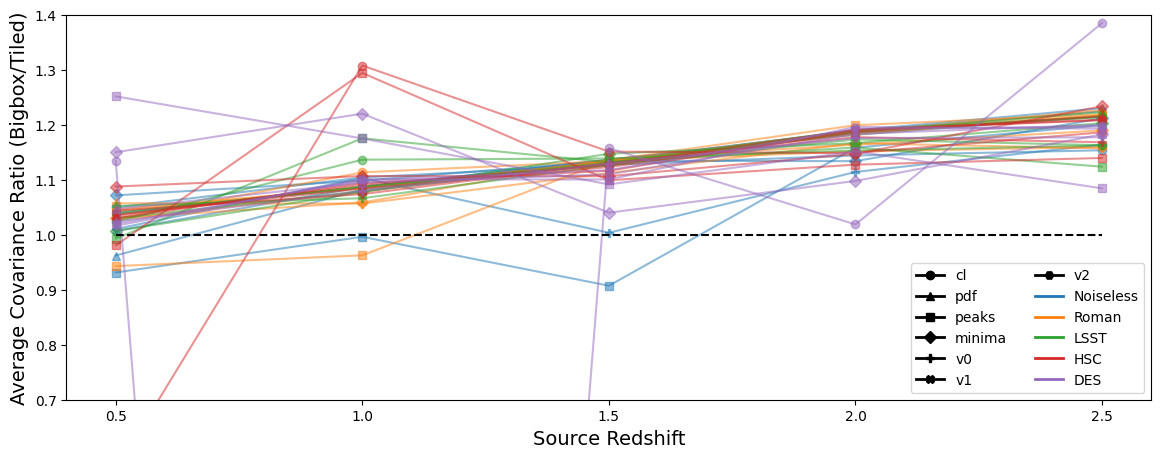
\includegraphics[width=0.6\textwidth]{figures/results/avg_cov_ratio_ngal.png}
    \caption{Average ratio of covariance matrices of statistical measures between the BIGBOX and TILED simulations for different shape noise levels (see Table~\ref{tab:noise}). The increasing trend indicates does not affected by the noise level.}
    \label{fig:avg_noise_cov}
    \vspace{0.5cm}
    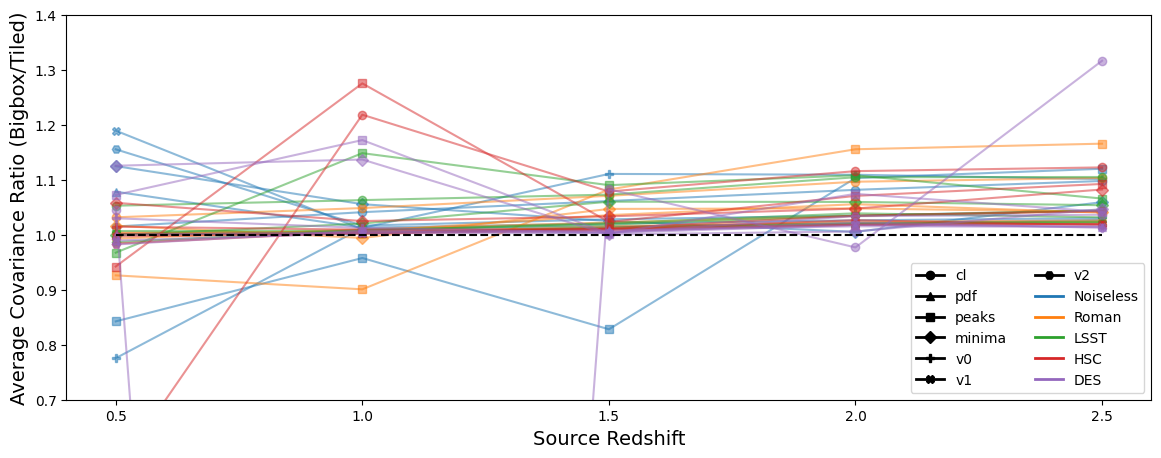
\includegraphics[width=0.6\textwidth]{figures/results/avg_corr_ratio_ngal.png}
    \caption{Same as Figure~\ref{fig:avg_noise_cov}, but for the correlation matrices. The off-diagonal elements compared to the diagonal elements do not show a clear trend with noise levels.}
    \label{fig:avg_noise_corr}
    \vspace{0.5cm}
    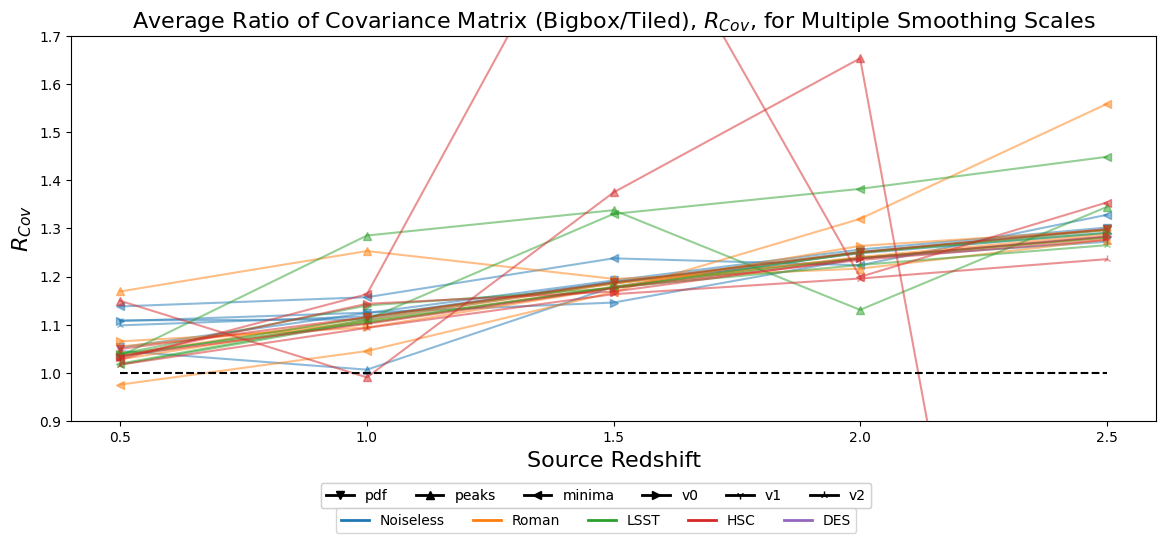
\includegraphics[width=0.6\textwidth]{figures/results/avg_cov_ratio_sl.png}
    \caption{Average ratio of covariance matrices of statistical measures between the BIGBOX and TILED simulations for different smoothing scales. Larger smoothing scales lead to increased discrepancies in covariance estimates due to the loss of small-scale information.}
    \label{fig:avg_sl_cov}
    \vspace{0.5cm}
    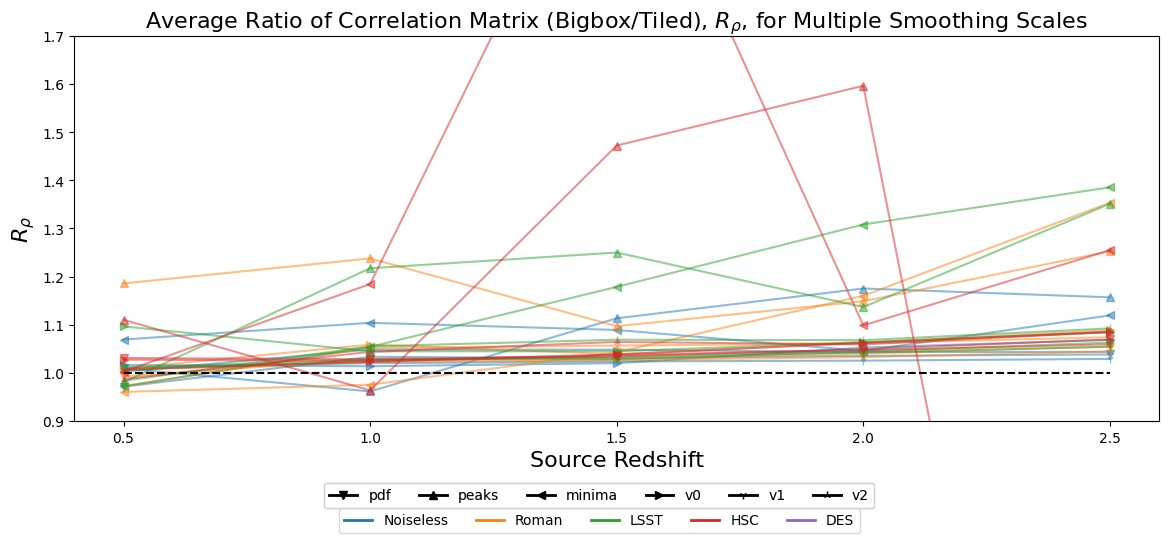
\includegraphics[width=0.6\textwidth]{figures/results/avg_corr_ratio_sl.png}
    \caption{Same as Figure~\ref{fig:avg_sl_cov}, but for the correlation matrices. The instability at larger smoothing scales reflects the challenges in capturing correlations at reduced resolutions.}
    \label{fig:avg_sl_corr}
\end{figure}

Figures~\ref{fig:cl_noise} and \ref{fig:ng_noise} demonstrate how the ratios of covariance matrices for the angular power spectrum and the non-correlation statistics change with different shape noise levels. The results indicate that the angular power spectrum and minima are particularly sensitive to the shape noise level, exhibiting significant variations in their covariance matrices. In contrast, other non-correlation statistics remain more robust against changes in the shape noise level, maintaining relatively stable off-diagonal elements in their covariance matrices.

\begin{figure}[p]
    \centering
    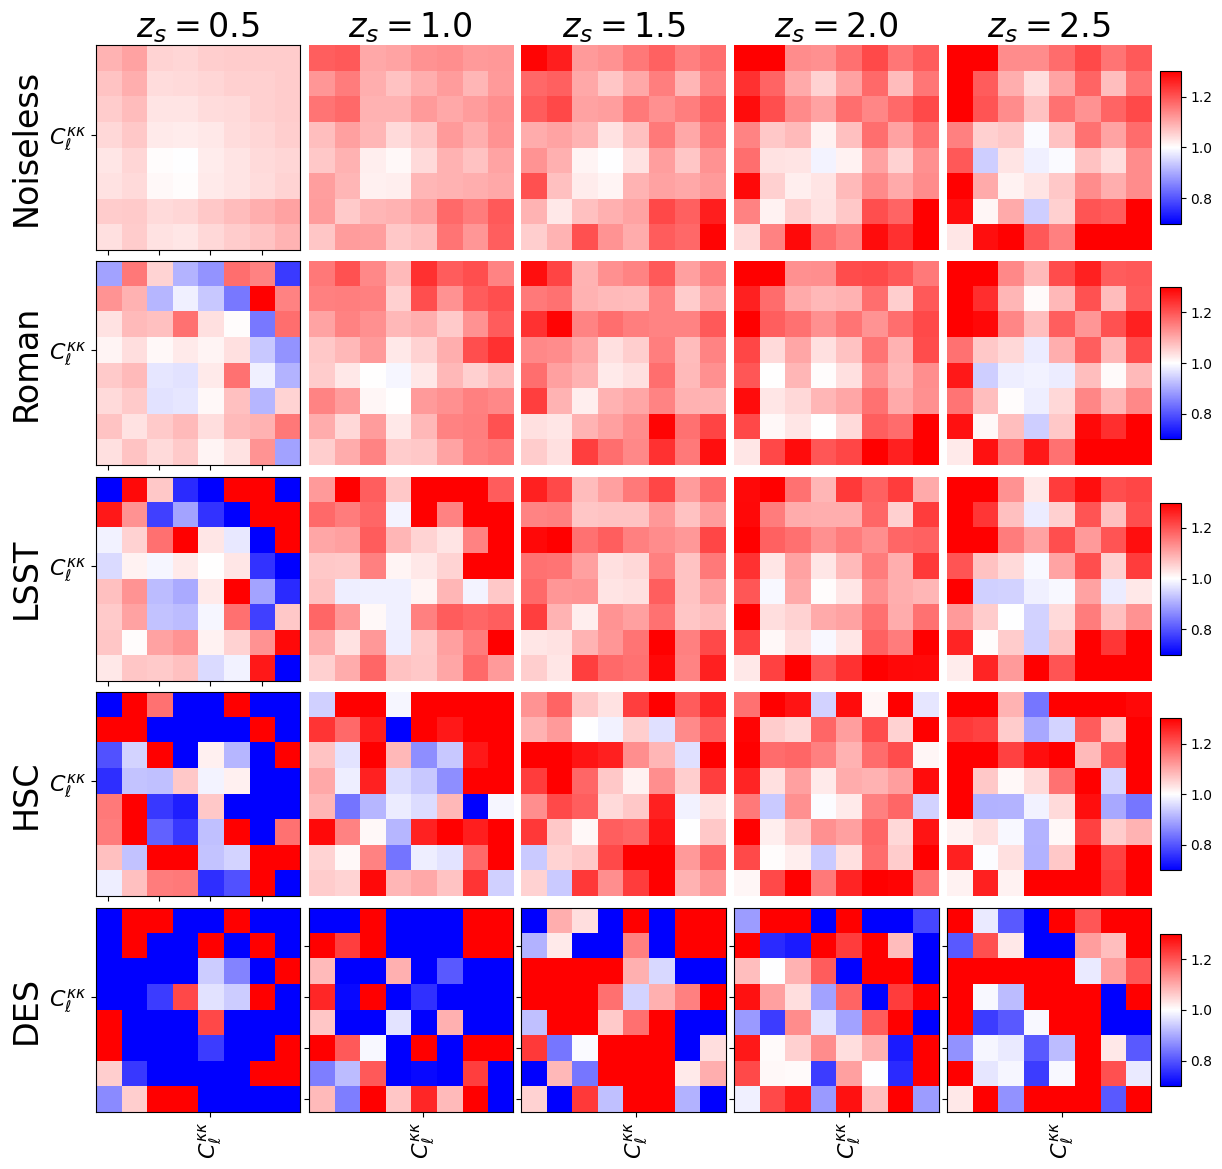
\includegraphics[width=0.6\textwidth]{figures/results/correlation_cov_noise.png}
    \caption{Ratio of covariance matrices of the angular power spectrum ($C^{\kappa\kappa}_{\ell}$) between the BIGBOX and TILED simulations for different shape noise levels (see Table~\ref{tab:noise}). The sensitivity of the power spectrum to noise is evident from the fluctuating covariance ratios with higher noise levels.}
    \label{fig:cl_noise}
    \vspace{0.5cm}
    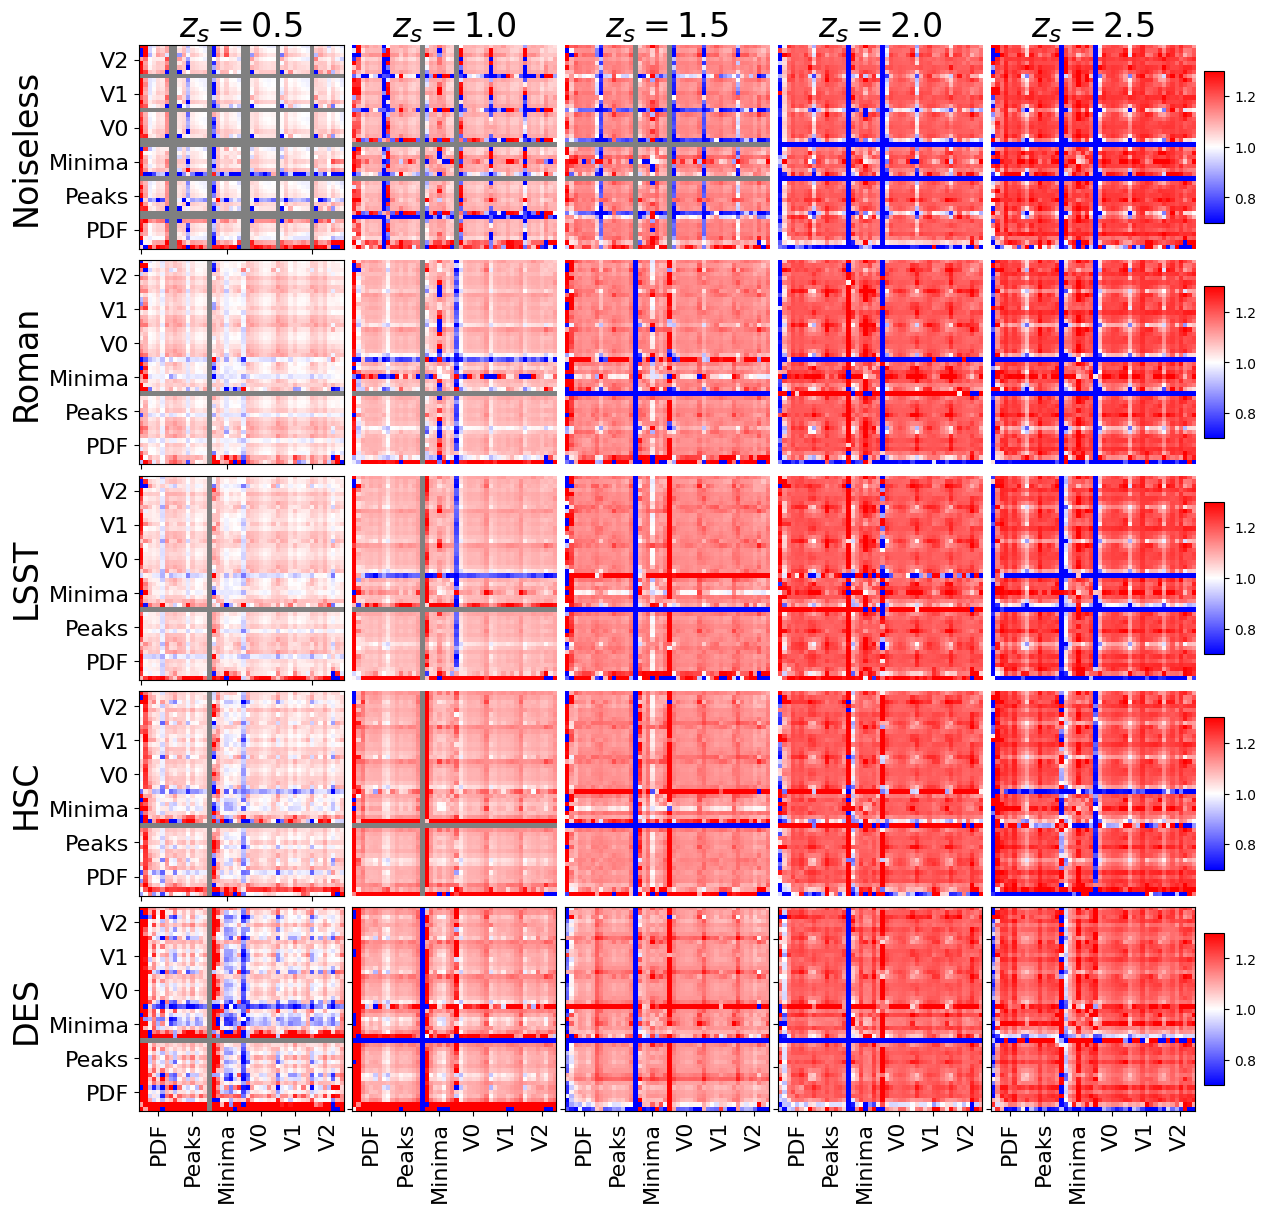
\includegraphics[width=0.8\textwidth]{figures/results/nongaussian_cov_noise.png}
    \caption{Same as Figure~\ref{fig:cl_noise}, but for the non-Gaussian statistical measures. The robustness of these measures against noise variations is reflected in the relatively stable covariance ratios.}
    \label{fig:ng_noise}
\end{figure}

\section{Effects of Smoothing Scale}
To evaluate the impact of smoothing on the statistical measures, we have applied four different smoothing scales to the simulations. Smoothing affects the resolution of the convergence maps and can influence the detection of small-scale structures.

Figures~\ref{fig:avg_sl_cov} and \ref{fig:avg_sl_corr} show how the average ratios of covariance matrices and correlation matrices change with varying smoothing scales. The ratios become more unstable due to the smoothing effect washing out small-scale structures.

Figure~\ref{fig:ng_smoothing} illustrates the effects of smoothing scale on non-Correlation statistical measures. As the smoothing scale increases, the finer structures in the convergence maps are blurred, leading to changes in the statistical properties. The blank bins that previously contained little or no signal begin to be filled due to the spread of signals from neighboring bins, while the overall signal intensity is redistributed.

\begin{figure}
    \centering
    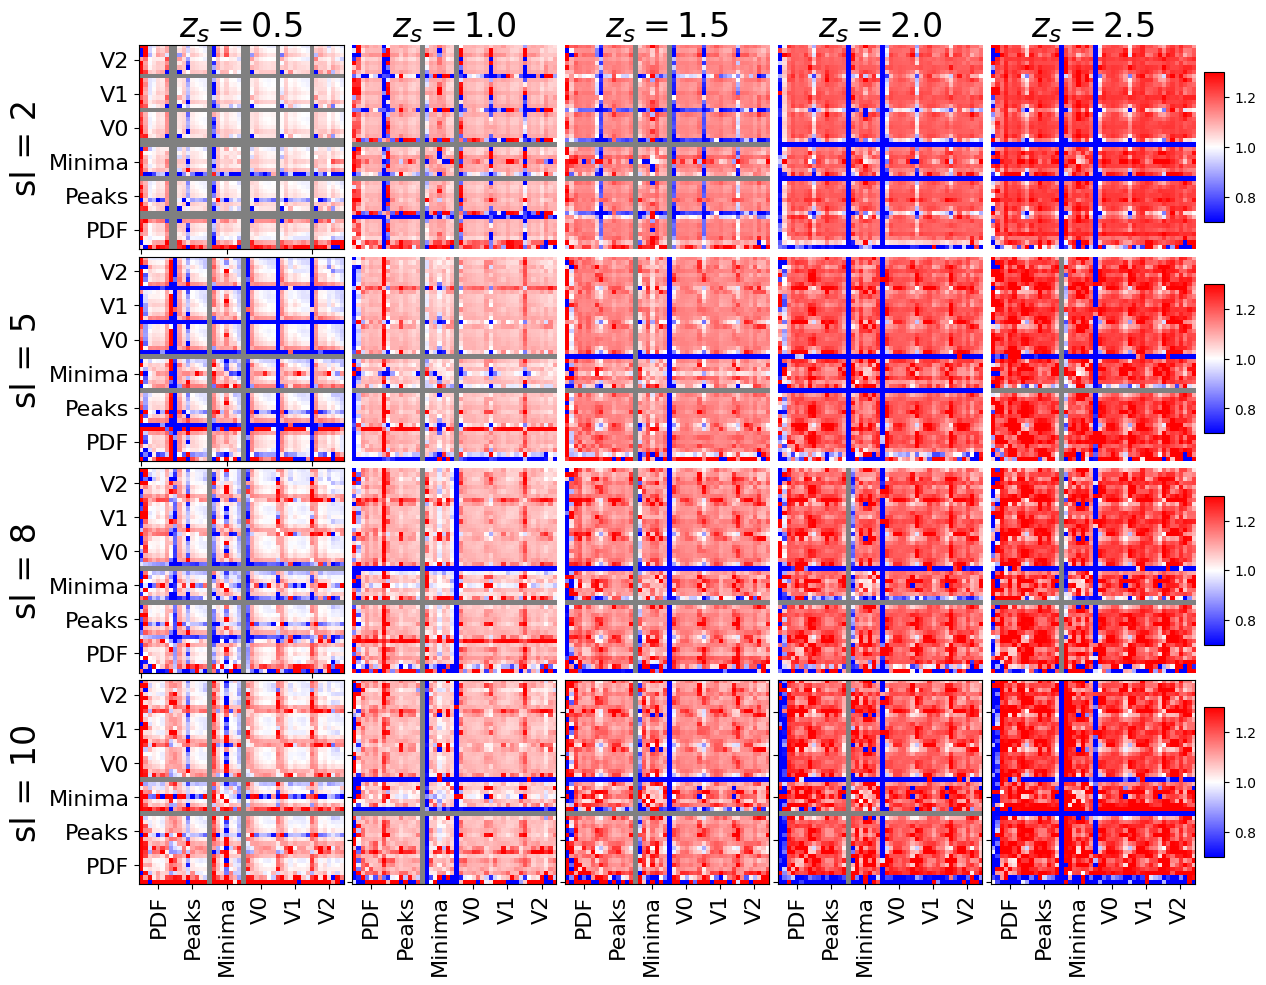
\includegraphics[width=0.8\textwidth]{figures/results/nongaussian_cov_sl.png}
    \caption{Same as Figure~\ref{fig:ng_noise}, but showing the impact of different smoothing scales on the covariance matrices of non-Gaussian statistical measures. The results emphasize how increased smoothing affects the detection and characterization of small-scale features.}
    \label{fig:ng_smoothing}
\end{figure}

\chapter{Discussion}
\section{Source of Systematics}
In this section, we will discuss the possible sources of systematics that could affect the covariance matrix. 

\subsection{Box Replication Effect}
The box replication effect arises from the re



\section{Possible Effects}
In this section, we will consider possible effects that could affect the covariance matrix, except for the super-sample covariance.
\subsection{Finite Support Effects}
Finite support effects are the effects that arise from the fact that the survey volume is finite. The finite support effects can be divided into two categories: the effects of the survey window function and the effects of the survey boundary. The survey window function is the function that describes the survey geometry, and the survey boundary is the boundary of the survey volume. The finite support effects can be understood as the effects of the survey window function and the survey boundary on the covariance matrix.

\subsection{Box Replication Effect}
It is clear that the patches lying on the equator are more tiled compared to the rest. For a rough estimation, we check the statistics of the patches lying on the equator and compare them with the rest of the patches.

\section{Validation}
We conducted simulations to validate the effects of finite support and box replication. The simulations were performed with box sizes $(L_{\text{box}}\, [\mathrm{Mpc}/h])$ of 125, 250, 500, 1000, 2000, and 4000, corresponding to particle numbers $(N_{\text{part}})$ of $125^3$, $250^3$, $500^3$, $1000^3$, $2000^3$, and $4000^3$, respectively. The simulations cover redshifts from $0$ to $3$, and for each set of parameters, we generated 5 realizations.

We check the statistics for each simulation boxes and compare them each other.



\section{Check if the gnomview matters}

\section{Why higher-order statistics are less affected?}

\section{correlation between different smoothing scales}






% \chapter{Conclusions and Future Work}
% \section{Summary of Key Findings}
% This thesis demonstrated the importance of accounting for artefacts in weak lensing simulations to improve covariance matrix estimations.

% \section{Limitations and Future Work}
% Future research could explore more complex simulations and apply findings to LSST and Roman surveys.

% \appendix  % Start of appendices

% \chapter{Additional Mathematical Derivations}
% Here you can include detailed derivations that were omitted from the main text.

\bibliographystyle{mnras}
\bibliography{thesis_bib.bib}

\end{document}